\section{Espacios Vectoriales Euclídeos.}
\label{sec:EjerciciosTema3}
\begin{ejercicio} \label{Ejercicio1}
Encontrar la matriz respecto de la base usual de la proyección $p$ y de la reflexión $s$ respecto de los siguientes subespacios:
\begin{enumerate}
    \item En el EVME $(\bb{R}^2,\langle,\rangle)$
    \begin{equation*}
        L_1=\cc{L}\left\{\left(\begin{array}{c}
             1 \\ 2
        \end{array}\right)\right\}
        \qquad
        L_2=\cc{L}\left\{\left(\begin{array}{c}
             -3 \\ 4
        \end{array}\right)\right\}
        \qquad
        L_3 \equiv x+3y=0
        \qquad
        L_4=(L_1)^\perp
    \end{equation*}

    \begin{enumerate}
        \item $L_1=\cc{L}\left\{\left(\begin{array}{c}
             1 \\ 2
        \end{array}\right)\right\}$

        Tengo que $(L_1)^\perp=\cc{L}\left\{\left(\begin{array}{c}
             2 \\ -1
        \end{array}\right)\right\}$.

        Por tanto, $\cc{B}=\left\{\left(\begin{array}{c}
             1 \\ 2
        \end{array}\right), \left(\begin{array}{c}
             2 \\ -1
        \end{array}\right)\right\}$ es una base de vectores ortogonales, y 
        $\bar{\cc{B}}=\left\{\frac{1}{\sqrt{5}}\left(\begin{array}{c}
             1 \\ 2
        \end{array}\right), \frac{1}{\sqrt{5}}\left(\begin{array}{c}
             2 \\ -1
        \end{array}\right)\right\}$ es una base ortonormal.

        %Consideramos la base usual $\cc{B}_u=\{e_1, e_2\}$.
        Sea $v=(x_1,x_2)_{\cc{B}_u}=(a_1,a_2)_{\bar{\cc{B}}}\in \bb{R}^2$. Como $\cc{B}$ es una base ortonormal, tenemos que:
        \begin{equation*}
            a_1=\left\langle \frac{1}{\sqrt{5}}\left(\begin{array}{c}
             1 \\ 2
        \end{array}\right), v\right\rangle = \frac{1}{\sqrt{5}}(x_1+2x_2)
        \end{equation*}

        Por la elección de la base ortonormal, tenemos que:
        \begin{multline*}
            p_{L_1}(v)=a_1\cdot \frac{1}{\sqrt{5}}\left(\begin{array}{c}
                 1 \\ 2
            \end{array}\right)
            =\frac{1}{\sqrt{5}}(x_1+2x_2) \cdot \frac{1}{\sqrt{5}}\left(\begin{array}{c}
                 1 \\ 2
            \end{array}\right)
            =\frac{1}{5} \left(\begin{array}{c}
                 x_1+2x_2 \\ 2x_1+4x_2
            \end{array}\right)
            =\\=
            \frac{1}{5}\left(\begin{array}{cc}
                1 & 2 \\
                2 & 4
            \end{array}\right)\left(\begin{array}{c}
                 x_1 \\ x_2
            \end{array}\right)
        \end{multline*}

        Por tanto, tenemos que:
        \begin{equation*}
            M(p_{L_1},\cc{B}_u) = \frac{1}{5}\left(\begin{array}{cc}
                1 & 2 \\
                2 & 4
            \end{array}\right)
        \end{equation*}

        Además, como tenemos que:
        \begin{gather*}
            p_L +P_{L^\perp} = Id \Longrightarrow p_{L^\perp} = Id -p_L\\
            s_L = p_L - P_{L^\perp} = 2p_L -Id
        \end{gather*}

        Por tanto,
        \begin{equation*}
            M(s_{L_1},\cc{B}_u) = \frac{2}{5}\left(\begin{array}{cc}
                1 & 2 \\
                2 & 4
            \end{array}\right) - \left(\begin{array}{cc}
                1 & 0 \\
                0 & 1
            \end{array}\right)
            = \frac{1}{5}\left(\begin{array}{cc}
                -3 & 4 \\
                4 & 3
            \end{array}\right)
        \end{equation*}



        \item $L_2=\cc{L}\left\{\left(\begin{array}{c}
             -3 \\ 4
        \end{array}\right)\right\}$

        Tengo que $(L_2)^\perp=\cc{L}\left\{\left(\begin{array}{c}
             4 \\ 3
        \end{array}\right)\right\}$.

        Por tanto, $\cc{B}=\left\{\left(\begin{array}{c}
             -3 \\ 4
        \end{array}\right), \left(\begin{array}{c}
             4 \\ 3
        \end{array}\right)\right\}$ es una base de vectores ortogonales, y 
        $\bar{\cc{B}}=\left\{\frac{1}{5}\left(\begin{array}{c}
            -3 \\ 4
        \end{array}\right), \frac{1}{5}\left(\begin{array}{c}
             4 \\ 3
        \end{array}\right)\right\}$ es una base ortonormal.

        Sea $v=(x_1,x_2)_{\cc{B}_u}=(a_1,a_2)_{\bar{\cc{B}}}\in \bb{R}^2$. Como $\cc{B}$ es una base ortonormal, tenemos que:
        \begin{equation*}
            a_1=\left\langle \frac{1}{5}\left(\begin{array}{c}
             -3 \\ 4
        \end{array}\right), v\right\rangle = \frac{1}{5}(-3x_1+4x_2)
        \end{equation*}

        Por la elección de la base ortonormal, tenemos que:
        \begin{multline*}
            p_{L_2}(v)=a_1\cdot \frac{1}{5}\left(\begin{array}{c}
                 -3 \\ 4
            \end{array}\right)
            =\frac{1}{5}(-3x_1+4x_2) \cdot \frac{1}{5}\left(\begin{array}{c}
                 -3 \\ 4
            \end{array}\right)
            =\frac{1}{5^2} \left(\begin{array}{c}
                 9x_1-12x_2 \\ -12x_1+16x_2
            \end{array}\right)
            =\\=
            \frac{1}{5^2}\left(\begin{array}{cc}
                9 & -12 \\
                -12 & 16
            \end{array}\right)\left(\begin{array}{c}
                 x_1 \\ x_2
            \end{array}\right)
        \end{multline*}

        Por tanto, tenemos que:
        \begin{equation*}
            M(p_{L_2},\cc{B}_u) = \frac{1}{25}\left(\begin{array}{cc}
                9 & -12 \\
                -12 & 16
            \end{array}\right)
        \end{equation*}

        Además, como tenemos que:
        \begin{gather*}
            p_L +P_{L^\perp} = Id \Longrightarrow p_{L^\perp} = Id -p_L\\
            s_L = p_L - P_{L^\perp} = 2p_L -Id
        \end{gather*}

        Por tanto,
        \begin{equation*}
            M(s_{L_2},\cc{B}_u) =\frac{2}{25}\left(\begin{array}{cc}
                9 & -12 \\
                -12 & 16
            \end{array}\right) - \left(\begin{array}{cc}
                1 & 0 \\
                0 & 1
            \end{array}\right)
            = \frac{1}{25}\left(\begin{array}{cc}
                -7 & -24 \\
                -24 & 7
            \end{array}\right)
        \end{equation*}



        \item $L_3\equiv x+3y=0\equiv \cc{L}\left\{\left(\begin{array}{c}
             -3 \\ 1
        \end{array}\right)\right\}$

        Tengo que $(L_3)^\perp=\cc{L}\left\{\left(\begin{array}{c}
             1 \\ 3
        \end{array}\right)\right\}$.

        Por tanto, $\cc{B}=\left\{\left(\begin{array}{c}
             -3 \\ 1
        \end{array}\right), \left(\begin{array}{c}
             1 \\ 3
        \end{array}\right)\right\}$ es una base de vectores ortogonales, y 
        $\bar{\cc{B}}=\left\{\frac{1}{\sqrt{10}}\left(\begin{array}{c}
            -3 \\ 1
        \end{array}\right), \frac{1}{\sqrt{10}}\left(\begin{array}{c}
             1 \\ 3
        \end{array}\right)\right\}$ es una base ortonormal.

        Sea $v=(x_1,x_2)_{\cc{B}_u}=(a_1,a_2)_{\bar{\cc{B}}}\in \bb{R}^2$. Como $\cc{B}$ es una base ortonormal, tenemos que:
        \begin{equation*}
            a_1=\left\langle \frac{1}{\sqrt{10}}\left(\begin{array}{c}
             -3 \\ 1
        \end{array}\right), v\right\rangle = \frac{1}{\sqrt{10}}(-3x_1+x_2)
        \end{equation*}

        Por la elección de la base ortonormal, tenemos que:
        \begin{multline*}
            p_{L_3}(v)=a_1\cdot \frac{1}{\sqrt{10}}\left(\begin{array}{c}
                 -3 \\ 1
            \end{array}\right)
            =\frac{1}{\sqrt{10}}(-3x_1+x_2) \cdot \frac{1}{\sqrt{10}}\left(\begin{array}{c}
                 -3 \\ 1
            \end{array}\right)
            =\frac{1}{10} \left(\begin{array}{c}
                 9x_1-3x_2 \\ -3x_1+x_2
            \end{array}\right)
            =\\=
            \frac{1}{10}\left(\begin{array}{cc}
                9 & -3 \\
                -3 & 1
            \end{array}\right)\left(\begin{array}{c}
                 x_1 \\ x_2
            \end{array}\right)
        \end{multline*}

        Por tanto, tenemos que:
        \begin{equation*}
            M(p_{L_3},\cc{B}_u) = \frac{1}{10}\left(\begin{array}{cc}
                9 & -3 \\
                -3 & 1
            \end{array}\right)
        \end{equation*}

        Además, como tenemos que:
        \begin{gather*}
            p_L +P_{L^\perp} = Id \Longrightarrow p_{L^\perp} = Id -p_L\\
            s_L = p_L - P_{L^\perp} = 2p_L -Id
        \end{gather*}

        Por tanto,
        \begin{equation*}
            M(s_{L_3},\cc{B}_u) =\frac{2}{10}\left(\begin{array}{cc}
                9 & -3 \\
                -3 & 1
            \end{array}\right) - \left(\begin{array}{cc}
                1 & 0 \\
                0 & 1
            \end{array}\right)
            = \frac{1}{5}\left(\begin{array}{cc}
                4 & -3 \\
                -3 & -4
            \end{array}\right)
        \end{equation*}


        \item $L_4=(L_1)^\perp$

        Como se ha visto, tenemos que:
        \begin{equation*}
            M(p_{L_1},\cc{B}_u) = \frac{1}{5}\left(\begin{array}{cc}
                1 & 2 \\
                2 & 4
            \end{array}\right)
        \end{equation*}

        Como $p_L +P_{L^\perp} = Id \Longrightarrow p_{L^\perp} = Id -p_L$, entonces:
        \begin{equation*}
            M(p_{L_4},\cc{B}_u) = \frac{1}{5}\left(\begin{array}{cc}
                4 & -2 \\
                -2 & 1
            \end{array}\right)
        \end{equation*}

        Además, como tenemos que:
        \begin{gather*}
            p_L +P_{L^\perp} = Id \Longrightarrow p_{L^\perp} = Id -p_L\\
            s_L = p_L - P_{L^\perp} = 2p_L -Id
        \end{gather*}

        Por tanto,
        \begin{equation*}
            M(s_{L_4},\cc{B}_u) = \frac{2}{5}\left(\begin{array}{cc}
                4 & -2 \\
                -2 & 1
            \end{array}\right) - \left(\begin{array}{cc}
                1 & 0 \\
                0 & 1
            \end{array}\right)
            = \frac{1}{5}\left(\begin{array}{cc}
                3 & -4 \\
                -4 & -3
            \end{array}\right)
        \end{equation*}
    \end{enumerate}

        


    \item En el EVME $(\bb{R}^3,\langle,\rangle)$ \label{Ej1.2}
    \begin{equation*}
        L_1=\cc{L}\left\{\left(\begin{array}{c}
             1 \\ 1 \\ 1
        \end{array}\right)\right\}
        \qquad
        \Pi_2\equiv -x+y=0
        \qquad
        \Pi_3 \equiv x+2y-z=0
        \qquad
        \Pi_4=(L_1)^\perp
    \end{equation*}

    \begin{enumerate}
        \item $L_1=\cc{L}\left\{\left(\begin{array}{c} \label{Ej1.2.a_Recta111}
             1 \\ 1 \\ 1
        \end{array}\right)\right\}$

        Sea $\cc{B}=\{e_1, e_2, e_3\}=\left\{
                \left(\begin{array}{c}
                     1 \\ 1 \\ 1
                \end{array}\right),e_2, e_3\right\}$
        base ortogonal de $V$, que existe por el Teorema de Sylvester.
        
        Sea $\bar{\cc{B}}=\{\bar{e_1}, \bar{e_2}, \bar{e_3}\}= \left\{
            \frac{1}{\sqrt{3}}e_1,
            \bar{e_2}, \bar{e_3}
            \right\}$ base ortonormal de $V$.
        
        Sea $v=(x_1, x_2, x_3)_{\cc{B}_u}=(a_1, a_2, a_3)_{\bar{\cc{B}}}\in V$. Como $\bar{\cc{B}}$ es una base ortonormal, tengo que $a_1 = \left<v, \bar{e_1}\right>$. Por tanto:
        \begin{equation*}
            a_1 = \left<v, \bar{e_1}\right> = (x_1, x_2, x_3) \frac{1}{\sqrt{3}} e_1
            = \frac{1}{\sqrt{3}}(x_1 + x_2 + x_3)
        \end{equation*}
        
        Además, por la elección de la base ortonormal, tenemos que:
        \begin{equation*}
            p_{L_1}(v)=a_1\bar{e_1}= \frac{1}{\sqrt{3}}(x_1 + x_2 + x_3)\bar{e_1}
            = \frac{1}{3}(x_1 + x_2 + x_3)e_1
        \end{equation*}

        Por tanto, buscando la matriz que represente $p_L$, tenemos que:
        \begin{multline*}
            p_{L_1}(v)=\frac{1}{3}(x_1 + x_2 + x_3)e_1
            =\frac{1}{3}(x_1 + x_2 + x_3)\left(\begin{array}{c}
                 1 \\ 1 \\ 1
            \end{array}\right)
            =\frac{1}{3}\left(\begin{array}{c}
                 x_1 + x_2 + x_3 \\ x_1 + x_2 + x_3 \\ x_1 + x_2 + x_3
            \end{array}\right) =\\
            =\frac{1}{3}\left(\begin{array}{ccc}
                 1 & 1 & 1 \\
                 1 & 1 & 1 \\
                 1 & 1 & 1 \\
            \end{array}\right)\left(\begin{array}{c}
                 x_1 \\ x_2 \\ x_3
            \end{array}\right)
        \end{multline*}
        
        Por tanto, tenemos que:
        \begin{equation*}
            M(p_{L_1};\cc{B}_u)=\frac{1}{3}\left(\begin{array}{ccc}
                 1 & 1 & 1 \\
                 1 & 1 & 1 \\
                 1 & 1 & 1 \\
            \end{array}\right)
        \end{equation*}

        Además, como $s_L = 2p_L - Id$, tenemos que:
        \begin{equation*}
            M(s_{L_1};\cc{B}_u)=\frac{1}{3}\left(\begin{array}{ccc}
                 -1 & 2 & 2 \\
                 2 & -1 & 2 \\
                 2 & 2 & -1 \\
            \end{array}\right)
        \end{equation*}



        \item $\Pi_2\equiv -x+y=0 \equiv \cc{L}\left\{\left(\begin{array}{c}
             0 \\ 0 \\ 1
        \end{array}\right),
        \left(\begin{array}{c}
             1 \\ 1 \\ 0
        \end{array}\right)\right\}$

        Sea $\cc{B}=\{e_1, e_2, e_3\}=\left\{
                \left(\begin{array}{c}
                     0 \\ 0 \\ 1
                \end{array}\right),
                \left(\begin{array}{c}
                     1 \\ 1 \\ 0
                \end{array}\right),
                e_3\right\}$
        base ortogonal de $V$, que existe por el Teorema de Sylvester.
        
        Sea $\bar{\cc{B}}=\{\bar{e_1}, \bar{e_2}, \bar{e_3}\}= \left\{
            e_1,
            \frac{1}{\sqrt{2}}e_2, \bar{e_3}
            \right\}$ base ortonormal de $V$.
        
        Sea $v=(x_1, x_2, x_3)_{\cc{B}_u}=(a_1, a_2, a_3)_{\bar{\cc{B}}}\in V$. Como $\bar{\cc{B}}$ es una base ortonormal, tengo que $a_i = \left<v, \bar{e_i}\right>$. Por tanto:
        \begin{equation*}
            a_1 = \left<v, \bar{e_1}\right> = (x_1, x_2, x_3) e_1
            = x_3
        \end{equation*}
        \begin{equation*}
            a_2 = \left<v, \bar{e_2}\right> = (x_1, x_2, x_3) \frac{1}{\sqrt{2}} e_2
            = \frac{1}{\sqrt{2}}(x_1 + x_2)
        \end{equation*}
        
        Además, por la elección de la base ortonormal, tenemos que:
        \begin{equation*}
            p_{\Pi_2}(v)=a_1\bar{e_1} +a_2\bar{e_2}= x_3e_1 +\frac{1}{2}(x_1 + x_2)e_2
        \end{equation*}

        Por tanto, buscando la matriz que represente $p_{\Pi_2}$, tenemos que:
        \begin{multline*}
            p_{\Pi_2}(v)=x_3e_1 +\frac{1}{2}(x_1 + x_2)e_2
            =x_3\left(\begin{array}{c}
                 0 \\ 0 \\ 1
            \end{array}\right) +\frac{1}{2}(x_1+x_2) \left(\begin{array}{c}
                 1 \\ 1 \\ 0
            \end{array}\right)
            =\\=
            \frac{1}{2}\left(\begin{array}{c}
                 x_1 + x_2 \\ x_1 + x_2 \\ 2x_3
            \end{array}\right)
            =\frac{1}{2}\left(\begin{array}{ccc}
                 1 & 1 & 0 \\
                 1 & 1 & 0 \\
                 0 & 0 & 2 \\
            \end{array}\right)\left(\begin{array}{c}
                 x_1 \\ x_2 \\ x_3
            \end{array}\right)
        \end{multline*}
        
        Por tanto, tenemos que:
        \begin{equation*}
            M(p_{\Pi_2};\cc{B}_u)=\frac{1}{2}\left(\begin{array}{ccc}
                 1 & 1 & 0 \\
                 1 & 1 & 0 \\
                 0 & 0 & 2 \\
            \end{array}\right)
        \end{equation*}

        Además, como $s_U = 2p_U - Id$, tenemos que:
        \begin{equation*}
            M(s_{\Pi_2};\cc{B}_u)=\left(\begin{array}{ccc}
                 0 & 1 & 0 \\
                 1 & 0 & 0 \\
                 0 & 0 & 1 \\
            \end{array}\right)
        \end{equation*}




        \item $\Pi_3\equiv x+2y-z=0 \equiv \cc{L}\left\{\left(\begin{array}{c}
             0 \\ 1 \\ 2
        \end{array}\right),
        \left(\begin{array}{c}
             5 \\ -2 \\ 1
        \end{array}\right)\right\}$

        He obtenido esa base de $\Pi_3$ ya que es ortogonal.

        Sea $\cc{B}=\{e_1, e_2, e_3\}=\left\{
                \left(\begin{array}{c}
                     0 \\ 1 \\ 2
                \end{array}\right),
                \left(\begin{array}{c}
                     5 \\ -2 \\ 1
                \end{array}\right),
                e_3\right\}$
        base ortogonal de $V$, que existe por el Teorema de Sylvester.
        
        Sea $\bar{\cc{B}}=\{\bar{e_1}, \bar{e_2}, \bar{e_3}\}= \left\{
            \frac{1}{\sqrt{5}}e_1,
            \frac{1}{\sqrt{30}}e_2, \bar{e_3}
            \right\}$ base ortonormal de $V$.
        
        Sea $v=(x_1, x_2, x_3)_{\cc{B}_u}=(a_1, a_2, a_3)_{\bar{\cc{B}}}\in V$. Como $\bar{\cc{B}}$ es una base ortonormal, tengo que $a_i = \left<v, \bar{e_i}\right>$. Por tanto:
        \begin{equation*}
            a_1 = \left<v, \bar{e_1}\right> = (x_1, x_2, x_3) \frac{1}{\sqrt{5}}e_1
            = \frac{1}{\sqrt{5}}(x_2+2x_3)
        \end{equation*}
        \begin{equation*}
            a_2 = \left<v, \bar{e_2}\right> = (x_1, x_2, x_3) \frac{1}{\sqrt{30}} e_2
            = \frac{1}{\sqrt{30}}(5x_1-2x_2+x_3)
        \end{equation*}
        
        Además, por la elección de la base ortonormal, tenemos que:
        \begin{equation*}
            p_{\Pi_2}(v)=a_1\bar{e_1} +a_2\bar{e_2}
            = \frac{1}{5}(x_2+2x_3)e_1 +\frac{1}{30}(5x_1-2x_2+x_3)e_2
        \end{equation*}

        Por tanto, buscando la matriz que represente $p_{\Pi_3}$, tenemos que:
        \begin{multline*}
            p_{\Pi_3}(v)=\frac{1}{5}(x_2+2x_3)e_1 +\frac{1}{30}(5x_1-2x_2+x_3)e_2
            =\\=
            \frac{1}{5}(x_2+2x_3)\left(\begin{array}{c}
                 0 \\ 1 \\ 2
            \end{array}\right) +\frac{1}{30}(5x_1-2x_2+x_3) \left(\begin{array}{c}
                 5 \\ -2 \\ 1
            \end{array}\right)
            =\\=
            \frac{1}{5}\left(\begin{array}{c}
                 0 \\ x_2+2x_3 \\ 2x_2+4x_3
            \end{array}\right)
            + \frac{1}{30}\left(\begin{array}{c}
                 25x_1-10x_2+5x_3 \\ -10x_1+4x_2-2x_3 \\ 5x_1-2x_2+x_3
            \end{array}\right)
            = \frac{1}{30}\left(\begin{array}{c}
                 25x_1-10x_2+5x_3 \\ -10x_1+10x_2+10x_3 \\ 5x_1+10x_2+25x_3
            \end{array}\right) =\\
            = \frac{1}{6}\left(\begin{array}{c}
                 5x_1-2x_2+x_3 \\ -2x_1+2x_2+2x_3 \\ x_1+2x_2+5x_3
            \end{array}\right)
            =\frac{1}{6}\left(\begin{array}{ccc}
                 5 & -2 & 1 \\
                 -2 & 2 & 2 \\
                 1 & 2 & 5 \\
            \end{array}\right)\left(\begin{array}{c}
                 x_1 \\ x_2 \\ x_3
            \end{array}\right)
        \end{multline*}
        
        Por tanto, tenemos que:
        \begin{equation*}
            M(p_{\Pi_3};\cc{B}_u)=\frac{1}{6}\left(\begin{array}{ccc}
                 5 & -2 & 1 \\
                 -2 & 2 & 2 \\
                 1 & 2 & 5 \\
            \end{array}\right)
        \end{equation*}

        Además, como $s_U = 2p_U - Id$, tenemos que:
        \begin{equation*}
            M(s_{\Pi_3};\cc{B}_u)=\frac{1}{3}\left(\begin{array}{ccc}
                 2 & -2 & 1 \\
                 -2 & -1 & 2 \\
                 1 & 2 & 2 \\
            \end{array}\right)
        \end{equation*}

        
        
        
        \item $\Pi_4=(L_1)^\perp$:

        Sabemos que:
        \begin{equation*}
            M(p_{L_1};\cc{B}_u)=\frac{1}{3}\left(\begin{array}{ccc}
                 1 & 1 & 1 \\
                 1 & 1 & 1 \\
                 1 & 1 & 1 \\
            \end{array}\right)
        \end{equation*}

        Como $p_U + p_{U^\perp}=Id$, tengo que:
        \begin{equation*}
            M(p_{\Pi_4};\cc{B}_u)=\frac{1}{3}\left(\begin{array}{ccc}
                 2 & -1 & -1 \\
                 -1 & 2 & -1 \\
                 -1 & -1 & 2 \\
            \end{array}\right)
        \end{equation*}

        Como $s_U=p_U-p_{U^\perp}$ y también $(U^\perp)^\perp = U$, tengo que:
        \begin{equation*}
            M(s_{\Pi_4};\cc{B}_u)=\frac{1}{3}\left(\begin{array}{ccc}
                 1 & -2 & -2 \\
                 -2 & 1 & -2 \\
                 -2 & -2 & 1 \\
            \end{array}\right)
        \end{equation*}

        

    \end{enumerate}

    
\end{enumerate}
    
\end{ejercicio}

\begin{ejercicio}
    Sea $(\bb{R}^3,\;<,>)$. Estudiar si existe $f\in End(\bb{R}^3)$ autoadjunto t.q.:
    \begin{equation*}
        f\left(\begin{array}{c}
            1 \\ 1 \\ 1
        \end{array} \right) = \left(\begin{array}{c}
            1 \\ 1 \\ 0
        \end{array} \right)
        \qquad\qquad
        f\left(\begin{array}{c}
            0 \\ 1 \\ 0
        \end{array} \right) =
        \left(\begin{array}{c}
            1 \\ 0 \\ 0
        \end{array} \right)
    \end{equation*}

    En caso de que exista, dar su matriz respecto de la base usual.

    Sea $A=M(f;\cc{B}_u)$. Como $f\left(\begin{array}{c}
            0 \\ 1 \\ 0
        \end{array} \right) =
        \left(\begin{array}{c}
            1 \\ 0 \\ 0
        \end{array} \right)$, tengo que:
        \begin{equation*}
            A = \left(\begin{array}{ccc}
                a & 1 & b \\
                d & 0 & e \\
                f & 0 & c
            \end{array}\right)
        \end{equation*}

        Además, como $f$ es un endomorfismo autoadjunto y $\cc{B}_u$ es una base ortonormal en $(\bb{R}^3,\;\langle,\rangle)$, tengo que $A\in \cc{S}_3(\bb{R})$. Por tanto,
        \begin{equation*}
            A = \left(\begin{array}{ccc}
                a & 1 & b \\
                1 & 0 & 0 \\
                b & 0 & c
            \end{array}\right)
        \end{equation*}

    Como $f\left(\begin{array}{c}
            1 \\ 1 \\ 1
        \end{array} \right) = \left(\begin{array}{c}
            1 \\ 1 \\ 0
        \end{array} \right)$, tengo que:
    \begin{equation*}
        \left(\begin{array}{ccc}
            a & 1 & b \\
            1 & 0 & 0 \\
            b & 0 & c
        \end{array}\right)\left(\begin{array}{c}
            1 \\ 1 \\ 1
        \end{array} \right) = \left(\begin{array}{c}
            1 \\ 1 \\ 0
        \end{array} \right) \Longrightarrow \left\{\begin{array}{l}
            a+1+b=1\\
            1=1 \\
            b+c=0
        \end{array}\right.
        \Longrightarrow \left\{\begin{array}{l}
            a=-b\\
            c=-b
        \end{array}\right.
    \end{equation*}

    Por tanto, como no ha habido absurdos, ese endomorfismo autoadjunto existe y viene dado por:
    \begin{equation*}
            A = M(f;\cc{B}_u) = \left(\begin{array}{ccc}
                -b & 1 & b \\
                1 & 0 & 0 \\
                b & 0 & -b
            \end{array}\right) \qquad \forall b\in \bb{R}
        \end{equation*}
\end{ejercicio}

\begin{ejercicio}\label{Ej3}
    Sea $(V^2, g)$ un plano vectorial euclídeo y $L_1,L_2\subset V$ dos rectas vectoriales. Demostrar que las reflexiones $s_{L_1}$ y $s_{L_2}$ conmutan si y solo si $L_2=L_1^\perp \lor L_2=L_1$.\\

    Es decir, se pide demostrar que:
    \begin{equation*}
        s_{L_1}\circ s_{L_2} = s_{L_2}\circ s_{L_1} \Longleftrightarrow L_2\perp L_1 \lor L_2=L_1
    \end{equation*}

    Procedemos mediante doble implicación:
    \begin{description}
        \item [$\Longleftarrow$)] En el caso de $L_2=L_1$, la igualdad es evidente. Supongamos $L_2=L_1^\perp$.

        Como $s_{U^\perp}=-s_U$, la igualdad queda:
        \begin{equation*}
            s_{L_1}\circ (-s_{L_1}) = (-s_{L_1})\circ s_{L_1} \Longleftrightarrow -(s_{L_1}\circ s_{L_1}) = -(s_{L_1}\circ s_{L_1})
        \end{equation*}

        Lo cual es trivialmente cierto.


        \item [$\Longrightarrow$)] Supongamos que las dos reflexiones conmutan.

        Elegimos $v\in L_1$, es decir, $L_1=\cc{L}\{v\}$. Entonces:
        \begin{equation*}
            (s_{L_1}\circ s_{L_2})(v) = 
            (s_{L_2}\circ s_{L_1})(v) \Longrightarrow s_{L_1}(s_{L_2}(v)) = s_{L_2}(v) \Longrightarrow s_{L_2}(v)\in V_1(s_{L_1})=L_1
        \end{equation*}

        Por tanto, como $s_{L_2}(v)\in L_1$ y $L_1=\cc{L}\{v\}$, tenemos que:
        \begin{equation*}
            s_{L_2}(v) = \lambda v
        \end{equation*}

        Por tanto, $v\in V_\lambda (s_{L_2})$, es decir, $v$ es un vector propio para $s_{L_2}$. Como los dos únicos valores propios de las simetrías son $\lambda = \pm 1$, tenemos la siguiente distinción de casos:
        \begin{itemize}
            \item \underline{$v\in V_1(s_{L_2})$}: Tenemos que $v\in L_2$. Por tanto,
            \begin{equation*}
                \forall v\in L_1 \Longrightarrow v\in L_2
            \end{equation*}

            Por tanto, $L_1\subset L_2$. Como la dimensión de ambos subespacios vectoriales es $1$, tenemos que $L_1=L_2$.

            \item \underline{$v\in V_{-1}(s_{L_2})$}: Como $V_{-1}(s_{L_2})=L_2^\perp$, tenemos que $v\in L_2^\perp$. Por tanto,
            \begin{equation*}
                \forall v\in L_1 \Longrightarrow v\in L_2^\perp
            \end{equation*}

            Por tanto, $L_1\subset L_2^\perp$. Además, tenemos que:
            \begin{equation*}
                \dim L_2^\perp = n -\dim L_2 = 2-1 = 1
            \end{equation*}
            
            Por tanto, como la dimensión de ambos subespacios vectoriales es $1$, tenemos que $L_1=L_2^\perp$.
        \end{itemize}
    \end{description}

    Por tanto, hemos llegado a demostrar lo pedido.

\end{ejercicio}

\begin{ejercicio} Responde a las siguientes cuestiones:
\begin{enumerate}
    \item Demostrar que la composición de endomorfismos autoadjuntos no es necesariamente autoadjunto.

    Esto equivale a que las matrices simétricas no son cerradas para el producto. Sean las matrices:
    \begin{equation*}
        A=\left(\begin{array}{cc}
            a & b \\
            b & c
        \end{array}\right)
        \qquad \qquad
        A'=\left(\begin{array}{cc}
            a' & b' \\
            b' & c'
        \end{array}\right)
    \end{equation*}

    Veamos que el producto puede no ser una matriz simétrica.
    \begin{equation*}
        AA'=\left(\begin{array}{cc}
            a & b \\
            b & c
        \end{array}\right)\left(\begin{array}{cc}
            a' & b' \\
            b' & c'
        \end{array}\right)
        = \left(\begin{array}{cc}
            aa'+bb' & ab'+bc' \\
            a'b+b'c & bb'+cc'
        \end{array}\right)
    \end{equation*}

    Por tanto, para encontrar el contaejemplo basta con imponer que:
    \begin{equation*}
        a'b+b'c \neq ab'+bc'
    \end{equation*}

    Una opción es $a=c'=0$, $a'=b=b'=c=1$.

    Por tanto, sean los endomorfismos autoadjuntos $f,g$ dados por:
    \begin{equation*}
        F=M(f;\cc{B})=\left(\begin{array}{cc}
            0 & 1 \\
            1 & 1
        \end{array}\right)  \in \cc{S}_2(\bb{R})
        \qquad
        G=M(g;\cc{B})=\left(\begin{array}{cc}
            1 & 1 \\
            1 & 0
        \end{array}\right) \in \cc{S}_2(\bb{R})
    \end{equation*}

    Tengo que:
    \begin{equation*}
        M(f\circ g;\cc{B})=FG=\left(\begin{array}{cc}
            0 & 1 \\
            1 & 1
        \end{array}\right)
        \left(\begin{array}{cc}
            1 & 1 \\
            1 & 0
        \end{array}\right)
        =\left(\begin{array}{cc}
            1 & 0 \\
            2 & 1
        \end{array}\right)\notin \cc{S}_2(\bb{R})
    \end{equation*}


    \item Si $f:(V,g)\to (V,g)$ es un isomorfismo autoadjunto, demostrar que su inversa $f^{-1}$ también lo es.

    Como $f$ es un isomorfismo, tenemos que $\exists f^{-1}$. Definimos entonces:
    \begin{equation*}
        A=M(f;\cc{B}) \qquad 
        A^{-1}=M(f^{-1};\cc{B})
    \end{equation*}

    Definimos $G=M(g;\cc{B})$. Sean $u,v\in V$ con coordenadas $x,y$ respectivamente en la base $\cc{B}$. Como $f$ es un endomorfismo autoadjunto, por el ejercicio \ref{Ej17} tenemos que:
    \begin{center}
        $f$ es un endomorfismo autoadjunto $\Longrightarrow A^tG=GA$
    \end{center}

    Demostremos por tanto que $(A^{-1})^tG =GA^{-1}$:


    Como $G$ es definida positiva, tenemos que $\exists G^{-1}$. Por tanto,
    \begin{equation*}
        A^tG=GA \Longrightarrow G^{-1}(A^{-1})^t=A^{-1}G^{-1} \Longrightarrow \left(A^{-1}\right)^t=GA^{-1}G^{-1} \Longrightarrow \left(A^{-1}\right)G=GA^{-1}
    \end{equation*}

    Por tanto, se ha demostrado que $f^{-1}$ es un isomorfismo autoadjunto.
\end{enumerate}
\end{ejercicio}

\begin{ejercicio}
    Sea $f$ un endomorfismo autoadjunto de un EVME $(V,g)$. Demostrar que:
    \begin{equation*}
        Ker(f)\perp Im(f)
    \end{equation*}

    Sea $u\in Ker(f),v\in V$. Por ser $f$ el endomorfismo autoadjunto, tenemos que:
    \begin{equation*}
        g(u,f(v))=g(f(u),v)=g(0,v)=0
    \end{equation*}

    Por tanto, tenemos que $g(u,f(v))=0\;\forall u\in Ker(f),\;f(v)\in Im(f)$. Por tanto, tenemos que $Ker(f)\perp Im(f)$.
\end{ejercicio}

\begin{ejercicio}
    Dadas las matrices:
    \begin{equation*}
        A_1 = \left(\begin{array}{ccc}
            3 & -1 & 1 \\
            -1 & 3 & 1 \\
            1 & 1 & 3
        \end{array}\right)
        \qquad
        A_2 = \left(\begin{array}{ccc}
            0 & 1 & 2 \\
            1 & 3 & 1 \\
            2 & 1 & 0
        \end{array}\right)
        \qquad
        A_3 = \left(\begin{array}{ccc}
            -1 & 1 & -1 \\
            1 & -1 & -1 \\
            -1 & -1 & 1
        \end{array}\right)
    \end{equation*}

    diagonalizarlas mediante una matriz ortogonal $P$, es decir, encontrar una matriz ortogonal $P$ tal que $P^tAP$ sea diagonal.



    \begin{enumerate}
        \item $A_1 = \left(\begin{array}{ccc}
            3 & -1 & 1 \\
            -1 & 3 & 1 \\
            1 & 1 & 3
        \end{array}\right)$

        En los tres casos voy a establecer que $A_i=M(f_i, \cc{B}_u)$, con $f_i$ endomorfismo autoadjunto de $(\bb{R}^3,\langle,\rangle)$.

        Busco los valores propios de $A_1$:
        \begin{equation*}\begin{split}
            p_{A_1}(\lambda)&
            =\left|\begin{array}{ccc}
                3-\lambda & -1 & 1 \\
                -1 & 3-\lambda & 1 \\
                1 & 1 & 3-\lambda
            \end{array}\right|
            =\left|\begin{array}{ccc}
                2-\lambda & -1 & 1 \\
                2-\lambda & 3-\lambda & 1 \\
                2 & 1 & 3-\lambda
            \end{array}\right|
            =\left|\begin{array}{ccc}
                2-\lambda & -1 & 1 \\
                0 & 4-\lambda & 0 \\
                2 & 1 & 3-\lambda
            \end{array}\right| =\\
            & =(4-\lambda) \left|\begin{array}{cc}
                2-\lambda & 1 \\
                2 & 3-\lambda
            \end{array}\right|
            = (4-\lambda)(\lambda^2-5\lambda+4)
            = -(4-\lambda)^2(\lambda-1)
        \end{split}\end{equation*}

        Por tanto, tenemos que los valores propios son: $\{1,4\}$. Calculo ahora los subespacios propios:
        \begin{equation*}\begin{split}
            V_4 &= \{x\equiv(x_1,x_2,x_3)^t\in \bb{R}^3 \mid (A_1-4I)x=0\}    \\
            &= \left\{\left(\begin{array}{c}
                x_1 \\ x_2 \\ x_3 
            \end{array}\right) \in \bb{R}^3 \left|\begin{array}{c}
                -x_1-x_2+x_3=0 \\
            \end{array}\right.
            \right\}
        \end{split}\end{equation*}
        \begin{equation*}\begin{split}
            V_1 &= \{x\equiv(x_1,x_2,x_3)^t\in \bb{R}^3 \mid (A_1-I)x=0\}    \\
            &= \left\{\left(\begin{array}{c}
                x_1 \\ x_2 \\ x_3 
            \end{array}\right) \in \bb{R}^3 \left|\begin{array}{c}
                2x_1-x_2+x_3=0 \\
                -x_1+2x_2+x_3=0 \\
            \end{array}\right.
            \right\}=
            \\&= \cc{L}\left\{\left(\begin{array}{c}
                1 \\ 1 \\ -1 
            \end{array}\right)\right\} = \cc{L}\left\{\frac{1}{\sqrt{3}}\left(\begin{array}{c}
                1 \\ 1 \\ -1 
            \end{array}\right)\right\}
        \end{split}\end{equation*}

        Buscamos ahora una base de $V_4$ ortonormal. Sea:
        \begin{equation*}
            V_4 = \cc{L}\left\{\left(\begin{array}{c}
                1 \\ 0 \\ 1 
            \end{array}\right),
            \left(\begin{array}{c}
                1 \\ -2 \\ -1 
            \end{array}\right)\right\}
            = \cc{L}\left\{\frac{1}{\sqrt{2}}\left(\begin{array}{c}
                1 \\ 0 \\ 1 
            \end{array}\right),
            \frac{1}{\sqrt{6}}\left(\begin{array}{c}
                1 \\ -2 \\ -1 
            \end{array}\right)\right\}
        \end{equation*}

        Por tanto, dada la base $\cc{B}=\left\{\frac{1}{\sqrt{2}}\left(\begin{array}{c}
                1 \\ 0 \\ 1 
            \end{array}\right),
            \frac{1}{\sqrt{6}}\left(\begin{array}{c}
                1 \\ -2 \\ -1 
            \end{array}\right),
            \frac{1}{\sqrt{3}}\left(\begin{array}{c}
                1 \\ 1 \\ -1 
        \end{array}\right)\right\}$, tenemos que:
        \begin{equation*}
            D_1=M(f_1,\cc{B})=\left(\begin{array}{ccc}
                4 \\
                & 4\\
                && 1
            \end{array}\right)
            \qquad
            P_1=M(\cc{B};\cc{B}_u)=\left(\begin{array}{ccc}
                \frac{1}{\sqrt{2}} & \frac{1}{\sqrt{6}} & \frac{1}{\sqrt{3}} \\
                0 & -\frac{2}{\sqrt{6}} & \frac{1}{\sqrt{3}}\\
                \frac{1}{\sqrt{2}}& -\frac{1}{\sqrt{6}} & -\frac{1}{\sqrt{3}}
            \end{array}\right) \in O(3)
        \end{equation*}

        donde se cumple que $P_1^tA_1P_1=D_1$ diagonal.




        \item $A_2 = \left(\begin{array}{ccc}
            0 & 1 & 2 \\
            1 & 3 & 1 \\
            2 & 1 & 0
        \end{array}\right)$

        Busco los valores propios de $A_2$:
        \begin{equation*}\begin{split}
            p_{A_2}(\lambda)&
            =\left|\begin{array}{ccc}
                -\lambda & 1 & 2 \\
                1 & 3-\lambda & 1 \\
                2 & 1 & -\lambda
            \end{array}\right|
            =\left|\begin{array}{ccc}
                2-\lambda & 1 & 2 \\
                2 & 3-\lambda & 1 \\
                2-\lambda & 1 & -\lambda
            \end{array}\right|
            =\left|\begin{array}{ccc}
                0 & 0 & 2+\lambda \\
                2 & 3-\lambda & 1 \\
                2-\lambda & 1 & -\lambda
            \end{array}\right| =\\
            & =(2+\lambda) \left|\begin{array}{cc}
                2 & 3-\lambda \\
                2-\lambda & 1
            \end{array}\right|
            = -(\lambda+2) \left|\begin{array}{cc}
                3-\lambda & 2\\
                1 & 2-\lambda
            \end{array}\right|
            =\\&= -(\lambda+2)(\lambda^2-5\lambda+4)
            = -(\lambda-4)(\lambda+2)(\lambda-1)
        \end{split}\end{equation*}

        Por tanto, tenemos que los valores propios son: $\{-2,1,4\}$. Calculo ahora los subespacios propios:
        \begin{equation*}\begin{split}
            V_4 &= \{x\equiv(x_1,x_2,x_3)^t\in \bb{R}^3 \mid (A_2-4I)x=0\}    \\
            &= \left\{\left(\begin{array}{c}
                x_1 \\ x_2 \\ x_3 
            \end{array}\right) \in \bb{R}^3 \left|\begin{array}{c}
                -4x_1+x_2+2x_3=0 \\
                x_1-x_2+x_3=0 \\
                2x_1+x_2-4x_3=0
            \end{array}\right.
            \right\}=
             \cc{L}\left\{\left(\begin{array}{c}
                1 \\ 2 \\ 1
            \end{array}\right)\right\} = \cc{L}\left\{\frac{1}{\sqrt{6}}\left(\begin{array}{c}
                1 \\ 2 \\ 1
            \end{array}\right)\right\}
        \end{split}\end{equation*}
        \begin{equation*}\begin{split}
            V_1 &= \{x\equiv(x_1,x_2,x_3)^t\in \bb{R}^3 \mid (A_2-I)x=0\}    \\
            &= \left\{\left(\begin{array}{c}
                x_1 \\ x_2 \\ x_3 
            \end{array}\right) \in \bb{R}^3 \left|\begin{array}{c}
                -x_1+x_2+2x_3=0 \\
                x_1+2x_2+x_3=0 \\
                2x_1+x_2-x_3=0
            \end{array}\right.
            \right\}=
            \cc{L}\left\{\left(\begin{array}{c}
                1 \\ -1 \\ 1 
            \end{array}\right)\right\} = \cc{L}\left\{\frac{1}{\sqrt{3}}\left(\begin{array}{c}
                1 \\ -1 \\ 1 
            \end{array}\right)\right\}
        \end{split}\end{equation*}
        \begin{equation*}\begin{split}
            V_{-2} &= \{x\equiv(x_1,x_2,x_3)^t\in \bb{R}^3 \mid (A_2+2I)x=0\}    \\
            &= \left\{\left(\begin{array}{c}
                x_1 \\ x_2 \\ x_3 
            \end{array}\right) \in \bb{R}^3 \left|\begin{array}{c}
                2x_1+x_2+2x_3=0 \\
                x_1+5x_2+x_3=0 \\
                2x_1+x_2+2x_3=0
            \end{array}\right.
            \right\}
            = \cc{L}\left\{\left(\begin{array}{c}
                1 \\ 0 \\ -1 
            \end{array}\right)\right\} = \cc{L}\left\{\frac{1}{\sqrt{2}}\left(\begin{array}{c}
                1 \\ 0 \\ -1
            \end{array}\right)\right\}
        \end{split}\end{equation*}

        Por tanto, dada la base $\cc{B}=\left\{\frac{1}{\sqrt{2}}\left(\begin{array}{c}
                1 \\ 0 \\ -1 
            \end{array}\right),
            \frac{1}{\sqrt{3}}\left(\begin{array}{c}
                1 \\ -1 \\ 1 
            \end{array}\right),
            \frac{1}{\sqrt{6}}\left(\begin{array}{c}
                1 \\ 2 \\ 1 
        \end{array}\right)\right\}$, tenemos que:
        \begin{equation*}
            D_2=M(f_2,\cc{B})=\left(\begin{array}{ccc}
                -2 \\
                & 1\\
                && 4
            \end{array}\right)
            \qquad
            P_2=M(\cc{B};\cc{B}_u)=\left(\begin{array}{ccc}
                \frac{1}{\sqrt{2}} & \frac{1}{\sqrt{3}} & \frac{1}{\sqrt{6}} \\
                0 & -\frac{1}{\sqrt{3}} & \frac{2}{\sqrt{6}}\\
                -\frac{1}{\sqrt{2}}& \frac{1}{\sqrt{3}} & \frac{1}{\sqrt{6}}
            \end{array}\right) \in O(3)
        \end{equation*}

        donde se cumple que $P_2^tA_2P_2=D_2$ diagonal.



        \item $A_3 = \left(\begin{array}{ccc}
            -1 & 1 & -1 \\
            1 & -1 & -1 \\
            -1 & -1 & 1
        \end{array}\right)$

        Busco los valores propios de $A_3$:
        \begin{equation*}\begin{split}
            p_{A_3}(\lambda)&
            =\left|\begin{array}{ccc}
                -1-\lambda & 1 & -1 \\
                1 & -1-\lambda & -1 \\
                -1 & -1 & 1-\lambda
            \end{array}\right|
            =\left|\begin{array}{ccc}
                -\lambda & 1 & -1 \\
                -\lambda & -1-\lambda & -1 \\
                -2 & -1 & 1-\lambda
            \end{array}\right|
            =\left|\begin{array}{ccc}
                0 & 2+\lambda & 0 \\
                -\lambda & -1-\lambda & -1 \\
                -2 & -1 & 1-\lambda
            \end{array}\right| =\\
            & =-(2+\lambda) \left|\begin{array}{cc}
                -\lambda & -1 \\
                -2 & 1-\lambda
            \end{array}\right|
            =-(2+\lambda) \left|\begin{array}{cc}
                -\lambda & -1 \\
                -2 & 1-\lambda
            \end{array}\right|=\\&=-(2+\lambda)(\lambda^2-\lambda-2) =-(\lambda+2)(\lambda-2)(\lambda+1)
        \end{split}\end{equation*}

        Por tanto, tenemos que los valores propios son: $\{-1,\pm 2\}$. Calculo ahora los subespacios propios:
        \begin{equation*}\begin{split}
            V_{-1} &= \{x\equiv(x_1,x_2,x_3)^t\in \bb{R}^3 \mid (A_3+I)x=0\}    \\
            &= \left\{\left(\begin{array}{c}
                x_1 \\ x_2 \\ x_3 
            \end{array}\right) \in \bb{R}^3 \left|\begin{array}{c}
                x_2-x_3=0 \\
                x_1-x_3=0 \\
                -x_1-x_2+2x_3=0
            \end{array}\right.
            \right\}=
             \cc{L}\left\{\left(\begin{array}{c}
                1 \\ 1 \\ 1
            \end{array}\right)\right\} = \cc{L}\left\{\frac{1}{\sqrt{3}}\left(\begin{array}{c}
                1 \\ 1 \\ 1
            \end{array}\right)\right\}
        \end{split}\end{equation*}
        \begin{equation*}\begin{split}
            V_2 &= \{x\equiv(x_1,x_2,x_3)^t\in \bb{R}^3 \mid (A_3-2I)x=0\}    \\
            &= \left\{\left(\begin{array}{c}
                x_1 \\ x_2 \\ x_3 
            \end{array}\right) \in \bb{R}^3 \left|\begin{array}{c}
                -3x_1+x_2-x_3=0 \\
                x_1-3x_2-x_3=0 \\
                -x_1-x_2-x_3=0
            \end{array}\right.
            \right\}=
            \cc{L}\left\{\left(\begin{array}{c}
                1 \\ 1 \\ -2 
            \end{array}\right)\right\} = \cc{L}\left\{\frac{1}{\sqrt{6}}\left(\begin{array}{c}
                1 \\ 1 \\ -2 
            \end{array}\right)\right\}
        \end{split}\end{equation*}
        \begin{equation*}\begin{split}
            V_{-2} &= \{x\equiv(x_1,x_2,x_3)^t\in \bb{R}^3 \mid (A_2+2I)x=0\}    \\
            &= \left\{\left(\begin{array}{c}
                x_1 \\ x_2 \\ x_3 
            \end{array}\right) \in \bb{R}^3 \left|\begin{array}{c}
                x_1+x_2-x_3=0 \\
                x_1+x_2-x_3=0 \\
                -x_1-x_2+3x_3=0
            \end{array}\right.
            \right\}
            = \cc{L}\left\{\left(\begin{array}{c}
                1 \\ -1 \\ 0
            \end{array}\right)\right\} = \cc{L}\left\{\frac{1}{\sqrt{2}}\left(\begin{array}{c}
                1 \\ -1 \\ 0
            \end{array}\right)\right\}
        \end{split}\end{equation*}

        Por tanto, dada la base $\cc{B}=\left\{\frac{1}{\sqrt{2}}\left(\begin{array}{c}
                1 \\ -1 \\ 0
            \end{array}\right),
            \frac{1}{\sqrt{3}}\left(\begin{array}{c}
                1 \\ 1 \\ 1 
            \end{array}\right),
            \frac{1}{\sqrt{6}}\left(\begin{array}{c}
                1 \\ 1 \\ -2 
        \end{array}\right)\right\}$, tenemos que:
        \begin{equation*}
            D_3=M(f_3,\cc{B})=\left(\begin{array}{ccc}
                -2 \\
                & -1\\
                && 2
            \end{array}\right)
            \qquad
            P_3=M(\cc{B};\cc{B}_u)=\left(\begin{array}{ccc}
                \frac{1}{\sqrt{2}} & \frac{1}{\sqrt{3}} & \frac{1}{\sqrt{6}} \\
                -\frac{1}{\sqrt{2}} & \frac{1}{\sqrt{3}} & \frac{1}{\sqrt{6}}\\
                0 & \frac{1}{\sqrt{3}} & -\frac{2}{\sqrt{6}}
            \end{array}\right) \in O(3)
        \end{equation*}

        donde se cumple que $P_3^tA_3P_3=D_3$ diagonal.

        
    \end{enumerate}
\end{ejercicio}

\begin{ejercicio}
    Sea $f, h$ dos endomorfismos autoadjuntos de un EVME $(V, g)$ que conmutan; es decir, $f\circ h= h\circ f$. Demostrar que existe una base ortonormal de V que diagonaliza a $f$ y $h$ simultáneamente.\\

    Veamos en primer lugar que, como $f$ y $h$ conmutan, entonces conservan los subespacios propios. Esto es, si $V_\lambda(g)$ es un subespacio propio, entonces:
    \begin{equation*}
        f[V_\lambda(g)] \subset V_\lambda(g)
    \end{equation*}

    Para ver esto, sea $v\in V_\lambda(g)$. Entonces, como $f\circ g = g\circ f$:
    \begin{equation*}
        g(f(v)) = f(g(v)) = f(\lambda v) = \lambda f(v) \Longrightarrow f(v)\in V_\lambda(g)
    \end{equation*}
    
    Por tanto, tenemos que $f[V_\lambda(g)] \subset V_\lambda(g)$, y podemos considerar $f_{\big|V_\lambda(g)}$ endomorfismo autoadjunto.
    
    Tenemos que, $\forall v\in V_\lambda \Longrightarrow g(v)=\lambda v$. Además, al ser $f_{\big|V_\lambda(g)}$ endomorfismo autoadjunto, tenemos que es diagonalizable con una base ortonormal de vectores propios. Sea por tanto $V_\lambda(g)=\cc{L}\{e_1, \dots, e_r\}$ de forma que $f(e_i)=\mu_i e_i$. Por ser $e_i\in V_\lambda$, tenemos que $g(e_i)=\lambda e_i$

    Repitiendo este proceso para cada valor propio $\lambda_i$ de $g$, hallamos en cada caso una base de vectores propios de $g$ y $f$ que diagonaliza a $V_{\lambda_i}(g)$. Cabe destacar que los vectores propios si son los mismos, pero los valores propios no.
    
    Como tenemos que $V_{\lambda_i}(g)\cap V_{\lambda_j}(g)=\{0\}$ para $i\neq j$ y $g$ es diagonalizable, tenemos que $V=V_{\lambda_1}\oplus \dots \oplus V_{\lambda_k}$. Por tanto, la unión de todas esas bases es base de $V$, y tenemos lo buscado.
\end{ejercicio}

\begin{ejercicio}
    Sea A una matriz simétrica real de orden $n$ que verifica $A^3 = I$. Demostrar que $A = I$.

    Calculamos en primer lugar sus valores propios. Sea $x\in \bb{R}^3$, tenemos que $\lambda$ es un valor propio si:
    \begin{equation*}
        Ax = \lambda x\Longrightarrow A^3x^3 = \lambda^2x^3 \Longrightarrow Ix^3 = \lambda^3 x^3 \Longrightarrow \lambda=1
    \end{equation*}

    Por tanto, tenemos que su único valor propio posible es $\lambda=1$. Además, por ser simétrica y real tenemos que es diagonalizable. Por tanto, tenemos que la multiplicidad algebraica del $1$ ha de ser 3, es decir,
    \begin{equation*}
        A\sim I
    \end{equation*}

    No obstante, tenemos que la única matriz semejante a la identidad es ella misma, por lo que $A=I$.
\end{ejercicio}

\begin{ejercicio}
    Demostrar los endomorfismos autoadjuntos $f\in End(V,g)$ que verifican $f^4 = Id$ son las reflexiones.

    Calculamos en primer lugar sus valores propios. Sea $A=M(f;\cc{B})$. Sea $x\in V$, tenemos que $\lambda$ es un valor propio si:
    \begin{equation*}
        Ax = \lambda x\Longrightarrow A^4x^4 = \lambda^4x^4 \Longrightarrow Ix^4 = \lambda^4 x^4 \Longrightarrow \lambda^4=1 \Longrightarrow \lambda = \pm 1
    \end{equation*}

    Por tanto, tenemos que sus único valores propios posibles son $\lambda=\pm 1$.
    
\end{ejercicio}


\begin{ejercicio}
    Sea $(V, g)$ un EVME. Razonar si las siguientes afirmaciones son verdaderas o falsas:
    \begin{enumerate}
        \item Todo endomorfismo diagonalizable es autoadjunto.

        Esto es \textbf{falso}, y ponemos un contraejemplo con un endomorfismo representado por una matriz de orden 2 no simétrica:
        \begin{equation*}
            A=M(f;\cc{B}) = \left(\begin{array}{cc}
                a & b \\
                c & d
            \end{array}\right)
        \end{equation*}

        Tenemos que su polinomio característico es:
        \begin{equation*}
            p_A(\lambda)=\lambda^2-(a+d)\lambda +(ad-bc)
        \end{equation*}

        Establecemos la condición de $\Delta > 0 \Longleftrightarrow (a+d)^2-4(ad-bc)\geq 0$. Un posible contraejemplo es:
        \begin{equation*}
            A=M(f;\cc{B}) = \left(\begin{array}{cc}
                1 & 10 \\
                9 & 1
            \end{array}\right)
        \end{equation*}

        Por el Teorema Fundamental de la Diagonalización, como tiene dos valores propios distintos por ser su discriminante positivo, tenemos que es diagonalizable. No obstante, como $A\notin \cc{S}(2)$, tenemos que no es autoadjunto.

        \item Todo endomorfismo diagonalizable con valores propios $1$ y $-1$ es una reflexión.

        SI $f$ es una isometría, sabemos que es cierto, ya que sus únicos valores propios posibles son esos. Por tanto, tomemos $f$ que no sea una isometría. Por ejemplo, sea $f\in End(\bb{R}^2,\langle ,\rangle)$ tal que:
        \begin{equation*}
            M(f, \cc{B}_u) = \left(\begin{array}{cc}
                1 & 0 \\
                1 & -1
            \end{array}\right)
        \end{equation*}
        Tenemos que $P_f(\lambda)=\lambda^2-1$, por lo que sus dos valores propios son $\pm 1$. Por el Teorema Fundamental de la Diagonalización, tenemos que es diagonalizable, pero como su matriz asociada en $\cc{B}_u$ (base ortonormal) no es simétrica, $f$ no es una reflexión.

        \item La composición de dos reflexiones siempre es otra reflexión.

        Tenemos que $f\in End(V^n)$ es una reflexión si y solo si es una isometría y es autoadjunto. En una base ortonormal, tenemos que esto equivale a que $f$ es una reflexión si y solo si su matriz asociada en dicha base es simétrica y ortogonal.

        Sean las matrices asociadas a dos reflexiones en $(\bb{R}^2, \langle,\rangle)$ las siguientes:
        \begin{equation*}
            A_1 = M(s_1, \cc{B}_u) = \left(\begin{array}{cc}
                1 & 0 \\
                0 & -1
            \end{array}\right)
            \qquad \qquad
            A_2 = M(s_2, \cc{B}_u) = \frac{1}{\sqrt{2}}\left(\begin{array}{cc}
                1 & 1 \\
                1 & -1
            \end{array}\right)
        \end{equation*}
        Tenemos que ambas son reflexiones, ya que al ser sus matrices simétricas son endomorfismos autoadjuntos, y al ser sus columnas base ortonormal de $\cc{R}^2$, son ortogonales.

        No obstante, tenemos que:
        \begin{equation*}
            A_1A_2 = \frac{1}{\sqrt{2}}\left(\begin{array}{cc}
                1 & 0 \\
                0 & -1
            \end{array}\right)\left(\begin{array}{cc}
                1 & 1 \\
                1 & -1
            \end{array}\right)
            = \frac{1}{\sqrt{2}}\left(\begin{array}{cc}
                1 & 1 \\
                -1 & 1
            \end{array}\right)
            = M(s_1\circ s_2,\cc{B})
        \end{equation*}

        Como $M(s_1\circ s_2,\cc{B}_u)$ no es simétrica y $\cc{B}_u$ es ortonormal, tenemos que no es un endomorfismo autoadjunto, por lo que la composición de estas dos simetrías no es una simetría.

        \item Si $u,v \in V$ son dos vectores con $g(u, u) = g(v, v)$, entonces existe una reflexión $s$ respecto de una recta tal que $s(u) = v$.

        Sea la recta $L=\cc{L}\{u+v\}$. Consideramos los siguientes vectores: $$w_1=u+v \qquad w_2=v-u$$
        \begin{equation*}
            g( w_1, w_2) = g( u+v, v-u) = g( u,v) -g( u,u) +g( v,v) -g( v,u) = -g( u,u) +g( v,v) = 0 
        \end{equation*}
        Por tanto, tenemos que $w_1\perp w_2$. Como $w_1\in L=\cc{L}\{w_1\} \Longrightarrow w_2\in L^\perp$.
        \begin{gather*}
            w_1-w_2 = 2u \Longrightarrow u=\frac{1}{2}w_1 - \frac{1}{2}w_2 \\
            w_1+w_2 = 2v \Longrightarrow v=\frac{1}{2}w_1 + \frac{1}{2}w_2
        \end{gather*}
    
        Por tanto, tenemos que $s_L(u)=v$. Es decir, existe esa reflexión axial, con eje de giro $L=\cc{L}\{w_1\}$.

        \item Si $u,v \in V$ son dos vectores con $g(u, u) = g(v, v)$, entonces existe una reflexión $s$ respecto de un hiperplano tal que $s(u) = v$.

        Sea la recta $L=\cc{L}\{v-u\}$. Consideramos los siguientes vectores: $$w_1=u+v \qquad w_2=v-u$$
        \begin{equation*}
            g( w_1, w_2) = g( u+v, v-u) = g( u,v) -g( u,u) +g( v,v) -g( v,u) = -g( u,u) +g( v,v) = 0 
        \end{equation*}
        Por tanto, tenemos que $w_1\perp w_2$. Como $w_2\in L=\cc{L}\{w_2\} \Longrightarrow w_1\in L^\perp$.
        \begin{gather*}
            w_1-w_2 = 2u \Longrightarrow u=\frac{1}{2}w_1 - \frac{1}{2}w_2 \\
            w_1+w_2 = 2v \Longrightarrow v=\frac{1}{2}w_1 + \frac{1}{2}w_2
        \end{gather*}
    
        Por tanto, tenemos que $s_{L^\perp}(u)=v$. Es decir, existe esa reflexión especular, con plano de simetría $\pi=L^\perp = \cc{L}\{v-u\}^\perp$.

        \item Si $f$ es un endomorfismo autoadjunto, entonces $f^2$ y $f^5 - 3f^2 + f - 2Id$ también son autoadjuntos.

        Sabemos que, dado $A\in \cc{S}_n(\bb{R})$, tenemos que $A^n\in \cc{S}_n(\bb{R})$.

        Además, dado $k\in \bb{R}$, tenemos que $kA\in \cc{S}_n(\bb{R})$.

        Por último, tenemos que dados $A,B\in \cc{S}_n(\bb{R})$, se tiene que $A+B\in \cc{S}_n(\bb{R})$.

        Por tanto, sea $A=M(f;\cc{B})\in \cc{S}_n(\bb{R})$ en cierta base $\cc{B}$ ortonormal, tenemos que:
        \begin{equation*}
            A^2\in \cc{S}_n(\bb{R}) \Longrightarrow f^2 \text{ autoadjunto}
        \end{equation*}
        \begin{equation*}
            A^5-3A^2+A-2Id\in \cc{S}_n(\bb{R}) \Longrightarrow f^5-2f^2+f-2Id \text{ autoadjunto}
        \end{equation*}
        
        \item Si $u,v,w \in V$ son tres vectores linealmente independientes, entonces no existe ningún endomorfismo autodjunto $f\in End(V)$ tal que $f(u) = v$, $f(v) = w$ y $f(w) = u$.

        Demostramos mediante reducción a absurdo. Supongamos que sí, y llegaremos a una contradicción.

        Como son linealmente independientes, forman parte de la base. Por tanto, sea $\cc{B}=\{u,v,w, e_4,\dots,e_n\}$ la base de $V$. Consideramos la restricción de $f$ a $U=\cc{L}\{u,v,w\}$. Al ser $f$ un endomorfismo adutoadjunto, entonces $f_{\big| U}$ también lo es.
        \begin{equation*}
            A = M\left(f_{\big| U};\{u,v,w\}\right)=\left(\begin{array}{ccc}
                0 & 0 & 1 \\
                1 & 0 & 0 \\
                0 & 1 & 0
            \end{array}\right)
        \end{equation*}

        \begin{equation*}
            P_{f_{\big| U}}(\lambda) = \left|\begin{array}{ccc}
                -\lambda & 0 & 1 \\
                1 & -\lambda & 0 \\
                0 & 1 & -\lambda
            \end{array}\right| = -\lambda^3 + 1 = -(\lambda -1)(\lambda^2 + \lambda + 1)
        \end{equation*}

        Por tanto, tenemos que el único valor propio de $f_{\big| U}$ es $\lambda = 1$ con multiplicidad algebraica $1$. Por tanto, como la suma de las multiplicidades algebraicas no es 3, tenemos que no es diagonalizable. No obstante, todo endomorfismo autoadjunto es diagonalizable, por lo que llegamos a una contradicción.
    \end{enumerate}
\end{ejercicio}


\begin{ejercicio} En $\bb{R}^2$ se considera la métrica $g$ cuya matriz respecto a la base usual es igual a $$G=M(g; \cc{B}_u) = \left(\begin{array}{cc}
        1 & 1 \\
        1 & 2
    \end{array}\right)$$

\begin{enumerate}
    \item Demostrar que $g$ es una métrica euclídea. Si $p:\bb{R}^2\to \bb{R}^2$ es la proyección ortogonal (respecto de $g$) sobre la recta $y=0$, calcular $M(p; \cc{B}_u)$

    Veamos en primer lugar que $G$ es definida positiva.
    \begin{equation*}
        |1|=1>0 \qquad |G|=2-1=1 >0
    \end{equation*}

    Por tanto, $G$ es definida positiva, por lo que $g$ también lo es. Por tanto, $(\bb{R}^2, g)$ es un EVME, con $g$ como métrica euclídea.

    Pasamos ahora a calcular $M(p;\cc{B}_u)$.

    Sea $\cc{B}_u=\{e_1, e_2\}$. Tenemos que $L=\cc{L}\{e_1\}$. Por tanto, tenemos que:
        \begin{equation*}
            p(e_1)=e_1
        \end{equation*}

        Necesitamos ahora calcular $p(e_2)$. Para ello, es necesario descomponerlo en un vector de $L$ y otro de $L^\perp$.
        \begin{equation*}\begin{split}
            V_{0}=L^\perp &=\left<\left( \begin{array}{c}
           1 \\ 0
        \end{array}\right)\right>^\perp = \left\{x\in \bb{R}^2 \left|
            (1,0)\left(\begin{array}{cc}
                1 & 1 \\
                1 & 2
            \end{array}\right)
            \left( \begin{array}{c}
                x_1 \\ x_2
            \end{array}\right)
            = 0
            \right.\right\}\\
            & = \left\{x\in \bb{R}^2 \left|
            x_1+x_2=0
            \right.\right\}\\
            &= \cc{L} \left\{ \left(\begin{array}{c}
                     1 \\ -1
                \end{array} \right)\right\}
        \end{split}\end{equation*}

        Por tanto, tenemos que la descomposición, para cierto $a,b\in \bb{R}$, es:
        \begin{equation*}
            e_2 = ae_1 +b(e_1-e_2)=ae_1+be_1-be_2 \Longrightarrow \left\{\begin{array}{c}
                 b=-1 \\ a=1
            \end{array}\right.
        \end{equation*}

        Es decir, $e_2=e_1-(e_1-e_2)$, con $e_1\in L\land (e_1-e_2)\in L^\perp$. Por tanto,
        \begin{equation*}
            p(e_2)=p(e_1-(e_1-e_2)) = e_1
        \end{equation*}

        Por tanto, tenemos que:
        \begin{equation*}
            M(p;\cc{B}_u)=\left(\begin{array}{cc}
                1 & 1 \\
                0 & 0
            \end{array}\right)
        \end{equation*}


    \item Encontrar un endomorfismo $f_1\in End(\bb{R}^2)$ que no sea autoadjunto ni para $\langle,\rangle$ ni para la métrica $g$.

    Sea $f_1$ el endomorfismo dado por:
    \begin{equation*}
        A=M(f_1;\cc{B}_u)=\left(\begin{array}{cc}
        0 & 0 \\
        1 & 0
    \end{array}\right)
    \end{equation*}
    Como sabemos que la base usual es una base ortonormal para $\langle;\rangle$, al no ser $A$ simétrica, tenemos que $f$ no es autoadjunto para $\langle;\rangle$.

    Comprobemos que tampoco lo es para $g$.
    \begin{equation*}
        g(e_1, f_1(e_2))=g(e_1, 0)=0
        \qquad
        g(f_1(e_1), e_2)=g(e_2, e_2)=2
    \end{equation*}
    Como $2\neq 0 \Longrightarrow g(e_1, f_1(e_2))\neq g(f_1(e_1), e_2)$, por lo que $f_1$ no es autoadjunto para $g$.


    \item Encontrar un endomorfismo $f_2\in End(\bb{R}^2)$ que sea diagonalizable y sea autoadjunto respecto de una de las métricas pero no de la otra.

    Sea $f_2$ el endomorfismo dado por:
    \begin{equation*}
        A=M(f_2;\cc{B}_u)=\left(\begin{array}{cc}
        0 & 1 \\
        1 & 0
    \end{array}\right) \in \cc{S}_2(\bb{R})
    \end{equation*}

    Como $A\in \cc{S}_2(\bb{R})$, tenemos que $f$ es diagonalizable, ya que su matriz asociada es simétrica de orden dos.
    
    Como sabemos que la base usual es una base ortonormal para $\langle;\rangle$, al ser $A$ simétrica, tenemos que $f_2$ es autoadjunto para $\langle;\rangle$.

    Por tanto, tenemos que $f_2$ es diagonalizable y es autoadjunto respecto del producto escalar. Comprobemos que no lo es para $g$.
    \begin{equation*}
        g(e_1, f_2(e_2))=g(e_1, e_1)=1
        \qquad
        g(f_2(e_1), e_2)=g(e_2, e_2)=2
    \end{equation*}
    Como $2\neq 1 \Longrightarrow g(e_1, f_2(e_2))\neq g(f_2(e_1), e_2)$, por lo que $f_2$ no es autoadjunto para $g$.
    
\end{enumerate}
    
\end{ejercicio}



\begin{ejercicio}
    En $(\bb{R}^3,\;<,>)$, y dado $L=\cc{L}\left\{\left(\begin{array}{c}
         1 \\ 1 \\ 1
    \end{array}\right)\right\}$, encontrar la matriz respecto de la base usual de:
    \begin{equation*}
        p_L \qquad p_{L^\perp} \qquad s_L \qquad s_{L^\perp}
    \end{equation*}
    \begin{enumerate}
        \item $p_L$:

        Por lo visto en el ejercicio \ref{Ejercicio1}.\ref{Ej1.2.a_Recta111}, tenemos que:
        \begin{equation*}
            M(p_L;\cc{B}_u)=\frac{1}{3}\left(\begin{array}{ccc}
                 1 & 1 & 1 \\
                 1 & 1 & 1 \\
                 1 & 1 & 1 \\
            \end{array}\right)
        \end{equation*}

        \item $p_{L^\perp}$

        Como tenemos que:
        \begin{equation*}
            Id = p_L + p_{L^\perp} \Longrightarrow p_{L^\perp} = Id - p_L
        \end{equation*}

        Por tanto, dado $v=\left(\begin{array}{c}
                 x_1 \\ x_2 \\ x_3
            \end{array}\right)$, tengo que:
        \begin{multline*}
            p_{L^\perp}(v)=Id\left(\begin{array}{c}
                 x_1 \\ x_2 \\ x_3
            \end{array}\right) -p_L\left(\begin{array}{c}
                 x_1 \\ x_2 \\ x_3
            \end{array}\right)
            = \left(\begin{array}{ccc}
                 1 & 0 & 0 \\
                 0 & 1 & 0 \\
                 0 & 0 & 1 \\
            \end{array}\right)\left(\begin{array}{c}
                 x_1 \\ x_2 \\ x_3
            \end{array}\right)
             -\frac{1}{3}\left(\begin{array}{ccc}
                 1 & 1 & 1 \\
                 1 & 1 & 1 \\
                 1 & 1 & 1 \\
            \end{array}\right)\left(\begin{array}{c}
                 x_1 \\ x_2 \\ x_3
            \end{array}\right)
            =\\= \frac{1}{3}\left(\begin{array}{ccc}
                 2 & -1 & -1 \\
                 -1 & 2 & -1 \\
                 -1 & -1 & 2 \\
            \end{array}\right)\left(\begin{array}{c}
                 x_1 \\ x_2 \\ x_3
            \end{array}\right)
        \end{multline*}

        Por tanto, tenemos que:
        \begin{equation*}
            M(p_{L^\perp};\cc{B}_u) = \frac{1}{3}\left(\begin{array}{ccc}
                 2 & -1 & -1 \\
                 -1 & 2 & -1 \\
                 -1 & -1 & 2 \\
            \end{array}\right)
        \end{equation*}

        \item $s_L$:

        Como tenemos que $s_L = p_L - p_{L^\perp}$:
        \begin{equation*}
            M(s_L, \cc{B}_u)=M(p_{L};\cc{B}_u)-M(p_{L^\perp};\cc{B}_u) = \frac{1}{3}\left(\begin{array}{ccc}
                 -1 & 2 & 2 \\
                 2 & -1 & 2 \\
                 2 & 2 & -1 \\
            \end{array}\right)
        \end{equation*}

        \item $s_{L^\perp}$:

        Como tenemos que $s_{L^\perp} = -s_L$:
        \begin{equation*}
            M(s_{L^\perp}, \cc{B}_u)= -M(s_L, \cc{B}_u)=-\frac{1}{3}\left(\begin{array}{ccc}
                 -1 & 2 & 2 \\
                 2 & -1 & 2 \\
                 2 & 2 & -1 \\
            \end{array}\right)
        \end{equation*}
        
    \end{enumerate}

    
\end{ejercicio}

\begin{ejercicio}
    En $(\bb{R}^3,\;<,>)$, y dado $L=\cc{L}\left\{\left(\begin{array}{c}
         1 \\ 1 \\ 1
    \end{array}\right)\right\}$, diagonalizar $s_L$ y $p_L$.

    \begin{enumerate}
        \item $s_L$:

        Tengo que sus valores propios son $\pm 1$ por ser una simetría. Además, tengo que:
        \begin{equation*}
            V_1=L \qquad V_{-1}=L^\perp
        \end{equation*}

        Por tanto, $D=P^tM(s_L;\cc{B}_u)P$, con:
        \begin{equation*}
            D=\left(\begin{array}{ccc}
                1 &  \\
                 & -1 \\
                 && -1
            \end{array}\right)
        \end{equation*}

        Para calcular la matriz de cambio de base $P$, calculamos una base de $L^\perp$.
        \begin{equation*}\begin{split}
            V_{-1}=L^\perp &=\left<\left( \begin{array}{c}
           1 \\ 1 \\ 1
        \end{array}\right)\right>^\perp = \left\{x\in \bb{R}^3 \left|
            (1,1,1)
            \left( \begin{array}{c}
                x_1 \\ x_2 \\ x_3
            \end{array}\right)
            = 0
            \right.\right\}\\
            & = \left\{x\in \bb{R}^3 \left|
            x_1+x_2+x_3=0
            \right.\right\}\\
            &= \cc{L} \left\{ \left(\begin{array}{c}
                     1 \\ -1 \\ 0
                \end{array} \right),
                \left(\begin{array}{c}
                     1 \\ 0 \\ -1
                \end{array} \right)\right\}
        \end{split}\end{equation*}

        Por tanto, sea $\cc{B}=\{e_1, e_2, e_3\}=\left\{
                \left(\begin{array}{c}
                     1 \\ 1 \\ 1
                \end{array}\right),
                \left(\begin{array}{c}
                     1 \\ -1 \\ 0
                \end{array} \right),
                \left(\begin{array}{c}
                     1 \\ 0 \\ -1
                \end{array} \right)\right\}$ una base de vectores propios de $s_L$

        Sea $\bar{\cc{B}}=\{\bar{e_1}, \bar{e_2}, \bar{e_3}\}=\left\{
                e_1, e_2, \bar{e_3}\right\}$ base de ortogonal de vectores propios de $s_L$. Para calcular $\bar{e_3}$, impongo que $\bar{e_3}\in V_{-1}\land \bar{e_3}\perp \bar{e_2}=e_2$:
        \begin{equation*}
            \bar{e_3} = \left(\begin{array}{c}
                     x_1 \\ x_2 \\ x_3
                \end{array} \right) \mid \langle\bar{e_3}, e_2\rangle=0=(x_1, x_2, x_3)\left(\begin{array}{c}
                     1 \\ -1 \\ 0
                \end{array} \right)=0 \Longleftrightarrow x_1=x_2
        \end{equation*}
        Por tanto, sea $\bar{e_3}=(1, 1, -2)^t$. Sea por tanto la base de vectores propios ortogonal la siguiente:
        \begin{equation*}
            \bar{\cc{B}}=\{\bar{e_1}, \bar{e_2}, \bar{e_3}\}
            = \left\{
                \left(\begin{array}{c}
                     1 \\ 1 \\ 1
                \end{array}\right),
                \left(\begin{array}{c}
                     1 \\ -1 \\ 0
                \end{array} \right),
                \left(\begin{array}{c}
                     1 \\ 1 \\ -2
                \end{array} \right)\right\}
        \end{equation*}

        Por último, sea la base de vectores propios ortonormal la siguiente:
        \begin{equation*}
            \bar{\bar{\cc{B}}}=\left\{
                \frac{1}{\sqrt{3}}\left(\begin{array}{c}
                     1 \\ 1 \\ 1
                \end{array}\right),
                \frac{1}{\sqrt{2}}\left(\begin{array}{c}
                     1 \\ -1 \\ 0
                \end{array} \right),
                \frac{1}{\sqrt{6}}\left(\begin{array}{c}
                     1 \\ 1 \\ -2
                \end{array} \right)\right\}
        \end{equation*}

        Por tanto, tenemos que:
        \begin{equation*}
            P=M(\bar{\bar{\cc{B}}};\cc{B}_u)=\left(\begin{array}{ccc}
                \frac{1}{\sqrt{3}} & \frac{1}{\sqrt{2}} & \frac{1}{\sqrt{6}}\\
                \frac{1}{\sqrt{3}} & -\frac{1}{\sqrt{2}} &\frac{1}{\sqrt{6}}\\
                \frac{1}{\sqrt{3}} & 0& -\frac{2}{\sqrt{6}}\\
            \end{array}\right) \in O(3)
        \end{equation*}



        \item $p_L$:

        Tengo que sus valores propios son $\{1, 0\}$ por ser una proyección. Además, tengo que:
        \begin{equation*}
            V_1=L \qquad V_{0}=L^\perp
        \end{equation*}

        Por tanto, $D=P^tM(p_L;\cc{B}_u)P$, con:
        \begin{equation*}
            D=\left(\begin{array}{ccc}
                1 &  \\
                 & 0 \\
                 && 0
            \end{array}\right)
        \end{equation*}

        Como los subespacios propios no cambian, la base de vectores propios ortonormal es la siguiente:
        \begin{equation*}
            \bar{\bar{\cc{B}}}=\left\{
                \frac{1}{\sqrt{3}}\left(\begin{array}{c}
                     1 \\ 1 \\ 1
                \end{array}\right),
                \frac{1}{\sqrt{2}}\left(\begin{array}{c}
                     1 \\ -1 \\ 0
                \end{array} \right),
                \frac{1}{\sqrt{6}}\left(\begin{array}{c}
                     1 \\ 1 \\ -2
                \end{array} \right)\right\}
        \end{equation*}

        Por tanto, tenemos que:
        \begin{equation*}
            P=M(\bar{\bar{\cc{B}}};\cc{B}_u)=\left(\begin{array}{ccc}
                \frac{1}{\sqrt{3}} & \frac{1}{\sqrt{2}} & \frac{1}{\sqrt{6}}\\
                \frac{1}{\sqrt{3}} & -\frac{1}{\sqrt{2}} &\frac{1}{\sqrt{6}}\\
                \frac{1}{\sqrt{3}} & 0& -\frac{2}{\sqrt{6}}\\
            \end{array}\right) \in O(3)
        \end{equation*}
    \end{enumerate}
\end{ejercicio}

\begin{ejercicio}
    Sea $f\in Iso(V^n, g)$. Supuesto $f\circ f=-Id$, demostrar que $n$ es par y $f$ no tiene valores propios.


    Empezamos demostrando que $f$ no tiene valores propios. Por reducción al absurdo, supongamos que sí los tiene. Sea $v\in V-\{0\}$ vector propio asociado a $\lambda \in \bb{R}$ valor propio tal que $f(v)=\lambda v$. Aplicando $f$,
    \begin{equation*}
        (f\circ f)(v) = \lambda f(v) \Longrightarrow -v = \lambda ^2 v \Longrightarrow \lambda ^2 = -1
    \end{equation*}

    Contradicción. Por tanto, tenemos que $f$ no tiene valores propios. Como un polinomio de grado impar siempre tiene al menos una raíz real, tenemos que el grado del polinomio característico es par. Por tanto, $n$ es par.
\end{ejercicio}

\begin{ejercicio}
    Sea $f\in Iso(V^n, g)$. Supuesto $f\circ f=-Id$, demostrar que $\exists \cc{B}_o$ base ortonormal tal que:
    \begin{equation*}
        A = M(f;\cc{B}_o)
        = \left(\begin{array}{c|c}
            0 & -I_{n/2} \\ \hline
            I_{n/2} & 0
        \end{array}\right)
    \end{equation*}


    Por el ejercicio anterior, tenemos que $n=2k,\;k\in \bb{N}$, ya que la dimensión es par. Por tanto, demostramos por inducción sobre $k$:
    \begin{itemize}
        \item \underline{Para $k=1$}:

        Tomo $e\in V \mid ||e||=1$. Consideramos ahora $f(e)$, que por ser $f$ isometría tenemos que $||f(e)||=1$. Consideramos $\cc{B}=\{e, f(e)\}$

        Veamos que son ortononales:
        \begin{equation*}
            g(e, f(e)) = g(f(e), -e) = -g(f(e), e) \Longrightarrow g(e, f(e))=0
        \end{equation*}

        Además, como son unitarios y perpendiculares, forman base. Tenemos que
        \begin{equation*}
            M(f,\cc{B}) = \left(\begin{array}{cc}
                0 & -1 \\
                1 & 0
            \end{array}\right)
        \end{equation*}

        Por tanto, se tiene para $k=1$.

        \item \underline{Supuesto cierto para $k$, demuestro para $k+1$}

        Tomamos $e\in V$ unitario. Consideramos $U=\cc{L}\{e, f(e)\}$.

        Tenemos que $f(U)\subset U$, pero como además $f$ es una isometría tenemos que $f(U)=U$.

        Por ser $f$ una isometría, como $U$ es invariante tenemos que $U^\perp$ es invariante. La dimensión de $U^\perp = \dim V - \dim U = 2k-2 = 2(k-1)$.

        Tenemos que $\{e, f(e)\}$ es una base ortonormal de $U$, como hemos demostrado para $k=1$. Además, por hipótesis de inducción, tenemos que $\exists \cc{B}_1$ base ortonormal de $U^\perp$
        tal que, por hipótesis de inducción:
        \begin{equation*}
            M(f_{\big | U^\perp};\cc{B}_1)
            = \left(\begin{array}{c|c}
                0 & -I_{k-1} \\ \hline
                I_{k-1} & 0
            \end{array}\right)
        \end{equation*}

        Sea dicha base $\cc{B}_1 = \{e_1, \dots, e_{k-1}, e_k, \dots, e_{2k-2}\}$. No obstante, por la forma de la matriz tenemos que:
        \begin{equation*}
            \cc{B}_1 = \{e_1, \dots, e_{k-1}, f(e_1), \dots, f(e_{k-1})\} 
        \end{equation*}

        Por tanto, ya que $U\oplus U^\perp = V$, tenemos que una base ortonormal de $V$ es:
        \begin{equation*}
            \cc{B}_o = \{e, f(e)\} \cup \cc{B}_1 = \left\{e, e_1, \dots, e_{k-1}, f(e), f(e_1), \dots, f(e_{k-1})\right\}
        \end{equation*}
    \end{itemize}
\end{ejercicio}


\begin{ejercicio}\label{Ej17}
    Sea $(V^n, g)$ EVME, considerando una base $\cc{B}$ de V. Sea $f\in End(V)$. Definimos:
    \begin{equation*}
        G=M(g;\cc{B}) \qquad \qquad A=M(f;\cc{B})
    \end{equation*}

    Demostrar que:
    \begin{center}
        $f$ es autoadjunto $\Longleftrightarrow$ $A^tG=GA$
    \end{center}

    \begin{proof}
        Sean $u,v\in V^n$ tal que, en la base $\cc{B}$ tenemos las siguientes coordenadas:
        $$u\equiv x = \left(\begin{array}{c}
            x_1 \\ \vdots \\ x_n
        \end{array}\right) \hspace{2cm} v\equiv y = \left(\begin{array}{c}
            y_1 \\ \vdots \\ y_n
        \end{array}\right)$$

        Entonces:
        \begin{equation*}
            g(f(u), v) = f(u)^t G v = (Ax)^t\;G\;y = x^t\;A^tG\;y
        \end{equation*}
        \begin{equation*}
            g(u,f(v)) = x^t\;GA\;y
        \end{equation*}

        Por tanto, tenemos que:
        \begin{equation*}
            f \text{ endomorfismo autoadjunto} \Longleftrightarrow g(f(u), v) = g(u,f(v)) \Longleftrightarrow A^tG = GA
        \end{equation*}

        Además, en el caso de que la base sea ortonormal, tenemos que $G=I$, por lo que se cumple lo ya visto de que la matriz $A$ sea simétrica.
    \end{proof}
\end{ejercicio}



\begin{ejercicio}
    Diagonalizar la siguiente matriz mediante una matriz ortogonal:
    \begin{equation*}
        A= \left(
        \begin{array}{ccc}
            -2 & 1 & 1 \\
            1 & -2 & 1 \\
            1 & 1 & -2
        \end{array}
        \right)
        \in \cc{S}_3(\bb{R})
    \end{equation*}

    Busco los valores propios de $A_3$:
        \begin{equation*}\begin{split}
            p_{A}(\lambda)&
            =\left|\begin{array}{ccc}
                -2-\lambda & 1 & 1 \\
                1 & -2-\lambda & 1 \\
                1 & 1 & -2-\lambda
            \end{array}\right|
            =\left|\begin{array}{ccc}
                -1-\lambda & 1 & 1 \\
                -1-\lambda & -2-\lambda & 1 \\
                2 & 1 & -2-\lambda
            \end{array}\right|
            =\\&=\left|\begin{array}{ccc}
                -1-\lambda & 1 & 1 \\
                0 & \lambda + 3 & 0 \\
                2 & 1 & -2-\lambda
            \end{array}\right| = (\lambda+3) \left|\begin{array}{cc}
                -1-\lambda & 1 \\
                2 & -2-\lambda
            \end{array}\right| =\\&
            = (\lambda+3)(\lambda^2 +3\lambda) = \lambda(\lambda+3)^2
        \end{split}\end{equation*}

        Por tanto, tenemos que los valores propios son: $\{0,-3\}$. Calculo ahora los subespacios propios:
        \begin{equation*}\begin{split}
            V_{0} &= \{x\equiv(x_1,x_2,x_3)^t\in \bb{R}^3 \mid A_3x=0\}    \\
            &= \left\{\left(\begin{array}{c}
                x_1 \\ x_2 \\ x_3 
            \end{array}\right) \in \bb{R}^3 \left|\begin{array}{c}
                -2x_1+x_2+x_3=0 \\
                x_1-2x_2+x_3=0 \\
            \end{array}\right.
            \right\}=
             \cc{L}\left\{\left(\begin{array}{c}
                1 \\ 1 \\ 1
            \end{array}\right)\right\}
            =
             \cc{L}\left\{\frac{1}{\sqrt{3}}\left(\begin{array}{c}
                1 \\ 1 \\ 1
            \end{array}\right)\right\}
        \end{split}\end{equation*}
        \begin{equation*}\begin{split}
            V_{-3} &= \{x\equiv(x_1,x_2,x_3)^t\in \bb{R}^3 \mid (A+3I)x=0\}    \\
            &= \left\{\left(\begin{array}{c}
                x_1 \\ x_2 \\ x_3 
            \end{array}\right) \in \bb{R}^3 \left|\begin{array}{c}
                x_1+x_2+x_3=0
            \end{array}\right.
            \right\}=\\&=
            \cc{L}\left\{\left(\begin{array}{c}
                1 \\ -1 \\ 0
            \end{array}\right),
            \left(\begin{array}{c}
                1 \\ 1 \\ -2 
            \end{array}\right)
            \right\}
            =
            \cc{L}\left\{\frac{1}{\sqrt{2}}\left(\begin{array}{c}
                1 \\ -1 \\ 0
            \end{array}\right),
            \frac{1}{\sqrt{6}}
            \left(\begin{array}{c}
                1 \\ 1 \\ -2 
            \end{array}\right)
            \right\}
        \end{split}\end{equation*}
    

        Por tanto, dada la base $\cc{B}=\left\{
            \frac{1}{\sqrt{3}}
            \left(\begin{array}{c}
                1 \\ 1 \\ 1 
            \end{array}\right),
            \frac{1}{\sqrt{2}}\left(\begin{array}{c}
                1 \\ -1 \\ 0
            \end{array}\right),
            \frac{1}{\sqrt{6}}
            \left(\begin{array}{c}
                1 \\ 1 \\ -2 
            \end{array}\right)
            \right\}$, tenemos que:
        \begin{equation*}
            D=M(f,\cc{B})=\left(\begin{array}{ccc}
                0 \\
                & -3\\
                && -3
            \end{array}\right)
            \qquad
            P=M(\cc{B};\cc{B}_u)=\left(\begin{array}{ccc}
                \frac{1}{\sqrt{3}} & \frac{1}{\sqrt{2}} & \frac{1}{\sqrt{6}} \\
                \frac{1}{\sqrt{3}} &-\frac{1}{\sqrt{2}} & \frac{1}{\sqrt{6}}\\
                \frac{1}{\sqrt{3}} & 0                  &-\frac{2}{\sqrt{6}}
            \end{array}\right) \in O(3)
        \end{equation*}

        donde se cumple que $P^tAP=D$ diagonal.
\end{ejercicio}

\begin{ejercicio}
    Sea $A\in \cc{S}_n(\bb{R})$ tal que $A^2=A \land tr(A)=1$. Entonces, probar que:
    \begin{equation*}
        \exists P\in O(n) \mid A=P^t \left( \begin{array}{cccc}
            1 &  \\
             & 0 \\
             && \ddots \\
             &&& 0
        \end{array}\right) P
    \end{equation*}

    
    Por ser $A$ simétrica, sabemos que es diagonalizable. Por tanto,
    \begin{equation*}
        1 = tr(A)=tr(QDQ^{-1}) = tr(QQ^{-1}D) = tr(D)
    \end{equation*}

    Sabiendo que $A^2=A$, tenemos que los posibles valores propios de $A$ son:
    \begin{equation*}
        \lambda v^2 = Av^2 = A^2v^2 = \lambda^2v^2 \Longrightarrow \lambda=\lambda^2 \Longrightarrow \lambda = \{0,1\}
    \end{equation*}

    Por tanto, tenemos que $D$ es diagonal con traza 1, por lo que es la matriz dada.
\end{ejercicio}


\begin{ejercicio}
    Consideramos $(\bb{R}^3, \;\langle , \rangle)$ y tres reflexiones axiales dadas por $s_1,s_2,s_3$. Demostrar que:
    \begin{equation*}
        s_1\circ s_2\circ s_3 = Id \Longleftrightarrow
        \text{ Los ejes son ortogonales entre sí.}
    \end{equation*}

    Procedemos mediante doble implicación:
    \begin{description}
        \item [$\Longleftarrow$)]

        Para $i=1,2,3$, sea $s_i$ la simetría respecto de la recta $L_i$, con $L_i=\cc{L}\{e_i\}$ tal que $||e_i||=1$.

        Como los ejes son ortogonales, tenemos que $\{e_1,e_2, e_3\}$ son ortogonales. Como además no son nulos, tenemos que son linealmente independientes y forman base. Sea, por tanto,
        \begin{equation*}
            \cc{B}=\{e_1,e_2, e_3\}  
        \end{equation*}

        Además, tenemos que:
        \begin{equation*}
            M(s_1\circ s_2 \circ s_3, \cc{B})
            = M(s_1, \cc{B})
            M(s_2, \cc{B})
            M(s_3, \cc{B})
        \end{equation*}

        Teniendo en cuenta que los tres vectores son perpendiculares entre sí, tenemos que para la simetría $s_i$, $e_i\in V_1$, $e_j\in V_{-1}$ para $i,j=1,2,3$, $i\neq j$. Por tanto:
        \begin{equation*}
            M(s_1\circ s_2 \circ s_3, \cc{B})=
            \left(\begin{array}{ccc}
                1 &  \\
                 & -1 \\
                 && -1
            \end{array}\right)
            \left(\begin{array}{ccc}
                -1 &  \\
                 & 1 \\
                 && -1
            \end{array}\right)
            \left(\begin{array}{ccc}
                -1 &  \\
                 & -1 \\
                 && 1
            \end{array}\right) = Id
        \end{equation*}

        Por tanto, como en cierta base dicha composición es la identidad, tenemos que:
        \begin{equation*}
            s_1\circ s_2 \circ s_3 = Id
        \end{equation*}

        \item [$\Longrightarrow$)]

        Demostramos en primer lugar que las tres rectas son distintas mediante reducción al absurdo.

        Supongamos que dos son iguales. Entonces, $s_i\circ s_j=Id$ para ciertos $i,j$.
        \begin{itemize}
            \item \underline{Supuesto $s_1=s_2$}: Tenemos que $s_3=Id$, que no es una reflexión axial.

            \item \underline{Supuesto $s_2=s_3$}: Tenemos que $s_1=Id$, que no es una reflexión axial.

            \item \underline{Supuesto $s_1=s_3$}: Aplicamos $s_3$ por la derecha y tenemos $s_2\circ s_3 = s_3$. Aplicamos $s_1$ por la izquierda y tenemos $s_2 = Id$, que no es una reflexión axial. 
        \end{itemize}
        Por tanto, si dos rectas son iguales tenemos que la tercera es la identidad, que no es una reflexión axial. Por tanto, llegamos a una contradicción y sabemos que las rectas son distintas.

        Para $i=1,2,3$, sea $s_i$ la simetría respecto de la recta $L_i$, con $L_i=\cc{L}\{e_i\}$ tal que $||e_i||=1$.

        Como $s_1\circ s_2\circ s_3 = Id$, tenemos que $s_2\circ s_3 = s_1$.

        Consideramos ahora la recta $L=L_2^\perp \cap L_3^\perp$. Es una recta, ya que es la intersección de dos planos. Estos son distintos al ser $L_2\neq L_3$, por lo que su intersección es una recta. Por tanto, dado $v\in L$ tenemos que:
        \begin{equation*}
            s_2(v)=s_3(v)=-v \qquad 
        \end{equation*}

        Entonces, como las simetrías son endomorfismos, tenemos que:
        \begin{equation*}
            s_1(v) = (s_2\circ s_3)(v) = s_2(-v) = -s_2(v) = v \Longrightarrow s_1(v)=v \Longrightarrow v\in L_1
        \end{equation*}

        Por tanto, $\forall v\in L_2^\perp \cap L_3^\perp \Longrightarrow v\in L_1$, por lo que $L_1\subset L_2^\perp \cap L_3^\perp$. Por tanto, tenemos que $L_1\subset L_2^\perp, L_3^\perp$, por lo que $L_1\perp L_2,L_3$.

        \vspace{0.5cm}Veamos ahora de manera análoga que $L_2\perp L_3$. Tenemos que $s_1\circ s_2 = s_3$.

        Consideramos ahora la recta $L=L_1^\perp \cap L_2^\perp$. Es una recta, ya que es la intersección de dos planos. Estos son distintos al ser $L_2\neq L_1$, por lo que su intersección es una recta. Por tanto, dado $v\in L$ tenemos que:
        \begin{equation*}
            s_1(v)=s_2(v)=-v \qquad 
        \end{equation*}

        Entonces, como las simetrías son endomorfismos, tenemos que:
        \begin{equation*}
            s_3(v) = (s_1\circ s_2)(v) = s_1(-v) = -s_1(v) = v \Longrightarrow s_3(v)=v \Longrightarrow v\in L_3
        \end{equation*}

        Por tanto, $\forall v\in L_1^\perp \cap L_2^\perp \Longrightarrow v\in L_3$, por lo que $L_3\perp L_1,L_2$. Es decir,$$e_3\perp e_1, e_2\Longrightarrow L_3 \perp L_1, L_2$$

        Por tanto, tenemos que los tres ejes son ortogonales.
    \end{description}
        
\end{ejercicio}

\begin{ejercicio}
    Sea $U_1,U_2,U_3\subset \bb{R}^3$ 3 planos vectoriales. Demostrar que:
    \begin{equation*}
        s_{U_1}\circ s_{U_2} \circ s_{U_3}=-Id \Longleftrightarrow \text{Los vectores normales a $U_1, U_2, U_3$ son ortogonales entre sí.}
    \end{equation*}

    Demostramos mediante doble implicación:
    \begin{description}
        \item [$\Longrightarrow$)] Demostramos en primer lugar que los tres planos son distintos, o equivalentemente que las tres simetrías especulares son distintas. Supongamos que dos simetrías son iguales. Entonces, usando la involución de las simetrías, tendrías que la tercera es $-Id$. No obstante, esto no es una reflexión especular, por lo que llegaríamos a una contradicción. Por tanto, tenemos que los tres planos son distintos entre sí.

        Sea $e_i$ el vector normal a $U_i$ para $i=1,2,3$. Como tenemos que la composición es $-Id$, consideremos:
        \begin{equation*}
            s_{U_2} \circ s_{U_3}=-s_{U_1}
        \end{equation*}
    
        Consideramos ahora el subespacio vectorial de $\bb{R}^3$ dado por $L=U_2\cap U_3$. Como los planos son distintos, su intersección es una recta, y sea $v\in L$.
        \begin{equation*}
            (s_{U_2} \circ s_{U_3})(v) = s_{U_2}(v) = v = -s_{U_1}(v) \Longrightarrow v \in U_1^\perp
        \end{equation*}
    
        Por tanto, $\forall v\in U_2\cap U_3\Longrightarrow v\in U_1^\perp$. De esto, concluimos que $e_1\perp e_2,e_3$.  Vemos ahora que $e_2\perp e_3$. Para ello partimos de $s_{U_1} \circ s_{U_2}=-s_{U_3}$, y consideramos la recta $L=U_1\cap U_2$. Entonces, tomando $v\in L$,
        \begin{equation*}
            (s_{U_1} \circ s_{U_2})(v) = s_{U_1}(v) = v = -s_{U_3}(v) \Longrightarrow v \in U_3^\perp
        \end{equation*}
        Por tanto, $\forall v\in U_1\cap U_2\Longrightarrow v\in U_3^\perp$. De esto, concluimos que $e_3\perp e_1,e_2$.


        \item [$\Longleftarrow$)] Como no son nulos y son ortogonales, tenemos que los vectores normales son independientes. Además, al trabajar en $\bb{R}^3$ forman base. Por tanto, sea $e_i$ el vector normal a $U_i$ para $i=1,2,3$. Entonces, sea la base:
        \begin{equation*}
            \cc{B} = \{e_1, e_2, e_3\}
        \end{equation*}

        Además, tenemos que:
        \begin{equation*}
            M(s_{U_1}\circ s_{U_2} \circ s_{U_3}, \cc{B})
            = M(s_{U_1}, \cc{B})
            M(s_{U_2}, \cc{B})
            M(s_{U_3}, \cc{B})
        \end{equation*}

        Teniendo en cuenta que se han tomado los vectores normales como base y que los tres vectores son ortogonales, tenemos que para la simetría $s_{U_i}$, $e_i\in V_{-1}$, $e_j\in V_{1}$ para $i,j=1,2,3$, $i\neq j$. Por tanto:
        \begin{equation*}
            M(s_{U_1}\circ s_{U_2} \circ s_{U_3}, \cc{B})=
            \left(\begin{array}{ccc}
                -1 &  \\
                 & 1 \\
                 && 1
            \end{array}\right)
            \left(\begin{array}{ccc}
                1 &  \\
                 & -1 \\
                 && 1
            \end{array}\right)
            \left(\begin{array}{ccc}
                1 &  \\
                 & 1 \\
                 && -1
            \end{array}\right) = -Id
        \end{equation*}

        Por tanto, como en cierta base dicha composición es $-Id$, tenemos que:
        \begin{equation*}
            s_{U_1}\circ s_{U_2} \circ s_{U_3}=-Id
        \end{equation*}
    \end{description}
\end{ejercicio}


\begin{ejercicio}
    Estudiar las isometrías de $(\bb{R}^2,\langle ,\rangle)$ que respecto de la base usual tienen una de las siguientes matrices:
    \begin{equation*}
        \left(\begin{array}{cc}
            0 & 1 \\
            -1 & 0
        \end{array}\right)
        \qquad
        \left(\begin{array}{cc}
            0 & -1 \\
            -1 & 0
        \end{array}\right)
        \qquad
        \frac{1}{\sqrt{2}}\left(\begin{array}{cc}
            1 & 1 \\
            -1 & 1
        \end{array}\right)
    \end{equation*}
    \begin{equation*}
        \frac{1}{\sqrt{2}}\left(\begin{array}{cc}
            -1 & 1 \\
            1 & 1
        \end{array}\right)
        \qquad
        \frac{1}{2}\left(\begin{array}{cc}
            \sqrt{3} & 1 \\
            -1 & \sqrt{3}
        \end{array}\right)
        \qquad
        \frac{1}{2}\left(\begin{array}{cc}
            1 & \sqrt{3} \\
            -\sqrt{3} & 1
        \end{array}\right)
    \end{equation*}

    \begin{enumerate}
        \item $A_1=\left(\begin{array}{cc}
            0 & 1 \\
            -1 & 0
        \end{array}\right)$

        Tenemos que $|A_1|=1$, por lo que se trata de una isometría directa. Además, $A_1\notin \cc{S}_2(\bb{R})$, por lo que no se trata de una reflexión.

        Por tanto, se trata de un giro de ángulo de $\theta\neq \{0,\pi\}$. Es decir,
        \begin{equation*}
            A_1=\left(\begin{array}{cc}
                \cos \theta & -\sen \theta \\
                \sen \theta & \cos \theta
            \end{array}\right)
        \end{equation*}

        Por tanto, por analogía de términos,
        \begin{equation*}
            \left.\begin{array}{c}
                \cos{\theta} = 0 \\
                \sen{\theta} = -1
            \end{array}\right\} \Longrightarrow \theta = -\frac{\pi}{2}
        \end{equation*}
        
        Es decir, se trata de un giro de ángulo $\theta=-\frac{\pi}{2}$.

        \item $A_2=\left(\begin{array}{cc}
            0 & -1 \\
            -1 & 0
        \end{array}\right)$

        Tenemos que $|A_2|=-1$, por lo que se trata de una isometría inversa, es decir, una simetría axial.

        El eje de giro es $L=V_1$:
        \begin{equation*}
            \begin{split}
                V_1& = \left\{x\in \bb{R}^2 \mid (A_2-I)x=0\right\}\\
                & = \left\{x\in \bb{R}^2 \mid x_1+x_2=0\right\} = \cc{L}\left\{\left(\begin{array}{c}
                     1 \\ -1
                \end{array}\right)\right\}\\
            \end{split}
        \end{equation*}

        Por tanto, se trata de una reflexión axial sobre $L=\cc{L}\left\{\left(\begin{array}{c}
                     1 \\ -1
                \end{array}\right)\right\}$.


        \item $A_3=\frac{1}{\sqrt{2}}\left(\begin{array}{cc}
            1 & 1 \\
            -1 & 1
        \end{array}\right)$

        Tenemos que $|A_3|=1$, por lo que se trata de una isometría directa. Además, $A_3\notin \cc{S}_2(\bb{R})$, por lo que no se trata de una reflexión.

        Por tanto, se trata de un giro de ángulo de $\theta\neq \{0,\pi\}$. Es decir,
        \begin{equation*}
            A_3=\left(\begin{array}{cc}
                \cos \theta & -\sen \theta \\
                \sen \theta & \cos \theta
            \end{array}\right)
        \end{equation*}

        Por tanto, por analogía de términos,
        \begin{equation*}
            \left.\begin{array}{c}
                \cos{\theta} = \frac{1}{\sqrt{2}} \\
                \sen{\theta} = -\frac{1}{\sqrt{2}}
            \end{array}\right\} \Longrightarrow \theta = -\frac{\pi}{4}
        \end{equation*}
        
        Es decir, se trata de un giro de ángulo $\theta=-\frac{\pi}{4}$.



        \item $A_4=\frac{1}{\sqrt{2}}\left(\begin{array}{cc}
            -1 & 1 \\
            1 & 1
        \end{array}\right)$

        Tenemos que $|A_4|=-1$, por lo que se trata de una isometría inversa, es decir, una simetría axial.

        El eje de giro es $L=V_1$:
        \begin{equation*}
            \begin{split}
                V_1& = \left\{x\in \bb{R}^2 \mid (A_4-I)x=0\right\}\\
                & = \left\{x\in \bb{R}^2 \mid (-1-\sqrt{2})x_1+x_2=0\right\} = \cc{L}\left\{\left(\begin{array}{c}
                     1 \\ 1+\sqrt{2}
                \end{array}\right)\right\}\\
            \end{split}
        \end{equation*}

        Por tanto, se trata de una reflexión axial sobre $L=\cc{L}\left\{\left(\begin{array}{c}
                     1 \\ 1+\sqrt{2}
                \end{array}\right)\right\}$.


        \item $A_5=\frac{1}{2}\left(\begin{array}{cc}
            \sqrt{3} & 1 \\
            -1 & \sqrt{3}
        \end{array}\right)$

        Tenemos que $|A_5|=1$, por lo que se trata de una isometría directa. Además, $A_5\notin \cc{S}_2(\bb{R})$, por lo que no se trata de una reflexión.

        Por tanto, se trata de un giro de ángulo de $\theta\neq \{0,\pi\}$. Es decir,
        \begin{equation*}
            A_5=\left(\begin{array}{cc}
                \cos \theta & -\sen \theta \\
                \sen \theta & \cos \theta
            \end{array}\right)
        \end{equation*}

        Por tanto, por analogía de términos,
        \begin{equation*}
            \left.\begin{array}{c}
                \cos{\theta} = \frac{\sqrt{3}}{2} \\
                \sen{\theta} = -\frac{1}{2}
            \end{array}\right\} \Longrightarrow \theta = -\frac{\pi}{6}
        \end{equation*}
        
        Es decir, se trata de un giro de ángulo $\theta=-\frac{\pi}{6}$.



        \item $A_6=\frac{1}{2}\left(\begin{array}{cc}
            1  & \sqrt{3}\\
            -\sqrt{3} & 1
        \end{array}\right)$

        Tenemos que $|A_6|=1$, por lo que se trata de una isometría directa. Además, $A_6\notin \cc{S}_2(\bb{R})$, por lo que no se trata de una reflexión.

        Por tanto, se trata de un giro de ángulo de $\theta\neq \{0,\pi\}$. Es decir,
        \begin{equation*}
            A_6=\left(\begin{array}{cc}
                \cos \theta & -\sen \theta \\
                \sen \theta & \cos \theta
            \end{array}\right)
        \end{equation*}

        Por tanto, por analogía de términos,
        \begin{equation*}
            \left.\begin{array}{c}
                \cos{\theta} = \frac{1}{2} \\
                \sen{\theta} = -\frac{\sqrt{3}}{2}
            \end{array}\right\} \Longrightarrow \theta = -\frac{\pi}{3}
        \end{equation*}
        
        Es decir, se trata de un giro de ángulo $\theta=-\frac{\pi}{3}$.
        
    \end{enumerate}
\end{ejercicio}


\begin{ejercicio}
    Estudiar las isometrías de $(\bb{R}^3,\;\langle,\rangle)$ que respecto de la base usual tienen una de las siguientes matrices:
    \begin{equation*}
        \left(\begin{array}{ccc}
            0 & 0 & 1 \\
            1 & 0 & 0 \\
            0 & 1 & 0
        \end{array}\right)
        \quad
        \left(\begin{array}{ccc}
            0 & 0 & 1 \\
            -1 & 0 & 0 \\
            0 & 1 & 0
        \end{array}\right)
        \quad
        \left(\begin{array}{ccc}
            0 & -1 & 0 \\
            0 & 0 & 1 \\
            1 & 0 & 0
        \end{array}\right)
        \quad
        \left(\begin{array}{ccc}
            0 & 0 & 1 \\
            0 & -1 & 0 \\
            1 & 0 & 0
        \end{array}\right)
        \quad
        \left(\begin{array}{ccc}
            0 & 0 & -1 \\
            0 & -1 & 0 \\
            1 & 0 & 0
        \end{array}\right)
    \end{equation*}

    \begin{enumerate}
        \item $A_1=\left(\begin{array}{ccc}
            0 & 0 & 1 \\
            1 & 0 & 0 \\
            0 & 1 & 0
        \end{array}\right)$

        Tenemos que $|A_1|=1$, por lo que se trata de una isometría directa en el espacio; es decir, un giro sin simetría. Además, como $A_1\notin \cc{S}_3(\bb{R})$, tenemos que no se trata de una reflexión, por lo que $\theta\neq \{0,\pi\}$.

        Su eje de giro es $L=V_1$:
        \begin{equation*}
            \begin{split}
                V_1=L& = \left\{x\in \bb{R}^3 \mid (A_1-I)x=0\right\}\\
                & = \left\{x\in \bb{R}^3 \left|
                \begin{array}{c}
                    -x_1+x_3=0 \\
                    x_1-x_2=0
                \end{array}
                \right.\right\}
                = \cc{L}\left\{\left(\begin{array}{c}
                     1 \\ 1 \\ 1
                \end{array}\right)\right\}
            \end{split}
        \end{equation*}

        Para calcular el ángulo de giro, tomo un vector perpendicular al eje de giro, es decir, $e=(1,-1,0)^t$.
        \begin{equation*}
            f(e)=(0,1,-1)^t
        \end{equation*}
        El ángulo de giro cumple esta relación:
        \begin{equation*}
            \cos \theta = \frac{\langle f(e),e\rangle}{||e||^2} = \frac{-1}{2} \Longrightarrow \theta = \frac{2\pi}{3}
        \end{equation*}

        Por tanto, tenemos que se trata de un giro sin simetría $G_{L,\theta}$ sobre la recta $L=\cc{L}\left\{\left(\begin{array}{c}
                     1 \\ 1 \\ 1
                \end{array}\right)\right\}$ de un tercio de vuelta, es decir, $\theta=\frac{2\pi}{3}$.




        \item $A_2=\left(\begin{array}{ccc}
            0 & 0 & 1 \\
            -1 & 0 & 0 \\
            0 & 1 & 0
        \end{array}\right)$

        Tenemos que $|A_2|=-1$, por lo que se trata de una isometría inversa en el espacio; es decir, un giro con simetría. Además, como $A_2\notin \cc{S}_3(\bb{R})$, tenemos que no se trata de una reflexión, por lo que $\theta\neq \{0,\pi\}$.
        \begin{equation*}
            f=s_{L^T} \circ G_{L,\theta}
        \end{equation*}

        Su eje de giro es $L=V_{-1}$:
        \begin{equation*}
            \begin{split}
                V_{-1}=L& = \left\{x\in \bb{R}^3 \mid (A_2+I)x=0\right\}\\
                & = \left\{x\in \bb{R}^3 \left|
                \begin{array}{c}
                    x_1+x_3=0 \\
                    -x_1+x_2=0
                \end{array}
                \right.\right\}
                = \cc{L}\left\{\left(\begin{array}{c}
                     1 \\ 1 \\ -1
                \end{array}\right)\right\}
            \end{split}
        \end{equation*}

        Calculamos su plano de simetría:
        \begin{equation*}
            L^\perp = \cc{L}\left\{\left(\begin{array}{c}
                     1 \\ 0 \\ 1
                \end{array}\right),
                \left(\begin{array}{c}
                     0 \\ 1 \\ 1
                \end{array}\right)\right\}
        \end{equation*}

        Para calcular el ángulo de giro, tomo un vector perpendicular al eje de giro, es decir, $e=(1, 0, 1)^t\in L^\perp$. Por tanto, como $e\in L^\perp$, tenemos que $G_{L,\theta}(e)\in L^\perp$, por lo que $f(e)=s_{L^\perp}(G_{L,\theta}(e))=G_{L,\theta}(e)$
        \begin{equation*}
            f(e)=(1, -1, 0)^t
        \end{equation*}
        El ángulo de giro cumple esta relación:
        \begin{equation*}
            \cos \theta = \frac{\langle f(e),e\rangle}{||e||^2} = \frac{1}{2} \Longrightarrow \theta = \frac{\pi}{3}
        \end{equation*}

        Por tanto, tenemos que se trata de un giro con simetría $s_{L^\perp}\circ G_{L,\theta}$ sobre la recta $L=\cc{L}\left\{\left(\begin{array}{c}
                     1 \\ 1 \\ -1
                \end{array}\right)\right\}$ de ángulo $\theta=\frac{\pi}{3}$ y con plano de simetría $L^\perp=~\cc{L}\left\{\left(\begin{array}{c}
                     1 \\ 0 \\ 1
                \end{array}\right),
                \left(\begin{array}{c}
                     0 \\ 1 \\ 1
                \end{array}\right)\right\}$.



        \item $A_3=\left(\begin{array}{ccc}
            0 & -1 & 0 \\
            0 & 0 & 1 \\
            1 & 0 & 0
        \end{array}\right)$

        Tenemos que $|A_3|=-1$, por lo que se trata de una isometría inversa en el espacio; es decir, un giro con simetría. Además, como $A_3\notin \cc{S}_3(\bb{R})$, tenemos que no se trata de una reflexión, por lo que $\theta\neq \{0,\pi\}$.
        \begin{equation*}
            f=s_{L^T} \circ G_{L,\theta}
        \end{equation*}

        Su eje de giro es $L=V_{-1}$:
        \begin{equation*}
            \begin{split}
                V_{-1}=L& = \left\{x\in \bb{R}^3 \mid (A_3+I)x=0\right\}\\
                & = \left\{x\in \bb{R}^3 \left|
                \begin{array}{c}
                    x_1-x_2=0 \\
                    x_2+x_3=0
                \end{array}
                \right.\right\}
                = \cc{L}\left\{\left(\begin{array}{c}
                     1 \\ 1 \\ -1
                \end{array}\right)\right\}
            \end{split}
        \end{equation*}

        Calculamos su plano de simetría:
        \begin{equation*}
            L^\perp = \cc{L}\left\{\left(\begin{array}{c}
                     1 \\ 0 \\ 1
                \end{array}\right),
                \left(\begin{array}{c}
                     0 \\ 1 \\ 1
                \end{array}\right)\right\}
        \end{equation*}

        Para calcular el ángulo de giro, tomo un vector perpendicular al eje de giro, es decir, $e=(1, 0, 1)^t\in L^\perp$. Por tanto, como $e\in L^\perp$, tenemos que $G_{L,\theta}(e)\in L^\perp$, por lo que $f(e)=s_{L^\perp}(G_{L,\theta}(e))=G_{L,\theta}(e)$
        \begin{equation*}
            f(e)=(0, 1, 1)^t
        \end{equation*}
        El ángulo de giro cumple esta relación:
        \begin{equation*}
            \cos \theta = \frac{\langle f(e),e\rangle}{||e||^2} = \frac{1}{2} \Longrightarrow \theta = \frac{\pi}{3}
        \end{equation*}

        Por tanto, tenemos que se trata de un giro con simetría $s_{L^\perp}\circ G_{L,\theta}$ sobre la recta $L=\cc{L}\left\{\left(\begin{array}{c}
                     1 \\ 1 \\ -1
                \end{array}\right)\right\}$ de ángulo $\theta=\frac{\pi}{3}$ y con plano de simetría $L^\perp=~\cc{L}\left\{\left(\begin{array}{c}
                     1 \\ 0 \\ 1
                \end{array}\right),
                \left(\begin{array}{c}
                     0 \\ 1 \\ 1
                \end{array}\right)\right\}$.




        \item $A_4=\left(\begin{array}{ccc}
            0 & 0 & 1 \\
            0 & -1 & 0 \\
            1 & 0 & 0
        \end{array}\right)$

        Tenemos que $|A_4|=1$, por lo que se trata de una isometría directa en el espacio; es decir, un giro sin simetría. Además, como $A_1\in \cc{S}_3(\bb{R})$, tenemos que se trata de una reflexión ($\theta \in \{0,\pi\}$). Como $A_4\neq I_3$, tenemos que $f\neq I$. Por tanto, tenemos que se trata de una reflexión axial.

        Su eje de giro es $L=V_1$:
        \begin{equation*}
            \begin{split}
                V_1=L& = \left\{x\in \bb{R}^3 \mid (A_1-I)x=0\right\}\\
                & = \left\{x\in \bb{R}^3 \left|
                \begin{array}{c}
                    -x_1+x_3=0 \\
                    -2x_2=0
                \end{array}
                \right.\right\}
                = \cc{L}\left\{\left(\begin{array}{c}
                     1 \\ 0 \\ 1
                \end{array}\right)\right\}
            \end{split}
        \end{equation*}

        Por tanto, tenemos que se trata de una reflexión axial $s_{L}$ sobre la recta $L=~\cc{L}\left\{\left(\begin{array}{c}
                     1 \\ 0 \\ 1
                \end{array}\right)\right\}$.




        \item $A_5=\left(\begin{array}{ccc}
            0 & 0 & -1 \\
            0 & -1 & 0 \\
            1 & 0 & 0
        \end{array}\right)$
        
        Tenemos que $|A_5|=-1$, por lo que se trata de una isometría inversa en el espacio; es decir, un giro con simetría. Además, como $A_5\notin \cc{S}_3(\bb{R})$, tenemos que no se trata de una reflexión, por lo que $\theta\neq \{0,\pi\}$.
        \begin{equation*}
            f=s_{L^T} \circ G_{L,\theta}
        \end{equation*}

        Su eje de giro es $L=V_{-1}$. En este caso, vemos claro que $\left(\begin{array}{c}
                     0 \\ 1 \\ 0
                \end{array}\right)\in V_{-1}$, por lo que $L=\cc{L}\left\{\left(\begin{array}{c}
                     0 \\ 1 \\ 0
                \end{array}\right)\right\}$.

        Calculamos su plano de simetría:
        \begin{equation*}
            L^\perp = \cc{L}\left\{\left(\begin{array}{c}
                     1 \\ 0 \\ 0
                \end{array}\right),
                \left(\begin{array}{c}
                     0 \\ 0 \\ 1
                \end{array}\right)\right\}
        \end{equation*}

        Para calcular el ángulo de giro, tomo un vector perpendicular al eje de giro, es decir, $e=(1, 0, 0)^t\in L^\perp$. Por tanto, como $e\in L^\perp$, tenemos que $G_{L,\theta}(e)\in L^\perp$, por lo que $f(e)=s_{L^\perp}(G_{L,\theta}(e))=G_{L,\theta}(e)$
        \begin{equation*}
            f(e)=(0, 0, 1)^t
        \end{equation*}
        El ángulo de giro cumple esta relación:
        \begin{equation*}
            \cos \theta = \frac{\langle f(e),e\rangle}{||e||^2} = 0 \Longrightarrow \theta = \frac{\pi}{2}
        \end{equation*}

        Por tanto, tenemos que se trata de un giro con simetría $s_{L^\perp}\circ G_{L,\theta}$ sobre la recta $L=\cc{L}\left\{\left(\begin{array}{c}
                     0 \\ 1 \\ 0
                \end{array}\right)\right\}$ de ángulo $\theta=\frac{\pi}{2}$ y con plano de simetría $L^\perp=~\cc{L}\left\{\left(\begin{array}{c}
                     1 \\ 0 \\ 0
                \end{array}\right),
                \left(\begin{array}{c}
                     0 \\ 0 \\ 1
                \end{array}\right)\right\}$.

        
    \end{enumerate}
\end{ejercicio}




\begin{ejercicio}
    Estudiar las isometrías de $(\bb{R}^3, \langle,\rangle)$ que respecto de la base usual tienen una de las siguientes matrices:
    \begin{equation*}
        \left(\begin{array}{ccc}
            0 & \frac{\sqrt{2}}{2} & \frac{\sqrt{2}}{2} \\
            -1 & 0 & 0 \\
            0 & \frac{\sqrt{2}}{2} & \frac{-\sqrt{2}}{2}
        \end{array}\right)
        \qquad
        \left(\begin{array}{ccc}
            0 & -1 & 0 \\
            \frac{\sqrt{2}}{2} & 0 & \frac{-\sqrt{2}}{2} \\
            \frac{\sqrt{2}}{2} & 0 & \frac{\sqrt{2}}{2}
        \end{array}\right)
        \qquad
        \left(\begin{array}{ccc}
            \frac{\sqrt{2}}{2} & 0 & \frac{\sqrt{2}}{2} \\
            0 & -1 & 0 \\
            \frac{\sqrt{2}}{2} & 0 & \frac{-\sqrt{2}}{2}
        \end{array}\right)
    \end{equation*}
    \begin{equation*}
        \frac{1}{3}\left(\begin{array}{ccc}
            2 & 2 & -1 \\
            -1 & 2 & 2 \\
            2 & -1 & 2
        \end{array}\right)
        \qquad
        \frac{1}{3}\left(\begin{array}{ccc}
            2 & -1 & 2 \\
            2 & 2 & -1 \\
            -1 & 2 & 2
        \end{array}\right)
        \qquad
        \frac{1}{3}\left(\begin{array}{ccc}
            2 & 2 & -1 \\
            2 & -1 & 2 \\
            -1 & 2 & 2
        \end{array}\right)
    \end{equation*}

    \begin{enumerate}
        \item $A_1=\left(\begin{array}{ccc}
            0 & \frac{\sqrt{2}}{2} & \frac{\sqrt{2}}{2} \\
            -1 & 0 & 0 \\
            0 & \frac{\sqrt{2}}{2} & \frac{-\sqrt{2}}{2}
        \end{array}\right)$

        Calculamos en primer lugar $|A_1|$:
        \begin{equation*}
            |A_1| = -(-1) \left|\begin{array}{cc}
            \frac{\sqrt{2}}{2} & \frac{\sqrt{2}}{2} \\
            \frac{\sqrt{2}}{2} & \frac{-\sqrt{2}}{2}
        \end{array}\right| = -\frac{2}{4} -\frac{2}{4} = -1
        \end{equation*}

        Tenemos que $|A_1|=-1$, por lo que se trata de una isometría inversa en el espacio; es decir, un giro con simetría. Además, como $A_1\notin \cc{S}_3(\bb{R})$, tenemos que no se trata de una reflexión, por lo que $\theta\neq \{0,\pi\}$.
        \begin{equation*}
            f=s_{L^T} \circ G_{L,\theta}
        \end{equation*}

        Su eje de giro es $L=V_{-1}$:
        \begin{equation*}
            \begin{split}
                V_{-1}=L& = \left\{x\in \bb{R}^3 \mid (A_1+I)x=0\right\}\\
                & = \left\{x\in \bb{R}^3 \left|
                \begin{array}{c}
                    x_1 +\frac{\sqrt{2}}{2}x_2 +\frac{\sqrt{2}}{2}x_3 =0 \\
                    -x_1+x_2=0 \\
                    \frac{\sqrt{2}}{2} x_2 +(-\frac{\sqrt{2}}{2}+1)x_3=0
                \end{array}
                \right.\right\}
                = \cc{L}\left\{\left(\begin{array}{c}
                     1-\sqrt{2} \\ 1-\sqrt{2} \\ 1
                \end{array}\right)\right\}
            \end{split}
        \end{equation*}

        Calculamos su plano de simetría:
        \begin{equation*}
            L^\perp = \cc{L}\left\{\left(\begin{array}{c}
                     0 \\ 1 \\ \sqrt{2}-1
                \end{array}\right),
                \left(\begin{array}{c}
                     1 \\ -1 \\ 0
                \end{array}\right)\right\}
        \end{equation*}

        Para calcular el ángulo de giro, tomo un vector perpendicular al eje de giro, es decir, $e=(1, -1, 0)^t\in L^\perp$. Por tanto, como $e\in L^\perp$, tenemos que $G_{L,\theta}(e)\in L^\perp$, por lo que $f(e)=s_{L^\perp}(G_{L,\theta}(e))=G_{L,\theta}(e)$
        \begin{equation*}
            f(e)=\left(\begin{array}{c}
                     -\frac{\sqrt{2}}{2} \\ -1 \\ -\frac{\sqrt{2}}{2}
                \end{array}\right)
        \end{equation*}
        El ángulo de giro cumple esta relación:
        \begin{equation*}
            \cos \theta = \frac{\langle f(e),e\rangle}{||e||^2} = \frac{1-\frac{\sqrt{2}}{2}}{2} \Longrightarrow \theta = \arccos{\frac{2-\sqrt{2}}{4}}
        \end{equation*}

        Por tanto, tenemos que se trata de un giro con simetría $s_{L^\perp}\circ G_{L,\theta}$ sobre la recta $L=\cc{L}\left\{\left(\begin{array}{c}
                     1-\sqrt{2} \\ 1-\sqrt{2} \\ 1
                \end{array}\right)\right\}$ de ángulo $\theta=\arccos{\frac{2-\sqrt{2}}{4}}$ y con plano de simetría $L^\perp=~\cc{L}\left\{\left(\begin{array}{c}
                     0 \\ 1 \\ \sqrt{2}-1
                \end{array}\right),
                \left(\begin{array}{c}
                     1 \\ -1 \\ 0
                \end{array}\right)\right\}$.



        \item $A_2=\left(\begin{array}{ccc}
            0 & -1 & 0 \\
            \frac{\sqrt{2}}{2} & 0 & -\frac{\sqrt{2}}{2} \\
            \frac{\sqrt{2}}{2} & 0 & \frac{\sqrt{2}}{2}
        \end{array}\right)$

        Calculamos en primer lugar $|A_2|$:
        \begin{equation*}
            |A_2| = -(-1) \left|\begin{array}{cc}
            \frac{\sqrt{2}}{2} & \frac{-\sqrt{2}}{2} \\
            \frac{\sqrt{2}}{2} & \frac{\sqrt{2}}{2}
        \end{array}\right| = \frac{2}{4}+\frac{2}{4} = 1
        \end{equation*}

        Tenemos que $|A_2|=1$, por lo que se trata de una isometría directa en el espacio; es decir, un giro sin simetría. Además, como $A_2\notin \cc{S}_3(\bb{R})$, tenemos que no se trata de una reflexión, por lo que $\theta\neq \{0,\pi\}$.
        \begin{equation*}
            f=G_{L,\theta}
        \end{equation*}

        Su eje de giro es $L=V_{1}$:
        \begin{equation*}
            \begin{split}
                V_{1}=L& = \left\{x\in \bb{R}^3 \mid (A_1-I)x=0\right\}\\
                & = \left\{x\in \bb{R}^3 \left|
                \begin{array}{c}
                    x_1+x_2=0 \\
                    \frac{\sqrt{2}}{2}x_1 -x_2 - \frac{\sqrt{2}}{2}x_3 =0 \\
                    \frac{\sqrt{2}}{2} x_1 +(\frac{\sqrt{2}}{2}-1)x_3=0
                \end{array}
                \right.\right\}
                = \cc{L}\left\{\left(\begin{array}{c}
                     \sqrt{2}-1 \\ 1-\sqrt{2} \\ 1
                \end{array}\right)\right\}
            \end{split}
        \end{equation*}

        Para calcular el ángulo de giro, tomo un vector perpendicular al eje de giro, es decir, $e=(1, 1, 0)^t\in L^\perp$. Por tanto, como $e\in L^\perp$, tenemos que $G_{L,\theta}(e)\in L^\perp$, por lo que $f(e)=s_{L^\perp}(G_{L,\theta}(e))=G_{L,\theta}(e)$
        \begin{equation*}
            f(e)=\left(\begin{array}{c}
                     -1 \\ \frac{\sqrt{2}}{2} \\ \frac{\sqrt{2}}{2}
                \end{array}\right)
        \end{equation*}
        El ángulo de giro cumple esta relación:
        \begin{equation*}
            \cos \theta = \frac{\langle f(e),e\rangle}{||e||^2} = \frac{\frac{\sqrt{2}}{2}-1}{2} \Longrightarrow \theta = \arccos{\frac{\sqrt{2}-2}{4}}
        \end{equation*}

        Por tanto, tenemos que se trata de un giro sin simetría $G_{L,\theta}$ sobre la recta $L=\cc{L}\left\{\left(\begin{array}{c}
                     \sqrt{2}-1 \\ 1-\sqrt{2} \\ 1
                \end{array}\right)\right\}$ de ángulo $\theta=\arccos{\frac{\sqrt{2}-2}{4}}$.




        \item $A_3=\left(\begin{array}{ccc}
            \frac{\sqrt{2}}{2} & 0 & \frac{\sqrt{2}}{2} \\
            0 & -1 & 0 \\
            \frac{\sqrt{2}}{2} & 0 & \frac{-\sqrt{2}}{2}
        \end{array}\right)$

        Calculamos en primer lugar $|A_3|$:
        \begin{equation*}
            |A_3| = (-1) \left|\begin{array}{cc}
            \frac{\sqrt{2}}{2} & \frac{\sqrt{2}}{2} \\
            \frac{\sqrt{2}}{2} & \frac{-\sqrt{2}}{2}
        \end{array}\right| = \frac{2}{4} +  \frac{2}{4} = 1
        \end{equation*}

        Tenemos que $|A_3|=1$, por lo que se trata de una isometría directa en el espacio; es decir, un giro sin simetría. Además, como $A_3\in \cc{S}_3(\bb{R})$, tenemos que se trata de una reflexión, por lo que $\theta\in \{0,\pi\}$. Como $A_3\neq I_3$, tenemos que se trata de una reflexión axial.

        Su eje de simetría es $L=V_{1}$:
        \begin{equation*}
            \begin{split}
                V_{1}=L& = \left\{x\in \bb{R}^3 \mid (A_3-I)x=0\right\}\\
                & = \left\{x\in \bb{R}^3 \left|
                \begin{array}{c}
                    (\frac{\sqrt{2}}{2}-1)x_1 + \frac{\sqrt{2}}{2}x_3 =0 \\
                    x_2 = 0 \\
                    \frac{\sqrt{2}}{2} x_1 -(\frac{\sqrt{2}}{2}+1)x_3=0
                \end{array}
                \right.\right\}
                = \cc{L}\left\{\left(\begin{array}{c}
                     1+\sqrt{2} \\ 0 \\ 1
                \end{array}\right)\right\}
            \end{split}
        \end{equation*}


        Por tanto, tenemos que se trata de una reflexión axial $s_L$ sobre la recta $L=~\cc{L}\left\{\left(\begin{array}{c}
                     1+\sqrt{2} \\ 0 \\ 1
                \end{array}\right)\right\}$.





        \item $A_4=\frac{1}{3}\left(\begin{array}{ccc}
            2 & 2 & -1 \\
            -1 & 2 & 2 \\
            2 & -1 & 2
        \end{array}\right)$

        Tenemos que $|A_4|=1$, por lo que se trata de una isometría directa en el espacio; es decir, un giro sin simetría. Además, como $A_4\notin \cc{S}_3(\bb{R})$, tenemos que no se trata de una reflexión, por lo que $\theta\neq \{0,\pi\}$.
        \begin{equation*}
            f=G_{L,\theta}
        \end{equation*}

        Su eje de giro es $L=V_{1}$:
        \begin{equation*}
            \begin{split}
                V_{1}=L& = \left\{x\in \bb{R}^3 \mid (A_4-I)x=0\right\}\\
                & = \left\{x\in \bb{R}^3 \left|
                \begin{array}{c}
                    -x_1+2x_2-x_3=0 \\
                    -x_1-x_2+2x_3=0 \\
                    2x_1-x_2-x_3=0
                \end{array}
                \right.\right\}
                = \cc{L}\left\{\left(\begin{array}{c}
                     1 \\ 1 \\ 1
                \end{array}\right)\right\}
            \end{split}
        \end{equation*}


        Para calcular el ángulo de giro, tomo un vector perpendicular al eje de giro, es decir, $e=(1, -1, 0)^t\in L^\perp$. Por tanto, como $e\in L^\perp$, tenemos que $G_{L,\theta}(e)\in L^\perp$, por lo que $f(e)=s_{L^\perp}(G_{L,\theta}(e))=G_{L,\theta}(e)$
        \begin{equation*}
            f(e)=\frac{1}{3}\left(\begin{array}{c}
                     0 \\ -3 \\ 3
                \end{array}\right) = \left(\begin{array}{c}
                     0 \\ -1 \\ 1
                \end{array}\right)
        \end{equation*}
        El ángulo de giro cumple esta relación:
        \begin{equation*}
            \cos \theta = \frac{\langle f(e),e\rangle}{||e||^2} = \frac{1}{2} \Longrightarrow \theta = \frac{\pi}{3}
        \end{equation*}

        Por tanto, tenemos que se trata de un giro sin simetría $G_{L,\theta}$ sobre la recta $L=\cc{L}\left\{\left(\begin{array}{c}
                     1\\ 1 \\ 1
                \end{array}\right)\right\}$ de ángulo $\theta=\frac{\pi}{3}$.




        \item $A_5=\frac{1}{3}\left(\begin{array}{ccc}
            2 & -1 & 2 \\
            2 & 2 & -1 \\
            -1 & 2 & 2
        \end{array}\right)$

        Tenemos que $|A_5|=1$, por lo que se trata de una isometría directa en el espacio; es decir, un giro sin simetría. Además, como $A_5\notin \cc{S}_3(\bb{R})$, tenemos que no se trata de una reflexión, por lo que $\theta\neq \{0,\pi\}$.
        \begin{equation*}
            f=G_{L,\theta}
        \end{equation*}

        Su eje de giro es $L=V_{1}$:
        \begin{equation*}
            \begin{split}
                V_{1}=L& = \left\{x\in \bb{R}^3 \mid (A_5-I)x=0\right\}\\
                & = \left\{x\in \bb{R}^3 \left|
                \begin{array}{c}
                    -x_1-x_2+2x_3=0 \\
                    2x_1-x_2-x_3=0 \\
                    -x_1+2x_2-x_3=0
                \end{array}
                \right.\right\}
                = \cc{L}\left\{\left(\begin{array}{c}
                     1 \\ 1 \\ 1
                \end{array}\right)\right\}
            \end{split}
        \end{equation*}


        Para calcular el ángulo de giro, tomo un vector perpendicular al eje de giro, es decir, $e=(1, -1, 0)^t\in L^\perp$. Por tanto, como $e\in L^\perp$, tenemos que $G_{L,\theta}(e)\in L^\perp$, por lo que $f(e)=s_{L^\perp}(G_{L,\theta}(e))=G_{L,\theta}(e)$
        \begin{equation*}
            f(e)=\frac{1}{3}\left(\begin{array}{c}
                     3 \\ 0 \\ -3
                \end{array}\right) = \left(\begin{array}{c}
                     1 \\ 0 \\ -1
                \end{array}\right)
        \end{equation*}
        El ángulo de giro cumple esta relación:
        \begin{equation*}
            \cos \theta = \frac{\langle f(e),e\rangle}{||e||^2} = \frac{1}{2} \Longrightarrow \theta = \frac{\pi}{3}
        \end{equation*}

        Por tanto, tenemos que se trata de un giro sin simetría $G_{L,\theta}$ sobre la recta $L=\cc{L}\left\{\left(\begin{array}{c}
                     1\\ 1 \\ 1
                \end{array}\right)\right\}$ de ángulo $\theta=\frac{\pi}{3}$.



        \item $A_6=\frac{1}{3}\left(\begin{array}{ccc}
            2 & 2 & -1 \\
            2 & -1 & 2 \\
            -1 & 2 & 2
        \end{array}\right)$

        Tenemos que $|A_6|=-1$, por lo que se trata de una isometría inversa en el espacio; es decir, un giro con simetría. Además, como $A_6\in \cc{S}_3(\bb{R})$, tenemos que se trata de una reflexión, por lo que $\theta\in \{0,\pi\}$. Como $A_6\neq -I_3$, tenemos que se trata de una reflexión especular.
        \begin{equation*}
            f=s_U
        \end{equation*}

        Su plano de simetría es $L=V_{1}$:
        \begin{equation*}
            \begin{split}
                V_{1}=U& = \left\{x\in \bb{R}^3 \mid (A_5-I)x=0\right\}\\
                & = \left\{x\in \bb{R}^3 \left|
                \begin{array}{c}
                    -x_1+2x_2-x_3=0 \\
                    2x_1-4x_2+2x_3=0 \\
                    -x_1+2x_2-x_3=0
                \end{array}
                \right.\right\}
                = \cc{L}\left\{\left(\begin{array}{c}
                     1 \\ 1 \\ 1
                \end{array}\right),
                \left(\begin{array}{c}
                     1 \\ 0 \\ -1
                \end{array}\right)\right\}
            \end{split}
        \end{equation*}


        Por tanto, tenemos que se trata de una reflexión especular $s_U$ sobre el plano $U=V_1=\cc{L}\left\{\left(\begin{array}{c}
                     1 \\ 1 \\ 1
                \end{array}\right),
                \left(\begin{array}{c}
                     1 \\ 0 \\ -1
                \end{array}\right)\right\}.$
                
    \end{enumerate}
\end{ejercicio}



\begin{ejercicio}
    Encontrar las matrices de las siguientes isometrías de $(\bb{R}^3, \langle,\rangle)$:
    \begin{enumerate}
        \item La simetría respecto del plano $\Pi\equiv 4y-3z=0$

        Tenemos que el plano de simetría es:
        \begin{equation*}
            \Pi = \cc{L}\left\{
            \left(\begin{array}{c}
                     1 \\ 0 \\ 0
                \end{array}\right),
                \left(\begin{array}{c}
                     0 \\ 3 \\ 4
                \end{array}\right)
            \right\}
        \end{equation*}

        Ampliando a una base de $\bb{R}^3$, tenemos que una base ortonormal de $\bb{R}^3$ es:
        \begin{equation*}
            \cc{B} = \{e_1, e_2, e_3\} = \left\{
                \left(\begin{array}{c}
                     1 \\ 0 \\ 0
                \end{array}\right),\frac{1}{5}
                \left(\begin{array}{c}
                     0 \\ 3 \\ 4
                \end{array}\right),\frac{1}{5}
                \left(\begin{array}{c}
                     0 \\ -4 \\ 3
                \end{array}\right)
            \right\}
        \end{equation*}


        Por tanto, tenemos que:
        \begin{equation*}
            M(s_{\Pi}, \cc{B}) =\left(\begin{array}{ccc}
                     1 & 0 & 0 \\
                     0 & 1 & 0 \\
                     0 & 0 & -1
                \end{array}\right)
        \end{equation*}

        Para obtener la matriz asociada a la base usual, sea $v\in \bb{R}^3$ con coordenadas
        \begin{equation*}
            v=\left(\begin{array}{c}
                     x_1 \\ x_2 \\ x_3
                \end{array}\right)_{\cc{B}_u}
                =\left(\begin{array}{c}
                     a_1 \\ a_2 \\ a_3
                \end{array}\right)_{\cc{B}}
        \end{equation*}

        Por ser $\cc{B}$ una base ortonormal, tenemos que:
        \begin{equation*}
            a_1 = \left\langle 
                v, e_1\right\rangle
                = \left\langle 
                \left(\begin{array}{c}
                     x_1 \\ x_2 \\ x_3
                \end{array}\right),
                \left(\begin{array}{c}
                     1 \\ 0 \\ 0
                \end{array}\right)
                \right\rangle
                = x_1
        \end{equation*}
        \begin{equation*}
            a_2 = \left\langle 
                v, e_2\right\rangle
                = \left\langle 
                \left(\begin{array}{c}
                     x_1 \\ x_2 \\ x_3
                \end{array}\right),
                \frac{1}{5}
                \left(\begin{array}{c}
                     0 \\ 3 \\ 4
                \end{array}\right)
                \right\rangle
                = \frac{1}{5}(3x_2+4x_3)
        \end{equation*}
        \begin{equation*}
            a_3 = \left\langle 
                v, e_3\right\rangle
                = \left\langle 
                \left(\begin{array}{c}
                     x_1 \\ x_2 \\ x_3
                \end{array}\right),
                \frac{1}{5}
                \left(\begin{array}{c}
                     0 \\ -4 \\ 3
                \end{array}\right)
                \right\rangle
                = \frac{1}{5}(-4x_2+3x_3)
        \end{equation*}


        Por tanto, por ser $\cc{B}$ una base ortonormal, tenemos que:
        \begin{multline*}
            s_{\Pi}(v) = a_1e_1 + a_2e_2 -a_3e_3= x_1\left(\begin{array}{c}
                     1 \\ 0 \\ 0
                \end{array}\right) + \frac{1}{5}(3x_2+4x_3)\frac{1}{5}
                \left(\begin{array}{c}
                     0 \\ 3 \\ 4
                \end{array}\right)
                - \frac{1}{5}(-4x_2+3x_3)\frac{1}{5}
                \left(\begin{array}{c}
                     0 \\ -4 \\ 3
                \end{array}\right) =\\
                = \left(\begin{array}{c}
                     x_1 \\
                     \frac{3}{25}(3x_2+4x_3) +\frac{4}{25}(-4x_2+3x_3) \\
                     \frac{4}{25}(3x_2+4x_3) +\frac{3}{25}(4x_2-    3x_3)
                \end{array}\right)
                =
                \left(\begin{array}{ccc}
                     1 & 0 & 0 \\
                     0 & -\frac{7}{25} & \frac{24}{25} \\
                     0 & \frac{24}{25} & \frac{7}{25}
                \end{array}\right)
                \left(\begin{array}{c}
                     x_1 \\ x_2 \\ x_3
                \end{array}\right)
        \end{multline*}

        Por tanto, tenemos que:
        \begin{equation*}
            M(s_{\Pi}, \cc{B}_u) = \frac{1}{25}\left(\begin{array}{ccc}
                     25 & 0 & 0 \\
                     0 & -7 & 24 \\
                     0 & 24 & 7
                \end{array}\right)
        \end{equation*}

        
        \item La simetría respecto de la recta $L\equiv x+2y+2z=0,2x+y+2z=0$

        Tenemos que la recta es:
        \begin{equation*}
            L = \cc{L}\left\{
            \left(\begin{array}{c}
                     2 \\ 2 \\ -3
                \end{array}\right)
            \right\}
        \end{equation*}

        Ampliando a una base de $\bb{R}^3$, tenemos que una base ortonormal de $\bb{R}^3$ es:
        \begin{equation*}
            \cc{B} = \{e_1, e_2, e_3\} = \left\{
                \frac{1}{\sqrt{17}}\left(\begin{array}{c}
                     2 \\ 2 \\ -3
                \end{array}\right),\frac{1}{\sqrt{2}}
                \left(\begin{array}{c}
                     1 \\ -1 \\ 0
                \end{array}\right),\frac{1}{\sqrt{34}}
                \left(\begin{array}{c}
                     3 \\ 3 \\ 4
                \end{array}\right)
            \right\}
        \end{equation*}

        Por tanto, tenemos que:
        \begin{equation*}
            M(s_{L}, \cc{B}) =\left(\begin{array}{ccc}
                     1 & 0 & 0 \\
                     0 & -1 & 0 \\
                     0 & 0 & -1
                \end{array}\right)
        \end{equation*}

        Para obtener la matriz asociada a la base usual, sea $v\in \bb{R}^3$, con coordenadas
        \begin{equation*}
            v=\left(\begin{array}{c}
                     x_1 \\ x_2 \\ x_3
                \end{array}\right)_{\cc{B}_u}
                =\left(\begin{array}{c}
                     a_1 \\ a_2 \\ a_3
                \end{array}\right)_{\cc{B}}
        \end{equation*}

        Por ser $\cc{B}$ una base ortonormal, tenemos que:
        \begin{equation*}
            a_1 = \left\langle 
                v, e_1\right\rangle
                = \left\langle 
                \left(\begin{array}{c}
                     x_1 \\ x_2 \\ x_3
                \end{array}\right),
                \frac{1}{\sqrt{17}}\left(\begin{array}{c}
                     2 \\ 2 \\ -3
                \end{array}\right)
                \right\rangle
                = \frac{1}{\sqrt{17}}(2x_1+2x_2-3x_3)
        \end{equation*}
        \begin{equation*}
            a_2 = \left\langle 
                v, e_2\right\rangle
                = \left\langle 
                \left(\begin{array}{c}
                     x_1 \\ x_2 \\ x_3
                \end{array}\right),
                \frac{1}{\sqrt{2}}
                \left(\begin{array}{c}
                     1 \\ -1 \\ 0
                \end{array}\right)
                \right\rangle
                = \frac{1}{\sqrt{2}}(x_1-x_2)
        \end{equation*}
        \begin{equation*}
            a_3 = \left\langle 
                v, e_3\right\rangle
                = \left\langle 
                \left(\begin{array}{c}
                     x_1 \\ x_2 \\ x_3
                \end{array}\right),
                \frac{1}{\sqrt{34}}
                \left(\begin{array}{c}
                     3 \\ 3 \\ 4
                \end{array}\right)
                \right\rangle
                = \frac{1}{\sqrt{34}}(3x_1+3x_2+4x_3)
        \end{equation*}


        Por tanto, por ser $\cc{B}$ una base ortonormal, tenemos que:
        \begin{equation*}\begin{split}
            s_{L}(v)& = a_1e_1 - a_2e_2 -a_3e_3= \\
                &= \frac{1}{\sqrt{17}}(2x_1+2x_2-3x_3)
                \frac{1}{\sqrt{17}}\left(\begin{array}{c}
                     2 \\ 2 \\ -3
                \end{array}\right)
                -\frac{1}{\sqrt{2}}(x_1-x_2)
                \frac{1}{\sqrt{2}}
                \left(\begin{array}{c}
                     1 \\ -1 \\ 0
                \end{array}\right)
                -\\
                & \hspace{3cm}
                -\frac{1}{\sqrt{34}}(3x_1+3x_2+4x_3)
                \frac{1}{\sqrt{34}}
                \left(\begin{array}{c}
                     3 \\ 3 \\ 4
                \end{array}\right)
            =\\
                &= \left(\begin{array}{c}
                     \frac{2}{17}(2x_1+2x_2-3x_3) -\frac{1}{2}(x_1-x_2) - \frac{3}{34}(3x_1+3x_2+4x_3) \\
                     \frac{2}{17}(2x_1+2x_2-3x_3) +\frac{1}{2}(x_1-x_2) -\frac{3}{34}(3x_1+3x_2+4x_3) \\
                     -\frac{3}{17}(2x_1+2x_2-3x_3) -\frac{4}{34}(3x_1+3x_2+4x_3)
                \end{array}\right)
                =\\&=
                \left(\begin{array}{ccc}
                     \frac{-9}{17} & \frac{8}{17} & -\frac{12}{17} \\
                     \frac{8}{17} & \frac{-9}{17} & -\frac{12}{17} \\
                     -\frac{12}{17} & -\frac{12}{17} & \frac{1}{17}
                \end{array}\right)
                \left(\begin{array}{c}
                     x_1 \\ x_2 \\ x_3
                \end{array}\right)
                \Longrightarrow
                M(s_{L}, \cc{B}_u) = \frac{1}{17}\left(\begin{array}{ccc}
                     -9 & 8 & -12 \\
                     8 & -9 & -12 \\
                     -12 & -12 & 1
                \end{array}\right)
        \end{split}\end{equation*}

        
        \item El giro de eje $L=\cc{L}\left\{\left(\begin{array}{c}
                     1 \\ 0 \\ 1
                \end{array}\right)\right\}$ y ángulo $\displaystyle \theta=\frac{\pi}{2}$.


        Sea $G_{L,\theta}$ el giro. Calculamos en primer lugar el subespacio ortogonal:
        \begin{equation*}
            L^\perp = \cc{L}\left\{
            \left(\begin{array}{c}
                 0 \\ 1 \\ 0
            \end{array}\right),
            \frac{1}{\sqrt{2}}
            \left(\begin{array}{c}
                 1 \\ 0 \\ -1
            \end{array}\right)
            \right\}
        \end{equation*}
        
        Por tanto, consideramos la siguiente base de $\bb{R}^3$:
        \begin{equation*}
            \cc{B} = \cc{L}\left\{
            \left(\begin{array}{c}
                 0 \\ 1 \\ 0
            \end{array}\right),
            \frac{1}{\sqrt{2}}
            \left(\begin{array}{c}
                 1 \\ 0 \\ -1
            \end{array}\right),
            \left(\begin{array}{c}
                 1 \\ 0 \\ 1
            \end{array}\right)
            \right\}
        \end{equation*}

        Tenemos que:
        \begin{equation*}
            M(G_{L,\theta},\cc{B})=\left(\begin{array}{ccc}
                \cos \theta & -\sen \theta & 0 \\
                \sen \theta & \cos \theta & 0\\
                0& 0& 1
            \end{array}\right)
            = \left(\begin{array}{ccc}
                0 & -1 & 0 \\
                1 & 0 & 0\\
                0& 0& 1
            \end{array}\right)
        \end{equation*}
        
        \item El giro con simetría de eje $L=\cc{L}\left\{\left(\begin{array}{c}
                     1 \\ 0 \\ 1
                \end{array}\right)\right\}$ y ángulo $\displaystyle \theta=\frac{\pi}{2}$.

        Sea $s_{L^\perp}\circ G_{L,\theta}$ el giro. Calculamos en primer lugar el subespacio ortogonal:
        \begin{equation*}
            L^\perp = \cc{L}\left\{
            \left(\begin{array}{c}
                 0 \\ 1 \\ 0
            \end{array}\right),
            \frac{1}{\sqrt{2}}
            \left(\begin{array}{c}
                 1 \\ 0 \\ -1
            \end{array}\right)
            \right\}
        \end{equation*}

        Por tanto, consideramos la siguiente base de $\bb{R}^3$:
        \begin{equation*}
            \cc{B} = \cc{L}\left\{
            \left(\begin{array}{c}
                 0 \\ 1 \\ 0
            \end{array}\right),
            \frac{1}{\sqrt{2}}
            \left(\begin{array}{c}
                 1 \\ 0 \\ -1
            \end{array}\right),
            \left(\begin{array}{c}
                 1 \\ 0 \\ 1
            \end{array}\right)
            \right\}
        \end{equation*}

        Tenemos que:
        \begin{equation*}
            M(s_{L^\perp}\circ G_{L,\theta},\cc{B})=\left(\begin{array}{ccc}
                \cos \theta & -\sen \theta & 0 \\
                \sen \theta & \cos \theta & 0\\
                0& 0& -1
            \end{array}\right)
            = \left(\begin{array}{ccc}
                0 & -1 & 0 \\
                1 & 0 & 0\\
                0& 0& -1
            \end{array}\right)
        \end{equation*}
        
        \item El giro de eje $L=\cc{L}\left\{\left(\begin{array}{c}
                     1 \\ 1 \\ 1
                \end{array}\right)\right\}$ y ángulo $\displaystyle \theta=\frac{\pi}{3}$.

        Sea $G_{L,\theta}$ el giro. Calculamos en primer lugar el subespacio ortogonal:
        \begin{equation*}
            L^\perp = \cc{L}\left\{
            \frac{1}{\sqrt{2}} \left(\begin{array}{c}
                 0 \\ 1 \\ -1
            \end{array}\right),
            \frac{1}{\sqrt{2}}
            \left(\begin{array}{c}
                 1 \\ 0 \\ -1
            \end{array}\right)
            \right\}
        \end{equation*}
        
        Por tanto, consideramos la siguiente base de $\bb{R}^3$:
        \begin{equation*}
            \cc{B} = \cc{L}\left\{
            \frac{1}{\sqrt{2}} \left(\begin{array}{c}
                 0 \\ 1 \\ -1
            \end{array}\right),
            \frac{1}{\sqrt{2}}
            \left(\begin{array}{c}
                 1 \\ 0 \\ -1
            \end{array}\right),
            \left(\begin{array}{c}
                 1 \\ 1 \\ 1
            \end{array}\right)
            \right\}
        \end{equation*}

        Tenemos que:
        \begin{equation*}
            M(G_{L,\theta},\cc{B})=\left(\begin{array}{ccc}
                \cos \theta & -\sen \theta & 0 \\
                \sen \theta & \cos \theta & 0\\
                0& 0& 1
            \end{array}\right)
            = \frac{1}{2}\left(\begin{array}{ccc}
                1 & \sqrt{3} & 0 \\
                \sqrt{3} & 1 & 0\\
                0& 0& 2
            \end{array}\right)
        \end{equation*}

        \item El giro con simetría de eje $L=\cc{L}\left\{\left(\begin{array}{c}
                     1 \\ 1 \\ 1
                \end{array}\right)\right\}$ y ángulo $\displaystyle \theta=\frac{\pi}{3}$.
        
        Sea $s_{L^\perp}\circ G_{L,\theta}$ el giro. Calculamos en primer lugar el subespacio ortogonal:
        \begin{equation*}
            L^\perp = \cc{L}\left\{
            \frac{1}{\sqrt{2}} \left(\begin{array}{c}
                 0 \\ 1 \\ -1
            \end{array}\right),
            \frac{1}{\sqrt{2}}
            \left(\begin{array}{c}
                 1 \\ 0 \\ -1
            \end{array}\right)
            \right\}
        \end{equation*}
        
        Por tanto, consideramos la siguiente base de $\bb{R}^3$:
        \begin{equation*}
            \cc{B} = \cc{L}\left\{
            \frac{1}{\sqrt{2}} \left(\begin{array}{c}
                 0 \\ 1 \\ -1
            \end{array}\right),
            \frac{1}{\sqrt{2}}
            \left(\begin{array}{c}
                 1 \\ 0 \\ -1
            \end{array}\right),
            \left(\begin{array}{c}
                 1 \\ 1 \\ 1
            \end{array}\right)
            \right\}
        \end{equation*}

        Tenemos que:
        \begin{equation*}
            M(s_{L^\perp}\circ G_{L,\theta},\cc{B})=\left(\begin{array}{ccc}
                \cos \theta & -\sen \theta & 0 \\
                \sen \theta & \cos \theta & 0\\
                0& 0& -1
            \end{array}\right)
            = \frac{1}{2}\left(\begin{array}{ccc}
                1 & \sqrt{3} & 0 \\
                \sqrt{3} & 1 & 0\\
                0& 0& -2
            \end{array}\right)
        \end{equation*}
    \end{enumerate}
\end{ejercicio}


\begin{ejercicio}
    Sean $f, h$ dos isometrías de $(\bb{R}^3, \langle,\rangle)$. Si $f$ es la simetría respecto del plano vectorial $\Pi$, demostrar que $g=h\circ f \circ h^{-1}$ es la simetría respecto de $h(\Pi)$.

    En primer lugar, tenemos que $g$ es una isometría, ya que estas forman un grupo para la composición.

    Tomando determinante, tenemos que:
    \begin{equation*}
        |g| = |h\circ f\circ h^{-1}| = |h|\;|f|\;|h^{-1}| = |f| = -1
    \end{equation*}

    Por tanto, como $g$ es una isometría inversa, tenemos que se trata de un giro con simetría.

    Como $h$ es una isometría, tenemos que podemos considerar la inversa de la matriz asociada a $h$ en una base ortogonal. Por tanto, tenemos que se trata de un isomorfismo. Por tanto,
    notamos para cada $v\in \Pi$ el valor $h_v = h(v) \in \bb{R}\mid h(v)=h_v$. Es decir, $h_v$ es la imagen asociada a un único $v\in \Pi$.

    Por tanto, dado $v\in \Pi$, tenemos:
    \begin{equation*}
        g(h_v) = (h\circ f\circ h^{-1})(h_v) = (h\circ f)(v) = h(v) = h_v \Longrightarrow h_v\in V_1(g)
    \end{equation*}
    donde he empleado que $h_v = h(v)\Longrightarrow h^{-1}(h_v) = v$ y que $h_v\in V_1(f)$. 

    Por tanto, tenemos que $V_1(g)\neq \{0\}$, y $g$ es una isometría inversa. Por tanto, ha de ser una simetría especular respecto al plano $V_1(g)$.

    Además, tenemos que $h(\Pi)\subset V_1(g)$. Como $\Pi$ es un plano, tenemos que $h(\Pi)$ también, ya que un isomorfismo conserva las dimensiones. Por tanto, tenemos que $h(\Pi) = V_1(g)$.

    Por tanto, efectivamente se trata de una reflexión especular respecto de $h(\Pi)$.
\end{ejercicio}


\begin{ejercicio}
    Sean $f, h$ dos isometrías de $(\bb{R}^3, \langle,\rangle)$. Si $f$ es un giro de eje $L$ y ángulo $\theta$, demostrar que $g=h\circ f \circ h^{-1}$ es un giro de eje $h(L)$ y ángulo $\theta$.

    En primer lugar, tenemos que $g$ es una isometría, ya que estas forman un grupo para la composición.

    Tomando determinante, tenemos que:
    \begin{equation*}
        |g| = |h\circ f\circ h^{-1}| = |h|\;|f|\;|h^{-1}| = |f| = 1
    \end{equation*}

    Por tanto, como $g$ es una isometría directa, tenemos que se trata de un giro sin simetría. Veamos que no es una reflexión:
    \begin{multline*}
        g\circ g = h\circ f\circ h^{-1} \circ h\circ f\circ h^{-1} = Id \Longleftrightarrow h\circ f\circ f \circ h^{-1} = Id 
        \Longleftrightarrow\\\Longleftrightarrow h\circ f\circ f = h
        \Longleftrightarrow f\circ f=Id
    \end{multline*}

    Por tanto, tenemos que $g$ es una reflexión si y solo si $f$ también lo es. No obstante, tenemos que no lo es, por lo que $g$ tampoco. Por tanto, tenemos que $g$ es un giro de ángulo $\theta'\neq \{0,\pi\}$ y eje $L'$.

    Como $h$ es una isometría, tenemos que podemos considerar la inversa de la matriz asociada a $h$ en una base ortogonal. Por tanto, tenemos que se trata de un isomorfismo. Por tanto,
    notamos para cada $v\in L$ el valor $h_v =h(v) \in \bb{R}\mid h(v)=~h_v$. Es decir, $h_v$ es la imagen asociada a un único $v\in L$.

    Por tanto, dado $v\in L$, tenemos:
    \begin{equation*}
        g(h_v) = (h\circ f\circ h^{-1})(h_v) = (h\circ f)(v) = h(v) = h_v \Longrightarrow h_v\in V_1(g) = L'
    \end{equation*}
    donde he empleado que $h_v = h(v)\Longrightarrow h^{-1}(h_v) = v$ y que $h_v\in V_1(f)$. 

    Además, tenemos que $h(L)\subset V_1(g) = L'$. Como $L$ es una recta, tenemos que $h(L)$ también, ya que un isomorfismo conserva las dimensiones. Por tanto, tenemos que $h(L) = V_1(g) = L'$.

    Por tanto, efectivamente se trata de giro sin reflexión de eje $h(L)$. Calculamos ahora el ángulo $\theta '$ de giro. Consideramos para ello $e\perp L$, y veamos que $h(e)\perp h(L)$:
    \begin{equation*}
        0 = \langle e,\ell \rangle = \langle h(e), h(\ell)\rangle \qquad \forall \ell \in L
    \end{equation*}
    donde he usado que $h$ es una isometría. Por tanto,
    \begin{equation*}
        g(h(e)) = (h \circ f \circ h^{-1})(h(e)) = (h\circ f)(e)
    \end{equation*}

    Por tanto, tenemos:
    \begin{equation*}
        \langle h(e), g(h(e))\rangle = \langle h(e), h(f(e))\rangle
    \end{equation*}

    Como $h$ es una isometría, tenemos que:
    \begin{equation*}
        \cos \theta ' = \frac{\langle h(e), g(h(e))\rangle}{||h(e)||^2 }
        = \frac{\langle h(e), h(f(e))\rangle}{||h(e)||^2 }
        = \frac{\langle e, f(e)\rangle}{||e||^2 } = \cos \theta
    \end{equation*}
    Por tanto, como además el coseno es una función inyectiva entre $[0,\pi]$, tenemos que $\theta = \theta'$.

    Por tanto, tenemos que se trata de un giro respecto del eje $h(L)$ de un ángulo $\theta$, como buscábamos demostrar.
\end{ejercicio}


\begin{ejercicio}
    Clasificar las isometrías $f\in Iso(\bb{R}^3, \langle,\rangle)$ que verifican cada una de las siguientes condiciones: 
    \begin{enumerate}
        \item $f\circ f=Id$

        Veamos que es una reflexión. Supongamos $f$ giro respecto de $L$ de ángulo $\theta$, y consideramos $v\in L^\perp$  con $||v||=1$. Al considerar $v\in L^\perp$, no afecta que sea con simetría o sin simtría. Por tanto,
        \begin{equation*}
            (f\circ f)(v)=f(f(v))=v=(G_{L,\theta}\circ G_{L,\theta})(v)
            = G_{L,2\theta}(v)
        \end{equation*}

        Por tanto, tenemos que:
        \begin{equation*}
            \cos 2\theta = \langle v,G_{L,2\theta}(v)\rangle = \langle v,v\rangle = 1\Longrightarrow \theta =\{0,\pi\}
        \end{equation*}

        Por tanto, tenemos que se trata de una reflexión.

        
        \item $f\circ f=-Id$

        Tomando determinante, tenemos que:
        \begin{equation*}
            |f\circ f| = |f|^2 = |-Id| = -1
        \end{equation*}

        Por tanto, tenemos que es imposible, ya que $|f|\in \bb{R}$. Por tanto, este caso no se puede considerar.
        
        \item $f\circ f=s_U \mid \dim U=2$.

        Tomando determinante, tenemos que:
        \begin{equation*}
            |f\circ f| = |f|^2 = |s_U| = -1
        \end{equation*}

        De nuevo, tenemos que es imposible, ya que $|f|\in \bb{R}$. Por tanto, este caso tampoco se puede considerar.
    \end{enumerate}
\end{ejercicio}


\begin{ejercicio}
    Sea $f\in Iso(\bb{R}^2,\; \langle,\rangle)$. Demostrar que son equivalentes:
    \begin{enumerate}
        \item $f$ es un giro de ángulo $\theta \leq \frac{\pi}{3}$,
        \item $||f(v)-v|| \leq ||v|| \qquad \forall v\in \bb{R}^2$.
    \end{enumerate}



    Demostramos mediante doble implicación:
    \begin{description}
        \item [$(1) \Longrightarrow (2)$]
         Suponemos que $f$ es un giro de ángulo $0\leq \theta\leq \frac{\pi}{3}$.
         
         Como el coseno es decreciente en $\left[0,\frac{\pi}{2}\right]$, tenemos que $1 \geq \cos \theta \geq \cos \frac{\pi}{3}=\frac{1}{2}$. Por definición de ángulo, tenemos que:
         \begin{equation*}
             1 \geq \cos \theta := \frac{\langle v,f(v)\rangle}{||v||^2} \geq \frac{1}{2} \qquad \forall v\in V-\{0\}
         \end{equation*}

         Entonces, considerando que $f$ es una métrica que conserva las normas, tenemos que:
         \begin{multline*}
             2\langle v,f(v)\rangle \geq ||v||^2
             \Longleftrightarrow
             ||v||^2 -2\langle v,f(v)\rangle \leq 0
             \Longleftrightarrow
             ||v||^2 - ||v||^2 + ||v||^2 -2\langle v,f(v)\rangle \leq 0
             \Longleftrightarrow \\ \Longleftrightarrow
             ||f(v)||^2 + ||v||^2 -2\langle v,f(v)\rangle \leq ||v||^2
             \Longleftrightarrow
             ||f(v)-v||^2 \leq ||v||^2
             \Longleftrightarrow \\ \Longleftrightarrow
             ||f(v)-v|| \leq ||v|| \qquad \forall v\in V-\{0\}
         \end{multline*}

         Además, para $v=0$ se da la igualdad trivialmente.
        
        
        \item [$(2) \Longrightarrow (1)$]

        Demostramos en primer lugar que se trata de un giro en el plano. Supongamos que no lo es, y al estar en el plano tenemos que $f$ es una reflexión axial. Entonces, dado $v\in V_{-1}$,
        \begin{equation*}
            ||f(v)-v|| = ||-2v|| = 2||v||\leq ||v|| \Longrightarrow 2\leq 1
        \end{equation*}
        Llegando a una contradicción, demostrando así que se trata de un giro.

        Veamos ahora que $0\leq \theta \leq \frac{\pi}{3}$. Partimos de $||f(v)-v|| \leq ||v||\;\forall v\in \bb{R}^2$ y, por lo visto en la otra implicación, tenemos que:
        \begin{equation*}
            ||f(v)-v|| \leq ||v|| \Longleftrightarrow
            ||v||^2 \leq 2\langle v,f(v)\rangle
        \end{equation*}

        Por tanto,
        \begin{equation*}
            \frac{1}{2} \leq \frac{\langle v,f(v)\rangle}{||v||^2} =: \cos \theta
        \end{equation*}

        Por tanto, tenemos que el ángulo $\theta$ de giro cumple la siguiente desigualdad:
        \begin{equation*}
            0\leq \theta \leq \frac{\pi}{3}
        \end{equation*}
        demostrando así lo pedido.
    \end{description}
\end{ejercicio}




\begin{ejercicio}
    Sea $f\in Iso(\bb{R}^3,\; \langle,\rangle)$. Demostrar que son equivalentes:
    \begin{enumerate}
        \item $f$ es un giro de ángulo $\theta < \frac{\pi}{2}$,
        \item $||f(v)-v|| < \sqrt{2}||v|| \qquad \forall v\in \bb{R}^3-\{0\}$.
    \end{enumerate}


    Demostramos mediante doble implicación:
    \begin{description}
        \item [$(1) \Longrightarrow (2)$]
         Suponemos que $f$ es un giro de ángulo $0 < \theta < \frac{\pi}{2}$.
         
         Como el coseno es decreciente en $\left[0,\frac{\pi}{2}\right]$, tenemos que $1 > \cos \theta > \cos \frac{\pi}{2}=0$. Por definición de ángulo, tenemos que:
         \begin{equation*}
             1 > \cos \theta := \frac{\langle v,f(v)\rangle}{||v||^2} > 0 \qquad \forall v\in V-\{0\}
         \end{equation*}

         Entonces, considerando que $f$ es una métrica que conserva las normas, tenemos que:
         \begin{multline*}
             \langle v,f(v)\rangle > 0
             \Longleftrightarrow
             -2\langle v,f(v)\rangle < 0
             \Longleftrightarrow
             ||v||^2 + ||v||^2 -2\langle v,f(v)\rangle < 2||v||^2
             \Longleftrightarrow \\ \Longleftrightarrow
             ||f(v)||^2 + ||v||^2 -2\langle v,f(v)\rangle < 2||v||^2
             \Longleftrightarrow
             ||f(v)-v||^2 < 2||v||^2
             \Longleftrightarrow \\ \Longleftrightarrow
             ||f(v)-v|| < \sqrt{2}||v|| \qquad \forall v\in V-\{0\}
         \end{multline*}
        
        
        \item [$(2) \Longrightarrow (1)$]

        Demostramos en primer lugar que se trata de un giro sin simetría en el espacio. Supongamos que no lo es, por lo que $V_{-1}\neq \{0\}$. Entonces, dado $v\in V_{-1}$,
        \begin{equation*}
            ||f(v)-v|| = ||-2v|| = 2||v|| < \sqrt{2}||v|| \Longrightarrow 2 < \sqrt{2}
        \end{equation*}
        Llegando a una contradicción, demostrando así a que $V_{-1}=\{0\}$, por lo que no hay simetría y se trata de un giro.

        Veamos ahora que $0< \theta < \frac{\pi}{2}$. Partimos de $||f(v)-v|| < \sqrt{2}||v||\;\forall v\in \bb{R}^3-\{0\}$ y, por lo visto en la otra implicación, tenemos que:
        \begin{equation*}
            ||f(v)-v|| < \sqrt{2}||v|| \Longleftrightarrow
            \langle v,f(v)\rangle >0
        \end{equation*}

        Por tanto,
        \begin{equation*}
            0 < \frac{\langle v,f(v)\rangle}{||v||^2} =: \cos \theta
        \end{equation*}

        Por tanto, tenemos que el ángulo $\theta$ de giro cumple la siguiente desigualdad:
        \begin{equation*}
            0 < \theta < \frac{\pi}{2}
        \end{equation*}
        demostrando así lo pedido.
    \end{description}
\end{ejercicio}



\begin{ejercicio}
    Consideramos $f\in Iso(\bb{R}^3,\;<,>)$ dada por:
    \begin{equation*}
        A=M(f;\cc{B}_U) = \left(\begin{array}{ccc}
            0 & 0 & 1\\
            0 & -1 & 0 \\
            1 & 0 & 0
        \end{array}\right)
    \end{equation*}
    
    Clasificar la isometría y encontrar sus elementos notables.\\

    En primer lugar, hemos de ver que es una isometría. 
    \begin{equation*}
        A^tA=\left(\begin{array}{ccc}
            0 & 0 & 1\\
            0 & -1 & 0 \\
            1 & 0 & 0
        \end{array}\right)\left(\begin{array}{ccc}
            0 & 0 & 1\\
            0 & -1 & 0 \\
            1 & 0 & 0
        \end{array}\right)=I \Longrightarrow A\in O(3)   
    \end{equation*}
    Como $A\in O(3)$, vemos que efectivamente $f$ es una isometría.

    Además, como $|f|=1$, tenemos que es una isomtería directa. Al estar en $\bb{R}^3$, es un giro sin simetría. Además, como $A\in \cc{S}_3(\bb{R})$, tenemos que $f$ es una reflexión axial.

    Tenemos que $L=V_1$. Calculamos dicho subespacio propio de $\bb{R}^3$:
    \begin{equation*}\begin{split}
        V_1& = \left\{\left(\begin{array}{c}
            x_1\\x_2\\x_3
        \end{array}\right) \in \bb{R}^3 \mid (A-I)\left(\begin{array}{c}
            x_1\\x_2\\x_3
        \end{array}\right)=0\right\} \\
        & = \left\{\left(\begin{array}{c}
            x_1\\x_2\\x_3
        \end{array}\right) \in \bb{R}^3 \left| \left(\begin{array}{ccc}
            -1 & 0 & 1\\
            0 & -2 & 0 \\
            1 & 0 & -1
        \end{array}\right)\left(\begin{array}{c}
            x_1\\x_2\\x_3
        \end{array}\right)=0\right.\right\} \\
        & = \left\{\left(\begin{array}{c}
            x_1\\x_2\\x_3
        \end{array}\right) \in \bb{R}^3 \left| \begin{array}{c}
            x_1-x_3 = 0 \\
            x_2=0
        \end{array}\right.\right\}
        = \cc{L}\left\{\left(\begin{array}{c}
            1\\0\\-1
        \end{array}\right)\right\}
    \end{split}\end{equation*}

    Por tanto, tenemos que se trata de una reflexión axial sobre la recta $L=~\cc{L}\left\{\left(\begin{array}{c}
            1\\0\\-1
        \end{array}\right)\right\}$.
\end{ejercicio}

\begin{ejercicio}
    Consideramos $f\in Iso(\bb{R}^3,\;<,>)$ dada por:
    \begin{equation*}
        A=M(f;\cc{B}_U) = \left(\begin{array}{ccc}
            0 & 0 & -1\\
            0 & -1 & 0 \\
            1 & 0 & 0
        \end{array}\right)
    \end{equation*}
    
    Clasificar la isometría y encontrar sus elementos notables.\\

    En primer lugar, hemos de ver que es una isometría. 
    \begin{equation*}
        A^tA=\left(\begin{array}{ccc}
            0 & 0 & -1\\
            0 & -1 & 0 \\
            1 & 0 & 0
        \end{array}\right)\left(\begin{array}{ccc}
            0 & 0 & -1\\
            0 & -1 & 0 \\
            1 & 0 & 0
        \end{array}\right)=I \Longrightarrow A\in O(3)   
    \end{equation*}
    Como $A\in O(3)$, vemos que efectivamente $f$ es una isometría.
    

    Además, como $|f|=-1$, tenemos que es una isometría inversa. Al estar en $\bb{R}^3$, es un giro con simetría, $f=s_{L^\perp}\circ G_{L,\theta}$. Como $A\notin \cc{S}_3(\bb{R})$, tenemos que $f$ no es una reflexión, por lo que $\theta\neq\{0, \pi\}$.

    El eje es $L=V_{-1}$. En este caso concreto, es fácil ver que $L=V_{-1}=\cc{L}\left\{\left(\begin{array}{c}
            0\\1\\0
        \end{array}\right)\right\}$.

    Para calcular el ángulo, es necesario trabajar con vectores perpendiculares al eje, ya que:
    \begin{equation*}
        v\perp L \Longleftrightarrow \measuredangle\{v,f(v)\}=\theta \text{ es constante}
    \end{equation*}

    Por ello, tomo un vector ortogonal al eje. Sea $e=(1,0,0)^t$ ortogonal al eje.
    \begin{equation*}
        f(e)=(0,0,1)^t
    \end{equation*}

    Por tanto,
    \begin{equation*}
        \cos \theta = \frac{\langle f(e), e\rangle}{||e||^2} = 0 \Longrightarrow \theta = \frac{\pi}{2}
    \end{equation*}

    Por tanto, vemos que se trata de un giro de ángulo $\theta=\frac{\pi}{2}$ respecto a la recta $L=\cc{L}\left\{\left(\begin{array}{c}
            0\\1\\0
        \end{array}\right)\right\}$ con simetría respecto del plano ${L}^\perp=\cc{L}\left\{\left(\begin{array}{c}
            1\\0\\0
        \end{array}\right),
        \left(\begin{array}{c}
            0\\0\\1
        \end{array}\right)\right\}$, es decir, del plano $L^\perp$ de ecuación $y=0$.
\end{ejercicio}


\begin{ejercicio}
    Sea $(V^n, g)$ EVME, considerando una base $\cc{B}$ de V. Sea $f\in End(V)$. Definimos:
    \begin{equation*}
        G=M(g;\cc{B}) \qquad \qquad A=M(f;\cc{B})
    \end{equation*}

    Demostrar que:
    \begin{center}
        $f$ es isometría $\Longleftrightarrow$ $A^tGA = G$
    \end{center}

    \begin{proof}
        Sean $u,v\in V^n$ tal que, en la base $\cc{B}$ tenemos las siguientes coordenadas:
        $$u\equiv x = \left(\begin{array}{c}
            x_1 \\ \vdots \\ x_n
        \end{array}\right) \hspace{2cm} v\equiv y = \left(\begin{array}{c}
            y_1 \\ \vdots \\ y_n
        \end{array}\right)$$

        Entonces:
        \begin{equation*}
            g(f(u), f(v)) = f(u)^t G f(v) = (Ax)^t\;G\;Ay = x^t\;A^tGA\;y
        \end{equation*}
        \begin{equation*}
            g(u,v) = x^t\;G\;y
        \end{equation*}

        Por tanto, tenemos que:
        \begin{equation*}
            f \text{ isometría} \Longleftrightarrow g(f(u), f(v)) = g(u,v) \Longleftrightarrow A^tGA = G
        \end{equation*}

        Además, en el caso de que la base sea ortonormal, tenemos que $G=I$, por lo que se cumple lo ya visto de que la matriz $A$ sea ortogonal.
    \end{proof}
    
\end{ejercicio}


\begin{ejercicio}
    Consideramos el EVME $(\bb{R}^3,\;\langle,\rangle)$, y sean $f,s\in Iso(\bb{R}^3, \;\langle,\rangle)$ tal que:
    \begin{itemize}
        \item $f$ es un giro de eje $L$ y ángulo $\theta \neq 0$,
        \item $s$ es una reflexión respecto del plano $U\supset L$.
    \end{itemize}

    Estudiar $h=s\circ f$.\\

    Como las isometrías forman un grupo para la composición, tenemos que $h$ es una isometría. Calculamos ahora su determinante:
    \begin{equation*}
        |h| = |s||f| = -1\cdot 1 = -1
    \end{equation*}

    Por tanto, se trata de un giro con simetría. Además, $\forall u\in L$ tenemos que:
    \begin{equation*}
        h(u) = (s\circ f)(u) = s(u) = u \Longrightarrow L\subset V_1(h)
    \end{equation*}

    Por tanto, como $V_1\neq \{0\}$, tenemos que se trata de una reflexión especular respecto de $W\supset L$.
\end{ejercicio}


\begin{ejercicio}
    Sea $f\neq Id$ un giro sin simetría en el EVME $(\bb{R}^3, \langle,\rangle)$. Consideramos $U\subset \bb{R}^3$ un plano vectorial invariante por el giro, $f(U) = U$. Demostrar que se cumple alguna de estas condiciones:
    \begin{enumerate}
        \item $f$ es una reflexión axial de eje $L$ y $U$ es ortogonal al eje, $U = L^\perp$, o el eje está contenido en $U, L \subset U$.

        \item $f$ no es una reflexión y $U$ es ortogonal al eje $L$ del giro $f$.
    \end{enumerate}


    Tenemos que el eje $L=V_1$ es una recta. Sea $U\subset \bb{R}^3$ un plano invariante, y consideramos la recta $U^\perp$. Por ser una isometría, tenemos que:
    \begin{equation*}
        f(U)=U\Longrightarrow f(U^\perp) = U^\perp
    \end{equation*}

    Sea $e\in U^\perp$, es decir, $U^\perp=\cc{L}\{e\}$. Como $f(e)\in U^\perp$, tenemos que $f(e)=\lambda e$, por lo que $e\in V_\lambda$, para cierto valor propio $\lambda$. Como $f$ es una isometría, tenemos que $\lambda = \pm 1$:

    \begin{itemize}
        \item \underline{Supuesto $e\in V_1$}:

        Tenemos que $\forall\; e \in U^\perp \Longrightarrow e\in V_1$. Como además $\dim L = \dim U^\perp = 1$, tenemos que $L=U^\perp$.

        \item \underline{Supuesto $e\in V_{-1}$}:

        Como $V_{-1}\neq \{0\}$, tenemos que se trata de una reflexión axial. Por tanto, sabemos que $f(A)=A$ para $A=L,U,U^\perp$. Sabiendo que $V=U\oplus U^\perp$, tenemos que:
        \begin{equation*}
            L\subset U\quad \lor \quad L\subset U^\perp
        \end{equation*}

        Además, razonando según las dimensiones, tenemos que:
        \begin{equation*}
            L\subset U\quad \lor \quad L= U^\perp
        \end{equation*}
    \end{itemize}

\end{ejercicio}

\begin{ejercicio}
    Sean $f, h$ dos giros sin simetría, distintos de identidad, en el EVME $(\bb{R}^3, \langle,\rangle)$. Razonar que $f$ y $h$ conmutan, $f\circ h = h\circ f$, si y solo si se cumple una de las siguientes condiciones:
    \begin{enumerate}
        \item $f$ y $h$ son reflexiones axiales con el mismo eje o con ejes ortogonales.

        \item Alguno de los dos giros no es una reflexión y los dos tienen el mismo eje.
    \end{enumerate}


    Como $f,g$ son giros sin simetría distintos de la identidad, tenemos que son reflexiones axiales o giros de ángulo $\theta \neq \{0,\pi\}$. Por tanto, sea $L_f$ eje de $f$, y sea $L_h$ el eje de $h$.

    Tomamos $v\in L_f$. Entonces:
    \begin{equation*}
        (f\circ h)(v)= (h\circ f)(v) \Longrightarrow f(h(v)) = h(v) \Longrightarrow h(v)\in V_1(f)
    \end{equation*}

    Como $h(v)\in V_1(f)=L_f$ y tenemos que $L_f=\cc{L}\{v\}$, tenemos que $h(v)=\lambda v$, por lo que $v\in V_{\lambda}(h)$ para cierto valor propio $\lambda$.

    \begin{itemize}
        \item \underline{Suponemos $h$ simetría axial}.

        Tenemos que los únicos valores propios de $h$ son $\pm 1$. Entonces:
        \begin{itemize}
            \item \underline{Supuesto $v\in V_1(h)$}:

            Tenemos que $v\in L_h$. Es decir,
            \begin{equation*}
                \forall v\in L_f \Longrightarrow v\in L_h
            \end{equation*}
    
            Por tanto, tenemos que $L_f = L_h$.

            \begin{comment}
            Además, dado $v\in L_f^\perp$ tenemos que:
            \begin{equation*}
                (f\circ h)(v) = (h\circ f)(v) \Longleftrightarrow
                f(h(v))=h(f(v)) \Longrightarrow f(v)\in V_{-1}(h)=L_h^\perp
            \end{equation*}

            Por tanto, tenemos que
            \end{comment}


            \item \underline{Supuesto $v\in V_{-1}(h)$}:

            Como $V_{-1}\neq \{0\}$, tenemos que $h$ es una reflexión axial.
            
            Por tanto, tenemos que $v\in L_h^\perp$. Es decir,
            \begin{equation*}
                \forall v\in L_f \Longrightarrow v\in L_h^\perp
            \end{equation*}
    
            Es decir, tenemos que $L_f \subset L_h^\perp$. Por tanto, $L_f\perp L_h$.
        \end{itemize}

        \item \underline{Suponemos $h$ giro de ángulo $\theta \neq \{0,\pi\}$}

        El único valor propio de un giro sin simetría de $\theta \neq \{0,\pi\}$ es el 1, sabiendo que $V_1(h)=L_h$. Por tanto, tenemos que $v\in L_h$. Es decir,
        \begin{equation*}
            \forall v\in L_f \Longrightarrow v\in L_h
        \end{equation*}

        Por tanto, tenemos que $L_f = L_h$.
    \end{itemize}

    Por tanto, queda demostrado.
\end{ejercicio}


\begin{ejercicio}
    Sea $(V^3, g)$ EVME. Sea $f\neq Id$ una isometría directa. Demostrar que $f$ es composición de dos reflexiones axiales de ejes ortogonales al eje de giro $L=\cc{L}\{e\}$ de la isometría.


    Sea $f$ un giro de eje $L=\cc{L}\{e\}$y ángulo $\theta \neq 0$, y consideramos $e_1\in L^\perp$. Definimos la recta vectorial $L_1=\cc{L}\{e_1\}\perp L$. Sea $s_1$ la reflexión respecto de $L_1$.

    Consideramos ahora $g=s_1\circ f$. Entonces, como $|g|=1$, tenemos que es una isometría directa. Consideramos $e\in L$:
    \begin{equation*}
        g(e)=(s_1\circ f)(e)=s_1(e)=-e \Longrightarrow e\in V_{-1}(g)
    \end{equation*}

    Como $V_{-1}(g)\neq \{0\}$, tenemos que $g$ es una reflexión. Sea $g=s_2$ reflexión sobre la recta $L_2$.
    
    Hemos visto que $\forall e\in L$, se tiene que $e\in V_{-1}(s_2)=L_2^\perp$, por lo que $L\perp L_2$.

    \begin{comment}
        

    Consideramos dos rectas axiales, $L_1=\cc{L}\{e_1\}, L_2=\cc{L}\{e_2\}$; y las simetrías respecto de dichas rectas, $s_1, s_2$. Supongamos ahora $f=s_1\circ s_2$.


    Sea $f=s_1\circ s_2$ composición de dos simetrías axiales, con $L_2\perp L$. Veamos que $L_1\perp L$.
    \begin{equation*}
        e=f(e)=(s_1\circ s_2)(e)=s_1(-e)\Longrightarrow e\in V_{-1}(s_1)
    \end{equation*}
    Por tanto, tenemos que $L\subset L_1^\perp$, por lo que $L\perp L_1$.
    \end{comment}
\end{ejercicio}

\begin{ejercicio}
    Sean $L_1, L_2$ dos rectas vectoriales de $(\bb{R}^2, \langle,\rangle)$ que forman un ángulo $\theta \in [0,\pi/2]$ entre sí. Sean $s_1, s_2$ las simetrías axiales respecto de $L_1, L_2$ respectivamente. Demostrar que $s_2\circ s_1$ es un giro de ángulo $2\theta$.

    En primer lugar, tenemos que $|s_2\circ s_1| = 1$, por lo que se trata de un giro de ángulo $\alpha$.

    Consideramos $L_1=\cc{L}\{e_1\}$, con $||e_1||=1$, y sea $L_1^\perp = \cc{L}\{e_p\}$, con $||e_p||=1$. Consideramos base $\cc{B}=\{e_1, e_p\}$, por lo que tenemos:
    \begin{equation*}
        M(s_1,\cc{B})=\left(\begin{array}{cc}
            1 & 0 \\
            0 & -1
        \end{array}\right)
    \end{equation*}


    Además, considerando $\theta=\measuredangle\{e_1, e_2\}$, por el ejercicio \ref{Ej42.SimRectaAng}, tenemos que:
    \begin{equation*}
        M(s_2,\cc{B})=\left(\begin{array}{cc}
            \cos(2\theta) & \sen(2\theta) \\
            \sen(2\theta) & -\cos(2\theta)
        \end{array}\right)
    \end{equation*}

    Por tanto, tenemos que:
    \begin{equation*}
        M(s_2\circ s_1,\cc{B})=
        \left(\begin{array}{cc}
            \cos(2\theta) & \sen(2\theta) \\
            \sen(2\theta) & -\cos(2\theta)
        \end{array}\right)
        \left(\begin{array}{cc}
            1 & 0 \\
            0 & -1
        \end{array}\right)
        = \left(\begin{array}{cc}
            \cos(2\theta) & -\sen(2\theta) \\
            \sen(2\theta) & \cos(2\theta)
        \end{array}\right)
    \end{equation*}

    Por tanto, $s_2\circ s_1$ es un giro respecto del ángulo $\alpha=2\theta\in [0,\pi]$.
\end{ejercicio}




\begin{ejercicio}
    Dados dos vectores cualesquiera $u,v$ de un EMVE $(V,g)$, desmuestra que se cumplen estas propiedades:
    \begin{enumerate}
        \item Identidad del paralelogramo: $||u+v||^2 +||u-v||^2 = 2\left(||u||^2 + ||v||^2\right)$.
        \begin{equation*}
            ||u+v||^2 + ||u-v||^2 = ||u||^2 + ||v||^2 + \cancel{2g(u,v)} + ||u||^2 + ||v||^2 - \cancel{2g(u,v)} = 2(||u||^2 + ||v||^2)
        \end{equation*}

        \item Teorema del coseno: $||u-v||^2 = ||u||^2+||v||^2 -2||u||\;||v||\cos \measuredangle \{u,v\}$.

        En primer lugar, tenemos que $\forall u,v\in V-\{0\}$:
        \begin{equation*}
            \cos \measuredangle \{u,v\} = \frac{g(u,v)}{||u||\;||v||} \Longrightarrow g(u,v) = ||u||\;||v|| \cos \measuredangle \{u,v\} 
        \end{equation*}

        Por tanto, $\forall u,v\in V-\{0\}$ se tiene que:
        \begin{equation*}
            ||u-v||^2 = ||u||^2 + ||v||^2 -2g(u,v) = ||u||^2+||v||^2 -2||u||\;||v||\cos \measuredangle (u,v)
        \end{equation*}

        En el caso de que al menos uno de los dos vectores sea nulo, se da la igualdad trivialmente, ya que $||0||=0$.

        \item Teorema de Pitágoras: $||u+v||^2 = ||u||^2 + ||v||^2 \Longleftrightarrow u\perp v$.

        Procedemos mediante doble implicación:
        \begin{description}
            \item [$\Longrightarrow$)] Supongamos que $||u+v||^2 = ||u||^2 + ||v||^2$. Entonces:
            \begin{equation*}
                ||u+v||^2 = ||u||^2 + ||v||^2 +2g(u,v) = ||u||^2 + ||v||^2 \Longrightarrow g(u,v)=0 \Longrightarrow u\perp v
            \end{equation*}

            \item [$\Longleftarrow$)] Como $u\perp v$, tenemos que $g(u,v)=0$. Entonces:
            \begin{equation*}
                ||u+v||^2 = ||u||^2 + ||v||^2 +2\cancelto{0}{g(u,v)} = ||u||^2 + ||v||^2
            \end{equation*}
            
        \end{description}

        \item $||u||=||v|| \Longleftrightarrow u+v \perp u-v$

        Procedemos mediante doble implicación:
        \begin{description}
            \item [$\Longrightarrow$)] Supongamos que $||u||=||v||$, y consideramos $w=(u+v)+(u-v)$. Entonces:
            \begin{equation*}
                ||w||^2 = ||2u||^2 = 4||u||^2
            \end{equation*}
            \begin{multline*}
                ||w||^2 = ||(u+v)+(u-v)||^2 = ||u+v||^2 + ||v-v||^2 +2 g(u+v,u-v) =\\=
                2||u||^2 + 2||v||^2 +2 g(u+v,u-v)
            \end{multline*}

            Además, como $||u||=||v||$, tenemos que:
            \begin{equation*}
                ||w||^2 = 2||u||^2 + 2||v||^2 +2g(u+v, u-v) = 4||u||^2 +2g(u+v, u-v)
            \end{equation*}

            Por tanto, igualando ambos valores obtenidos de $||w||^2$,
            \begin{equation*}
                4||u||^2 = 4||u||^2 +2g(u+v, u-v) \Longrightarrow g(u+v, u-v)=0 \Longrightarrow u+v\perp u-v
            \end{equation*}

            \item [$\Longleftarrow$)] Como $u+v\perp u-v$, tenemos que $g(u+v,u-v)=0$. Considerando $w=(u+v)+(u-v)$, tenemos:
            \begin{equation*}
                ||w||^2 = ||(u+v)-(u-v)||^2 = ||u+v||^2 + ||u-v||^2 +2\cancelto{0}{g(u+v, u-v)} = 2||u||^2 + 2||v||^2
            \end{equation*}
            \begin{equation*}
                ||w||^2 = ||2u||^2 = 4||u||^2
            \end{equation*}
            Por tanto, igualando ambos valores obtenidos de $||w||^2$,
            \begin{equation*}
                4||u||^2 = 2||u||^2 + 2||v||^2  \Longrightarrow ||u||^2 = ||v||^2 \Longrightarrow ||u|| = ||v||
            \end{equation*}
        \end{description}

        Geométricamente, tenemos que:
        \begin{figure}[H]
            \centering
            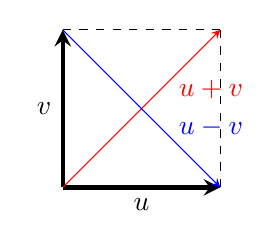
\begin{tikzpicture}
                \def\a{2}
                \pgfmathsetmacro{\b}{sqrt(2*\a*\a)};
                
                \draw[ultra thick, -stealth] (0,0) -- node[left] {$v$} (0,\a);
                \draw[ultra thick, -stealth] (0,0) -- node[below] {$u$} (\a,0);

                \draw[-stealth, red] (0,0) -- node[above right] {$\quad u+v$} (\a,\a);
                \draw[-stealth, blue] (0,\a) -- node[below right] {$\quad u-v$} (\a,0);

                \draw[dashed, thin] (0, \a) -- (\a,\a);
                \draw[dashed, thin] (\a, 0) -- (\a,\a);
            \end{tikzpicture}
        \end{figure}

        \item $\big| \;||u||-||v|| \;\big| \leq ||u-v||$.

        Como ambos términos son positivos, elevamos al cuadrado:
        \begin{equation*}\begin{split}
            \big| \;||u||-||v|| \;\big| &\leq ||u-v||
            \Longleftrightarrow \\ &\Longleftrightarrow (||u||-||v||)^2 \leq ||u-v||^2 
            \Longleftrightarrow \\ &\Longleftrightarrow
            ||u||^2 + ||v||^2 - 2||u||\;||v|| \leq ||u||^2 +||v||^2 -2g(u,v)
            \Longleftrightarrow \\ &\Longleftrightarrow
            - 2||u||\;||v|| \leq -2g(u,v)
            \Longleftrightarrow \\ &\Longleftrightarrow
             ||u||\;||v|| \geq g(u,v) \qquad \text{Cierto, por la desigualdad de Schwarz.}
        \end{split}\end{equation*}
    \end{enumerate}
\end{ejercicio}



\begin{ejercicio} Consideramos el EVME $(\bb{R}^3, \langle,\rangle)$, y sean $L_1,L_2\subset \bb{R}^3$ dos rectas vectoriales distintas. Sea $s_1=s_{L_1},s_2=s_{L_2}$. Demostrar que $f=s_1\circ s_2$ es un giro de eje $L$, siendo $L$ la única recta ortogonal a $L_1,L_2$. Calcular el ángulo del giro.\\

Sea $f=s_1\circ s_2$. Como la composición de isometrías es una isometría, tenemos que $f$ es una isometría.

Además, como $s_1,s_2$ son simetrías axiales, son simetrías directas. Por tanto, en cierta base se da que $|s_1| = |s_2| = 1$. Por tanto, $|f|=|s_1||s_2|=1\Longrightarrow f$ es una isometría directa, es decir, un giro sin simetría. Como $L_1\neq L_2\Longrightarrow f\neq Id$. Sea $L=\cc{L}\{e\}$ el eje de giro. Veamos que $L\perp L_1,L_2$.

Sea $U=L_1^\perp \cap L_2^\perp$, y consideramos $u\in U$:
\begin{equation*}
    f(u)=(s_1\circ s_2)(u) = s_1(-u) = u \Longrightarrow u\in V_1(f)=L
\end{equation*}

Por tanto, tengo que $U=L$, por lo que $L\perp L_1, L_2$. Calculemos ahora el ángulo.

Para ello, es necesario tomar un vector perpendicular al eje, por lo que consideramos $e_2$ tal que $L_2=\cc{L}\{e_2\}$ y $||e_2||=1$.
\begin{equation*}
    f(e_2) = s_1(s_2(e_2)) = s_1(e_2) = 2p_1(e_2) - e_2
\end{equation*}

Calculamos $p_1(e_2)$. Sea $e_1$ tal que $L_1=\cc{L}\{e_1\}$ y $||e_1||=1$. Sea $\cc{B}=\{e_1, w_1, w_2\}$ base ortonormal. Entonces:
\begin{equation*}
    p_1(e_2) = \left\langle e_1, e_2\right\rangle e_1
\end{equation*}

Denominemos $\alpha = \measuredangle \{e_1, e_2\} = \measuredangle \{L_1, L_2\}$. Entonces:
\begin{equation*}
    \cos \alpha = \frac{\langle e_1, e_2\rangle}{||e_1||\;||e_2||} = \langle e_1, e_2\rangle
\end{equation*}

Por tanto, tenemos que:
\begin{equation*}
    p_1(e_2) = \cos \alpha \cdot e_1 \Longrightarrow f(e_2) = 2\cos \alpha \cdot e_1 - e_2
\end{equation*}

Por tanto, definiendo $\theta$ como el ángulo de giro, tenemos que:
\begin{equation*}
    \cos \theta = \frac{\langle e_2, f(e_2)\rangle}{||e_2||^2} = \langle e_2, 2\cos \alpha \cdot e_1 - e_2\rangle = 2\cos \alpha \langle e_2, e_1\rangle - \langle e_2, e_2\rangle = 2\cos^2\alpha - 1
\end{equation*}

Por tanto, tenemos que $\theta = \arccos (2\cos^2 \alpha -1)$, siendo $\alpha$ el ángulo entre las dos rectas.

\end{ejercicio}


\begin{ejercicio} Consideramos $(\bb{R}^3, \langle,\rangle)$. Sean $v_1=\left(\begin{array}{c}
    1 \\ 1 \\ 0
\end{array}\right)$ y $v_2=\left(\begin{array}{c}
    1 \\ 0 \\ 1
\end{array}\right)$. Definimos los subespacios $L_1=\cc{L}\{v_1\}$, $L_2=\cc{L}\{v_2\}$. Calcular $f=s_2\circ s_1$.


    \begin{figure}[H]
	\centering
	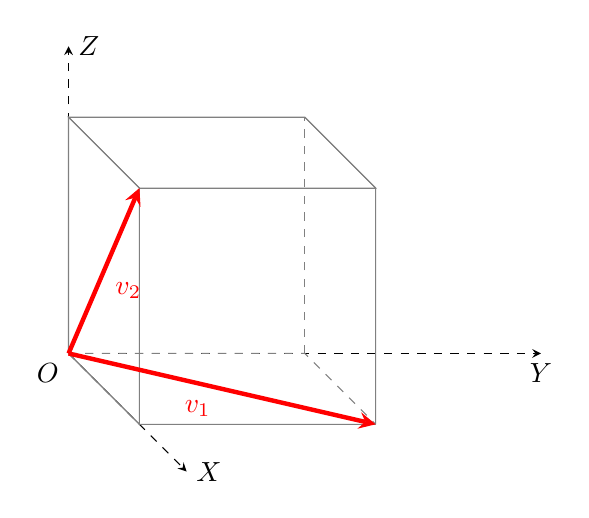
\begin{tikzpicture}[scale=3]
            
		% Definir las coordenadas de los vértices del cubo
		\coordinate (A) at (0,0);
		\coordinate (B) at (0,1);
		\coordinate (C) at (1,1);
		\coordinate (D) at (1,0);
		\coordinate (E) at (0.3,-0.3);
		\coordinate (F) at (0.3,0.7);
		\coordinate (G) at (1.3,0.7);
		\coordinate (H) at (1.3,-0.3);

  
            \draw[-stealth, dashed] (A) -- (2, 0); % Eje Y
            \node[below] at (2,0) {$Y$};
            \draw[-stealth, dashed] (A) -- (0, 1.3); % Eje Z
            \node[right] at (0,1.3) {$Z$};
            \draw[-stealth, dashed] (A) -- (0.5, -0.5); % Eje X
            \node[right] at (0.5,-0.5) {$X$};
		
		% Dibujar las caras del cubo
		%\draw[gray] (A) -- (B) -- (C) -- (D) -- cycle; % Cara trasera
            \draw[gray] (A) -- (B) -- (C); % Cara trasera
		\draw[gray] (H) -- (G) -- (C); % Cara frontal
		%\draw[gray] (A) -- (D) -- (H) -- (E) -- cycle; % Cara inferior
            \draw[gray] (A) -- (E) -- (H); % Cara inferior
		\draw[gray] (B) -- (C) -- (G) -- (F) -- cycle; % Cara superior
		\draw[gray] (A) -- (B) -- (F) -- (E) -- cycle; % Cara lateral izquierda
		%\draw[gray] (E) -- (F) -- (G) -- (H) -- cycle; % Cara lateral derecha
            \draw[gray] (E) -- (F) -- (G); % Cara lateral derecha
		
		% Dibujar las aristas ocultas
		\draw[gray, dashed] (A) -- (D) -- (H);
            \draw[gray, dashed] (D) -- (C);

            \draw[-stealth, red, ultra thick] (A) -- node[below right]{$v_2$} (F);
            \draw[-stealth, red, ultra thick] (A) -- node[below left]{$v_1$}(H);
		
		% Etiquetar el vértice de abajo a la izquierda como "O"
		\node[below left] at (A) {$O$};
        
        \end{tikzpicture}
    \end{figure}



    Por el ejercicio anterior, sabemos que es un giro de eje $L$ y ángulo $\theta$. Como el eje de giro es la única recta perpendicular a $L_1, L_2$, tenemos que $L=\cc{L}\{v_1\times v_2\}$, con:
    \begin{equation*}
        v_1\times v_2 = \left|\begin{array}{ccc}
            i & j & k \\
            1 & 1 & 0 \\
            1 & 0 & 1
        \end{array}\right| =  i-k-j = \left(\begin{array}{c}
            1 \\ -1 \\ -1
        \end{array}\right)
    \end{equation*}
    donde hemos hecho uso de que $\cc{B}_u = \{i,j,k\}$.

    Para calcular el ángulo, tomamos un vector perpendicular al eje. Sea el vector $v_1$ (también podría haber escogido $v_2$). Entonces:
    \begin{equation*}
        f(v_1)=(s_2\circ s_1)(v_1) = s_2(v_1) = 2p_2(v_1) - v_1
    \end{equation*}

    Calculamos por tanto $p_2(v_1)$. Tomamos como base $\cc{B}=\{\frac{v_2}{||v_2||}, w_1, w_2\}$ base ortonormal. Entonces:
    \begin{equation*}
        p_2(v_1)=\left\langle v_1,\frac{v_2}{||v_2||}\right\rangle  \cdot \frac{v_2}{||v_2||} = \langle v_1,v_2\rangle  \cdot \frac{v_2}{||v_2||^2} = 1\cdot \frac{v_2}{2} = \frac{1}{2}v_2
    \end{equation*}

    Por tanto,
    \begin{equation*}
        f(v_1)=2\cdot \frac{1}{2}v_2 - v_1 = v_2-v_1 = \left(\begin{array}{c}
            0 \\ -1 \\ 1
        \end{array}\right)
    \end{equation*}

    Por tanto, tenemos que:
    \begin{equation*}
        \cos \theta = \frac{\langle v_1, f(v_1)\rangle}{2} = -\frac{1}{2}
    \end{equation*}

    Por tanto, el ángulo no orientado es $\theta = \frac{2\pi}{3}$. De hecho, podemos observar que coincide con el resultado obtenido en el ejercicio anterior.
\end{ejercicio}


\begin{ejercicio}
    Sean $u,v,w\in V^2$, con $(V^2,g)$ EVME. Supongamos que:
    \begin{equation*}
        ||u||=||v||=||w||=1
        \qquad \land \qquad
        u+v+w=0
    \end{equation*}

    Demostrar que $\theta = \measuredangle \{u,v\}=\frac{2\pi}{3}$.\\


    Tenemos que $u+v=-w$. Tomando norma, tenemos que:
    \begin{equation*}
        ||w||^2=1 = ||u+v||^2 = ||u||^2 + ||v||^2 + 2g(u,v) \Longrightarrow 1=2+2g(u,v) \Longrightarrow g(u,v)=-\frac{1}{2}
    \end{equation*}

    Por la definición del coseno entre dos ángulos, tenemos que:
    \begin{equation*}
        \cos \theta = \frac{g(u,v)}{||u||\;||v||} = \frac{-\frac{1}{2}}{1} = -\frac{1}{2} \Longrightarrow \theta = \frac{2\pi}{3}
    \end{equation*}

    Por tanto, queda demostrado que $\theta = \measuredangle \{u,v\}=\frac{2\pi}{3}$.
\end{ejercicio}


\begin{ejercicio}\label{Ej42.SimRectaAng}
    Sea el EVME $(\bb{R}^2,\;\langle,\rangle)$, y consideramos la recta $L=\cc{L}\{e\}$ tal que el ángulo que forma la recta con el eje $OX$ es $\theta$.

    \begin{figure}[H]
        \centering
        \begin{tikzpicture}
            \def\x{2}
            \def\y{1}
            \draw[-stealth] (-0.5, 0) -- (3, 0) node[right] {Eje $X$};
            \draw[-stealth] (0, -0.5) -- (0, 3) node[above] {Eje $Y$};
            
            \draw[thick, -stealth] (0, 0) -- (\x, \y) node[above] {$e$};
            \draw[] (-0.5*\x, -0.5*\y) -- (2*\x, 2*\y) node[above right] {${L}$};
            \draw (0.5, 0) arc (0:25:0.5) node[midway, right] {$\theta$};
        \end{tikzpicture}
    \end{figure}

    Sea $e=\left(\begin{array}{c}
        a \\ b
    \end{array}\right)$ vector unitario. Demostrar que:
    \begin{equation*}
        M(s_L;\cc{B}_u) = \left(\begin{array}{cc}
            a^2-b^2 & 2ab \\
            2ab & -a^2+b^2
        \end{array}\right)
    \end{equation*}

    Tenemos que $L=\cc{L}\left\{\left(\begin{array}{c}
        a \\ b
    \end{array}\right)\right\}$, por lo que $L^\perp=\cc{L}\left\{\left(\begin{array}{c}
        -b \\ a
    \end{array}\right)\right\}$

    Por tanto, y teniendo en cuenta que $||e||=1$, tenemos que una base ortonormal de $\bb{R}^2$ es:
    \begin{equation*}
        \cc{B}=\{e_1, e_2\} = \left\{
        \left(\begin{array}{c}
            a \\ b
        \end{array}\right),
        \left(\begin{array}{c}
            -b \\ a
        \end{array}\right)
        \right\}
    \end{equation*}

    Para obtener la matriz asociada a la base usual, sea $v\in \bb{R}^2$, con coordenadas
    \begin{equation*}
        v=\left(\begin{array}{c}
                 x_1 \\ x_2
            \end{array}\right)_{\cc{B}_u}
            =\left(\begin{array}{c}
                 a_1 \\ a_2
            \end{array}\right)_{\cc{B}}
    \end{equation*}

    Por ser $\cc{B}$ una base ortonormal, tenemos que:
    \begin{equation*}
        a_1 = \left\langle 
            v, e_1\right\rangle
            = \left\langle 
            \left(\begin{array}{c}
                 x_1 \\ x_2
            \end{array}\right),
            \left(\begin{array}{c}
                 a \\ b
            \end{array}\right)
            \right\rangle
            = (ax_1+bx_2)
    \end{equation*}
    \begin{equation*}
        a_2 = \left\langle 
            v, e_2\right\rangle
            = \left\langle 
            \left(\begin{array}{c}
                 x_1 \\ x_2
            \end{array}\right),
            \left(\begin{array}{c}
                 -b \\ a
            \end{array}\right)
            \right\rangle
            = (-bx_1+ax_2)
    \end{equation*}

    Por tanto, tenemos que:
    \begin{equation*}
        \begin{split}
            s_L(v)& = s_L(a_1e_1+a_2e_2) = a_1e_1-a_2e_2 =\\
            &= (ax_1+bx_2)\left(\begin{array}{c}
                 a \\ b
            \end{array}\right) -(-bx_1+ax_2)\left(\begin{array}{c}
                 -b \\ a
            \end{array}\right) =\\
            &= \left(\begin{array}{c}
                 a^2x_1 +abx_2 \\ abx_1+b^2x_2
            \end{array}\right)
            + \left(\begin{array}{c}
                 -b^2x_1 +abx_2 \\ abx_1-a^2x_2
            \end{array}\right) =\\
            &= \left(\begin{array}{c}
                 (a^2-b^2)x_1+2abx_2 \\ 2abx_1 + (b^2-a^2)x_2
            \end{array}\right)
            = \left(\begin{array}{cc}
                 a^2-b^2 & 2ab \\
                 2ab & -a^2 + b^2
            \end{array}\right)
            \left(\begin{array}{c}
                 x_1 \\ x_2
            \end{array}\right)
        \end{split}
    \end{equation*}

    Por tanto, como queríamos demostrar, tenemos que
    \begin{equation*}
        M(s_L;\cc{B}_u) = \left(\begin{array}{cc}
            a^2-b^2 & 2ab \\
            2ab & -a^2+b^2
        \end{array}\right)
    \end{equation*}


    Por tanto, como $||e||=1$ es unitario, tenemos que $a^2+b^2=1$. Suponiendo que $\theta \in [0,\pi/2]$, tenemos que:
    \begin{equation*}
        e=\left(\begin{array}{c}
            a \\ b
        \end{array}\right)
        = \left(\begin{array}{c}
            \cos \theta \\ \sen \theta
        \end{array}\right)
    \end{equation*}

    Por tanto, la matriz respecto de la base usual en función del ángulo es:
    \begin{equation*}
        M(s_L;\cc{B}_u) = \left(\begin{array}{cc}
            \cos^2 \theta - \sen^2\theta & 2\cos\theta\sen \theta \\
            2\cos\theta\sen \theta & -\cos^2 \theta+ \sen ^2 \theta
        \end{array}\right)
        = \left(\begin{array}{cc}
            \cos(2\theta) & \sen(2\theta) \\
            \sen(2\theta) & -\cos(2\theta)
        \end{array}\right)
    \end{equation*}

    
        
\end{ejercicio}



\begin{ejercicio}
    Sea $f\in Iso(V^n, g)$. Demostrar que $h=f+f^{-1}$ es un endomorfismo autoadjunto.\\

    Tenemos que comprobar que se tiene lo siguiente:
    \begin{equation*}
        g(h(u), v) = g(u, h(v)) \hspace{2cm} \forall u,v\in V
    \end{equation*}

    Como $g$ es una forma bilineal, tenemos que:
    \begin{equation*}
        g(h(u), v) = g[f(u)+f^{-1}(u), v]
        = g[f(u), v] + g[f^{-1}(u), v]
    \end{equation*}

    Como $f$ es una isometría, $f^{-1}$ también lo es, ya que la inversa de una matriz ortogonal también es ortogonal. Por tanto, $f^{-1}$ conserva las métricas. Aplicando $f^{-1}$ a la primera métrica y $f$ a la segunda, tenemos que:
    \begin{multline*}
        g(h(u), v) = g[f^{-1}(f(u)), f^{-1}(v)] + g[f(f^{-1}(u)), f(v)]
        =\\= g(u, f^{-1}(v)) + g(u, f(v))
        = g(u, f(v) + f^{-1}(v))
        = g(u, h(v))
    \end{multline*}

    Como esto se cumple $\forall v\in V$, tenemos que $h$ es un endomorfismo autoadjunto.
    
\end{ejercicio}


\begin{ejercicio}
    Sea el EVME $(\bb{R}^2, g)$ con:
    \begin{equation*}
        G=M(g;\cc{B}_u) = \left(\begin{array}{cc}
            3 & 3 \\
            3 & 4
        \end{array}\right)
    \end{equation*}

    Encontrar la matriz respecto de $\cc{B}_u$ de un giro de ángulo $\theta = \frac{\pi}{2}$.\\

    Tenemos que:
    \begin{equation*}
        \cos \theta = 0 = \frac{g(u,f(u))}{||u||^2} \Longrightarrow g(u,f(u)) = 0 \quad \forall u\in V
    \end{equation*}

    Sea $\cc{B}_u = \{e_1, e_2\}$. Consideramos $f(e_1)=\left(\begin{array}{c}
            a \\ b
        \end{array}\right)$. Entonces:
    \begin{equation*}
        g(e_1, f(e_1)) = 0 = e_1 \left(\begin{array}{cc}
            3 & 3 \\
            3 & 4
        \end{array}\right) \left(\begin{array}{c}
            a \\ b
        \end{array}\right) = \left(\begin{array}{cc}
            3 & 3 \\
        \end{array}\right) \left(\begin{array}{c}
            a \\ b
        \end{array}\right)
        = 3a + 3b \Longrightarrow a=-b
    \end{equation*}
    Por tanto, sea $f(e_1)=\left(\begin{array}{c}
            -\alpha \\ \alpha
        \end{array}\right)$. Además, al ser $f$ una isometría, tenemos que conserva las métricas. Por tanto,
    \begin{multline*}
        ||e_1|| = ||f(e_1)|| \Longrightarrow ||e_1||^2 = ||f(e_1)||^2 \Longrightarrow
        1 = g(f(e_1), f(e_1)) = \\
        = \left(\begin{array}{cc}
            -\alpha & \alpha
        \end{array}\right)
        \left(\begin{array}{cc}
            3 & 3 \\
            3 & 4
        \end{array}\right) \left(\begin{array}{c}
            -\alpha \\ \alpha
        \end{array}\right)
        = \left(\begin{array}{cc}
            0 & \alpha
        \end{array}\right)
        \left(\begin{array}{c}
            -\alpha \\ \alpha
        \end{array}\right) = \alpha^2 \Longrightarrow \alpha = \pm 1
    \end{multline*}
    Por tanto, sea $$f(e_1)=\left(\begin{array}{c}
            -\alpha \\ \alpha
        \end{array}\right) \qquad \alpha = \pm 1$$

    Consideramos ahora $f(e_2)=\left(\begin{array}{c}
            c \\ d
        \end{array}\right)$. Entonces:
    \begin{equation*}
        g(e_2, f(e_2)) = 0 = e_2 \left(\begin{array}{cc}
            3 & 3 \\
            3 & 4
        \end{array}\right) \left(\begin{array}{c}
            c \\ d
        \end{array}\right) = \left(\begin{array}{cc}
            3 & 4 \\
        \end{array}\right) \left(\begin{array}{c}
            c \\ d
        \end{array}\right)
        = 3c + 4d \Longrightarrow 3c=-4d
    \end{equation*}
    Por tanto, sea $f(e_2)=\left(\begin{array}{c}
            -4\beta \\ 3\beta
        \end{array}\right)$. Además, al ser $f$ una isometría, tenemos que conserva las métricas. Por tanto,
    \begin{multline*}
        ||e_2|| = ||f(e_2)|| \Longrightarrow ||e_2||^2 = ||f(e_2)||^2 \Longrightarrow
        1 = g(f(e_2), f(e_2)) = \\
        = \left(\begin{array}{cc}
            -4\beta & 3\beta
        \end{array}\right)
        \left(\begin{array}{cc}
            3 & 3 \\
            3 & 4
        \end{array}\right) \left(\begin{array}{c}
            -4\beta \\ 3\beta
        \end{array}\right)
        = \left(\begin{array}{cc}
            -3\beta & 0
        \end{array}\right)
        \left(\begin{array}{c}
            -4\beta \\ 3\beta
        \end{array}\right) = 12\beta^2 \Longrightarrow \beta = \pm \frac{1}{\sqrt{12}}
    \end{multline*}
    Por tanto, sea $$f(e_2)=\left(\begin{array}{c}
            -4\beta \\ 3\beta
        \end{array}\right) \qquad \beta = \pm \frac{1}{\sqrt{12}}$$


    Por tanto, sea la matriz del giro de $\theta = \frac{\pi}{2}$ la siguiente:
    \begin{equation*}
        M(G_\theta;\cc{B}_u) = \left(\begin{array}{cc}
            -\alpha & -4\beta \\
            \alpha & 3\beta
        \end{array}\right) \qquad \beta = \frac{1}{\sqrt{12}} \qquad \alpha = \pm 1
    \end{equation*}

    La existencia de los dos valores de $\alpha$ se debe a que el ángulo dado es no orientado, por lo que hay dos posibles soluciones.
\end{ejercicio}



\begin{ejercicio}
    Consideramos el espacio vectorial $\bb{R}_2[x]$, y consideramos su base $\cc{B}=~\{1,x,x^2\}$.
    \begin{enumerate}
        \item Demostrar que la métrica definida por
        \begin{equation*}
            g(p,q) = \int_0^1 p(x)q(x)\;dx
        \end{equation*}
        es, efectivamente, una métrica.

        Tenemos que, claramente, es bilineal. Además,
        \begin{equation*}
            g(p,p)=\int_0^1 p^2(x)\,dx
        \end{equation*}
        como el integrando es positivo, tenemos que $g(p,p)>0\qquad \forall p\in \bb{R}_2[x]-\{0\}$. Por tanto, tenemos que es una métrica.


        \item Aplicar Gram-Schmidt con la métrica $g$ para hallar una base ortogonal.

        Sea $\cc{B}_o = \{e_1, e_2, e_3\}$ y partimos desde $e_1 = 1$. Entonces:
        \begin{equation*}
            e_2 = x - \frac{g(1,x)}{g(1,1)} = x-\frac{1}{2}
        \end{equation*}

        Además, tenemos que:
        \begin{equation*}
            e_3 = x^2 - \frac{g(1,x^2)}{g(1,1)} - \frac{g\left(x-\frac{1}{2},x^2\right)}{g\left( x-\frac{1}{2}, x-\frac{1}{2}\right)}\left(x-\frac{1}{2}\right) = x^2-\frac{1}{3} - x-\frac{1}{2} = x^2 -x -\frac{5}{6}
        \end{equation*}

        Por tanto, tenemos que la base ortogonal es:
        \begin{equation*}
            \cc{B}_o = \left\{1, x-\frac{1}{2}, x^2-x-\frac{5}{6}\right\}
        \end{equation*}
    \end{enumerate}
\end{ejercicio}


\begin{ejercicio}
    Sea la forma cuadrática $F\in End(\bb{R}^3)$ tal que, en la base usual,
    \begin{equation*}
        F(x,y,z) = 2\left(x^2-z^2+xy+yz\right)
    \end{equation*}

    Estudiar la figura $\xi \equiv F(x,y,z)=0$.\\

    En primer lugar, tenemos que la matriz de la métrica asociada a dicha forma cuadrática es:
    \begin{equation*}
        A = M(g,\cc{B}_u) = \left(\begin{array}{ccc}
            2 & 1 & 0\\
            1 & 0 & 1 \\
            0 & 1 & -2
        \end{array}\right)
    \end{equation*}

    En primer lugar, obtenemos la matriz asociada a la base de Sylvester. Para ello, tenemos que $|A|=0$, por lo que $rg(A)=2$. Además, tenemos que es indefinida, por lo que:
    \begin{equation*}
        A_s = M(g,\cc{B}_s) = \left(\begin{array}{ccc}
            1 &\\
             & -1 & \\
             &  & 0
        \end{array}\right)
    \end{equation*}

    Por tanto, en la base de Sylvester tenemos que:
    \begin{equation*}
        F(\bar{x}, \bar{y}, \bar{z}) = \bar{x}^2 - \bar{y}^2 = 0 \Longleftrightarrow \bar{x}^2 = \bar{y}^2 \Longrightarrow \bar{x}=\pm \bar{y}
    \end{equation*}

    Por tanto, tenemos que se trata de dos planos.
    
    
    Para calcular qué planos son, calculamos la base de Sylvester. Sea $\cc{B}=\{\bar{e_1},\bar{e_2},\bar{e_3}\}$.
    
    Definimos $\bar{e_1} = \frac{1}{\sqrt{2}}e_1$, y $\bar{e_2} = \frac{1}{\sqrt{2}}e_3$. Por último, escogemos $\bar{e_3}\in Ker(g)$.
    \begin{equation*}
        \bar{e_3} = v\in \bb{R}^3 \left|\left\{ \begin{array}{l}
            2x+y=0  \\
            x+z=0 \\
            y-2z=0
        \end{array}\right.\right.
    \end{equation*}

    Por tanto, sea la base de Sylvester:
    \begin{equation*}
        \cc{B}_s = \left\{\frac{1}{\sqrt{2}}\left(\begin{array}{c}
            1 \\ 0 \\ 0
        \end{array}\right),
        \frac{1}{\sqrt{2}}\left(\begin{array}{c}
            0 \\ 0 \\ 1
        \end{array}\right),
        \frac{1}{\sqrt{2}}\left(\begin{array}{c}
            -1 \\ 2 \\ 1
        \end{array}\right)\right\}
    \end{equation*}

    Por tanto, tenemos que:
    \begin{equation*}
        P=M(\cc{B}_s;\cc{B}_u) = \frac{1}{\sqrt{2}}\left(\begin{array}{ccc}
            1 & 0 & -1 \\
            0 & 0 & 2 \\
            0 & 1 & 1 \\
        \end{array}\right)
    \end{equation*}

    Por tanto, usando que esa matriz es la matriz de cambio de base, tenemos que:
    \begin{equation*}
        \left(\begin{array}{ccc}
            {x} \\ {y} \\ {z}
        \end{array}\right) = \frac{1}{\sqrt{2}}\left(\begin{array}{ccc}
            1 & 0 & -1 \\
            0 & 0 & 2 \\
            0 & 1 & 1 \\
        \end{array}\right)
        \left(\begin{array}{ccc}
            \bar{x} \\ \bar{y} \\ \bar{z}
        \end{array}\right)
        \Longrightarrow
        \left(\begin{array}{ccc}
            {x} \\ {y} \\ {z}
        \end{array}\right) = \frac{1}{\sqrt{2}}\left(\begin{array}{c}
            \bar{x}-\bar{z}\\ 2\bar{z}\\\bar{y}+\bar{z}
        \end{array}\right)
    \end{equation*}

    Igualando cada componente, tenemos que:
    \begin{equation*}
        \left\{\begin{array}{l}
            \bar{z} = \frac{\sqrt{2}}{2}y \\
            \bar{y} = \sqrt{2}z - \bar{z} = \sqrt{2}z - \frac{\sqrt{2}}{2}y \\
            \bar{x} = \sqrt{2}x + \bar{z} = \sqrt{2}x + \frac{\sqrt{2}}{2}y \\
        \end{array}\right.
    \end{equation*}

    Por tanto, como la ecuación de la figura estudiada es $\xi \equiv \bar{x}=\pm \bar{y}$, tenemos que:
    \begin{equation*}
        \xi \equiv \sqrt{2}x + \frac{\sqrt{2}}{2}y = \pm \left(\sqrt{2}z - \frac{\sqrt{2}}{2}y\right)
    \end{equation*}

    Los dos planos son los que tienen por ecuación:
    \begin{equation*}
        \Pi_1 \equiv \sqrt{2}x +\sqrt{2}z=0 \equiv x-z=0
        \qquad
        \Pi_1 \equiv \sqrt{2}x -\sqrt{2}z + \sqrt{2}y=0 \equiv x+y-z=0
    \end{equation*}
\end{ejercicio}



\begin{ejercicio}
    Dado $A\in \cc{S}_n(\bb{R})$, demostrar que:
    \begin{equation*}
        tr^2(A) \leq n\;tr(A^2) \qquad \forall A\in \cc{S}_n(\bb{R})
    \end{equation*}

    En primer lugar, definimos la siguiente aplicación bilineal en $\cc{S}_n(\bb{R})$:
    \begin{equation*}
        g(A,B) = tr(AB)
    \end{equation*}

    Veamos que se trata de una métrica definida positiva. Calculamos en primer lugar $A^2$:
    \begin{equation*}
        A^2 = (c_{ij})_{i,j} \qquad c_{ij}=\sum_{k=1}^n a_{ik}a_{kj}
    \end{equation*}
    
    Por tanto,
    \begin{equation*}
        g(A,A) = tr(A^2) = \sum_{i=1}^n c_{ii} = \sum_{i,k=1}^n a_{ik}a_{ki}
        = \sum_{i,k=1}^n a_{ik}^2
        \geq 0
    \end{equation*}

    donde he empleado que, por ser $A$ simétrica, $a_{ij}=a{ji}$. Además, tenemos que: $$g(A,A)=0 \Longleftrightarrow a_{ik}=0 \quad \forall i,k=1,\dots, n\Longleftrightarrow A=0$$

    Por tanto, tenemos que $(\cc{S}_n(\bb{R}), g)$ es un EVME. Por tanto, se cumple la desigualdad de Schwarz. Entonces, amplicando dicha desigualdad a $A,I_n$ tenemos que:
    \begin{equation*}
        g^2(A,I) \leq ||A||^2 ||I||^2\Longrightarrow tr^2(AI) \leq tr(A^2)\;tr(I_n^2) \Longrightarrow tr^2(A)\leq n\;tr(A^2)
    \end{equation*}

    Además, tenemos que la igualdad se da solo si $A=aI,\;a\in \bb{R}$.
\end{ejercicio}


\begin{ejercicio}
    Sea $(\bb{R}^3, \langle,\rangle)$ el espacio vectorial euclídeo dado por el producto escalar y $U_1,U_2\subset \bb{R}^3$ dos planos vectoriales distintos.
    \begin{enumerate}
        \item Demostrar que existe una simetría axial $s\in End(\bb{R}^3)$ verificando:
        \begin{equation*}
            s(U_1)=U_1 \hspace{2cm} s(U_2)=U_2
        \end{equation*}

        Consideramos el subespacio vectorial $L=U_1\cap U_2$. Como los planos son distintos, se cortan en una recta. Sea la recta $L=\cc{L}\{e\}$. Como $L=U_1\cap U_2$, tenemos que:
        \begin{gather*}
            L\subset U_1 \Longrightarrow U_1=\cc{L}\{e, e_1\} \\
            L\subset U_2 \Longrightarrow U_2=\cc{L}\{e, e_2\}
        \end{gather*}

        Suponemos sin pérdida de generalidad que $e_1,e_2\perp e$, por lo que $e_1,e_2\in L^\perp$. Por tanto,
        \begin{gather*}
            \forall u_1=ae+be_1\in U_1,\quad s(u_1)=ae-be_1\in U_1 \Longrightarrow s(U_1)\subset U_1 \\
            \forall u_2=ae+be_2\in U_2,\quad s(u_2)=ae-be_2\in U_2 \Longrightarrow s(U_2)\subset U_2
        \end{gather*}

        Por tanto, la simetría respecto de $L$ cumple lo pedido.


        \item Si consideramos los planos vectoriales
        \begin{equation*}
            U_1 = \{(x, y, z) \in \bb{R}^3 \mid x + y = 0\}
            \qquad
            U_2 = \{(x, y, z) \in \bb{R}^3 \mid x - z = 0\}
        \end{equation*}

        encontrar la matriz de $s$ respecto de la base usual.

        Sea $\cc{B}_u=\{e_1, e_2, e_3\}$. Tenemos que, en este caso, $U=\cc{L}\left\{\left(\begin{array}{c}
            1 \\ -1 \\ 1
        \end{array}\right)\right\} = \{e_1-e_2+e_3\}$. Por tanto, tenemos que:
        \begin{equation*}
            U^\perp = \cc{L}\left\{
            \left(\begin{array}{c}
                1 \\ 1 \\ 0
            \end{array}\right),
            \left(\begin{array}{c}
                1 \\ 0 \\ -1
            \end{array}\right)
            \right\} = \{e_1+e_2, e_1-e_3\}
        \end{equation*}

        Por tanto, sabiendo que $U=V_1, U^\perp = V_{-1}$, tenemos que:
        \begin{equation*}
            \left\{\begin{array}{rl}
                s_U(e_1-e_2+e_3) &= e_1-e_2+e_3 = s_U(e_1) -s_U(e_2) + s_U(e_3) \\
                s_U(e_1+e_2) &= -e_1-e_2 = s_U(e_1) +s_U(e_2) \Longrightarrow s_U(e_2) = -s_U(e_1)-e_1-e_2\\
                s_U(e_1-e_3) &= -e_1+e_3 = s_U(e_1) -s_U(e_3) \Longrightarrow s_U(e_3)=s_U(e_1)+e_1-e_3\\
            \end{array}\right.
        \end{equation*}
        Sustituyendo en la primera ecuación, tenemos:
        \begin{equation*}
            e_1-e_2+e_3 = s_U(e_1) +s_U(e_1)+e_1+e_2 + s_U(e_1)+e_1-e_3
        \end{equation*}

        Por tanto, tenemos:
        \begin{equation*}
            \left\{\begin{array}{l}
                3s_U(e_1) = -e_1-2e_2+2e_3 \\
                3s_U(e_2) = -3s_U(e_1)-3e_1-3e_2 = e_1+2e_2-2e_3 -3e_1-3e_2 = -2e_1-e_2-2e_3\\
                3s_U(e_3) = 3s_U(e_1)+3e_1-3e_3 = -e_1-2e_2+2e_3+3e_1-3e_3 = 2e_1-2e_2-e_3
            \end{array}\right.
        \end{equation*}

        Por tanto, la matriz buscada es:
        \begin{equation*}
            M(s_U, \cc{B}_u) = \frac{1}{3}\left(\begin{array}{ccc}
                -1 & -2 & 2 \\
                -2 & -1 & -2\\
                2 & -2 & -1
            \end{array}\right)
        \end{equation*}
    \end{enumerate}
\end{ejercicio}



\begin{ejercicio}
    Para cada $a\in \bb{R}$ consideramos la forma cuadrática $F_a:\bb{R}^3\to \bb{R}$
    \begin{equation*}
        F_a(x_1, x_2, x_3) = ax_1^2 + x_2^2 + 2(1 - a)x_1x_3 + ax_3^2
    \end{equation*}

    Sea $g_a$ su métrica asociada:
    \begin{enumerate}
        \item Calcular el núcleo de $g_a$.

        En primer lugar, calculamos la matriz asociada a $g_a$:
        \begin{equation*}
            G_a = M(g_a, \cc{B}_u) = \left(\begin{array}{ccc}
                a & 0 & 1-a \\
                0 & 1 & 0 \\
                1-a & 0 & a
            \end{array}\right)
        \end{equation*}

        Calculamos el determinante para calcular el rango:
        \begin{equation*}
            |G_a| = a^2 -(1-a)^2 = a^2 -a^2 -1 +2a = 2a-1 = 0\Longleftrightarrow a=\frac{1}{2}
        \end{equation*}

        Por tanto,
        \begin{itemize}
            \item \underline{Para $a\neq \frac{1}{2}$}:

            Tenemos que $g_a$ es no degenerada, por lo que $Ker(g_a)=\{0\}$.

            \item \underline{Para $a = \frac{1}{2}$}:

            Tenemos que $rg(G_a)=2$, por lo que $\dim Ker(g_a) = 1$.
            \begin{equation*}
                \begin{split}
                    Ker(g_a) &= \left\{\left(\begin{array}{c}
                        x \\ y \\ z
                    \end{array}\right)\in \bb{R}^3 \left|
                    \left(\begin{array}{ccc}
                        \frac{1}{2} & 0 & \frac{1}{2} \\
                        0 & 1 & 0 \\
                        \frac{1}{2} & 0 & \frac{1}{2}
                    \end{array}\right)
                    \left(\begin{array}{c}
                        x \\ y \\ z
                    \end{array}\right) = 0
                    \right.\right\} \\
                    &= \cc{L}\left\{\left(\begin{array}{c}
                        1 \\ 0 \\ -1
                    \end{array}\right)\right\}
                \end{split}
            \end{equation*}
        \end{itemize}

        \item Clasificar la métrica en función del parámetro $a$:
        \begin{itemize}
            \item \underline{Para $a=\frac{1}{2}$}: Tenemos que $Nul(g_a)=1$. Además, para $U=\cc{L}\{e_2, e_3\}$, tenemos que la restricción es definida positiva. Por tanto, tenemos que:
            \begin{equation*}
                Nul(g_a)=1 \qquad Ind(g_a)=0
            \end{equation*}
            En este caso $g_a$ es semidefinida positiva.

            \item \underline{Para $a>\frac{1}{2}$}: Tenemos que $|G_a|>0$. Además, tenemos $G_a$ es definida positiva al ser todos sus menores principales positivos, por lo que $g_a$ también es definida positiva.

            \item \underline{Para $a <\frac{1}{2}$}: Tenemos que $|G_a|<0$. Además, $g_a(e_2, e_2)=1>0$, tenemos que $g_a$ tiene al menos un 1 en la matriz asociada a la base de Sylvester. Por tanto, como $Nul(g_a)=0$ y $|G_a|<0$, es necesario que:
            \begin{equation*}
                G_a\sim_c \left(\begin{array}{ccc}
                    1 &  \\
                     & 1 &  \\
                    &  & -1
                \end{array}\right)
            \end{equation*}

            Por tanto, $g_a$ es indefinida y $Nul(g_a)=0$, $Ind(g_a)=1$.
        \end{itemize}

        \item Resolver $F_a(x_1, x_2, x_3) = 0$ para $a = 3$ y $a = \frac{1}{2}$.


        Tenemos que:
        \begin{equation*}
            F_a\left(\begin{array}{c}
                        x \\ y \\ z
                    \end{array}\right)
            =\left(\begin{array}{cccc}
                        x & y & z
                    \end{array}\right) 
            G_a
            \left(\begin{array}{c}
                        x \\ y \\ z
                    \end{array}\right) = 0
        \end{equation*}

        Por tanto,
        \begin{equation*}
            F_a\left(\begin{array}{c}
                        x \\ y \\ z
                    \end{array}\right)
            = 0 \equiv \left\{v\in \bb{R}^3 \mid g_a(v,v)=0\right\}
        \end{equation*}

        \begin{itemize}
            \item \underline{Para $a=3$}:

            Tenemos que $g_a$ es definida positiva. Por tanto, el único vector con cuadrado nulo es $v=0$. Por tanto, la solución es un punto, el origen.

            \item \underline{Para $a=\frac{1}{2}$}:

            Tenemos que $g_a$ es semidefinida positiva. Por tanto, los vectores con cuadrado $0$ son los del núcleo. En apartados anteriores hemos demostrado que, en este caso,
            \begin{equation*}
                    Ker(g_a) = \cc{L}\left\{\left(\begin{array}{c}
                        1 \\ 0 \\ -1
                    \end{array}\right)\right\}
            \end{equation*}

            Por tanto, la solución es esa recta.
        \end{itemize}
        
    \end{enumerate}
\end{ejercicio}

